% **************************************************************************************************************
% A Classic Thesis Style
% An Homage to The Elements of Typographic Style
%
% Copyright (C) 2012 Andr\'e Miede http://www.miede.de
%
% If you like the style then I would appreciate a postcard. My address 
% can be found in the file ClassicThesis.pdf. A collection of the 
% postcards I received so far is available online at 
% http://postcards.miede.de
%
% License:
% This program is free software; you can redistribute it and/or modify
% it under the terms of the GNU General Public License as published by
% the Free Software Foundation; either version 2 of the License, or
% (at your option) any later version.
%
% This program is distributed in the hope that it will be useful,
% but WITHOUT ANY WARRANTY; without even the implied warranty of
% MERCHANTABILITY or FITNESS FOR A PARTICULAR PURPOSE.  See the
% GNU General Public License for more details.
%
% You should have received a copy of the GNU General Public License
% along with this program; see the file COPYING.  If not, write to
% the Free Software Foundation, Inc., 59 Temple Place - Suite 330,
% Boston, MA 02111-1307, USA.
%
% **************************************************************************************************************
% Note:
%    * You must not use "u etc. in strings/commands that will be spaced out (use \"u or real umlauts instead)
%    * New enumeration (small caps): \begin{aenumerate} \end{aenumerate}
%    * For margin notes: \marginpar or \graffito{}
%    * Do not use bold fonts in this style, it is designed around them
%    * Use tables as in the examples
%    * See classicthesis-preamble.sty for useful commands
% **************************************************************************************************************
% To Do:
%		 * [high] Check this out: http://www.golatex.de/koma-script-warnung-in-verbindung-mit-listings-package-t2058.html
%    * [medium] mathbb in section-titles/chapter-titles => disappears somehow in headlines!!!
% **************************************************************************************************************
\documentclass[ twoside,openright,titlepage,numbers=noenddot,headinclude,%1headlines,% letterpaper a4paper
                footinclude=true,cleardoublepage=empty,abstractoff, % <--- obsolete, remove (todo)
                BCOR=5mm,paper=a4,fontsize=11pt,%11pt,a4paper,%
                ngerman,american,%
                ]{scrreprt}

%********************************************************************
% Note: Make all your adjustments in here
%*******************************************************
% ****************************************************************************************************
% classicthesis-config.tex 
% formerly known as loadpackages.sty, classicthesis-ldpkg.sty, and classicthesis-preamble.sty 
% Use it at the beginning of your ClassicThesis.tex, or as a LaTeX Preamble 
% in your ClassicThesis.{tex,lyx} with % ****************************************************************************************************
% classicthesis-config.tex 
% formerly known as loadpackages.sty, classicthesis-ldpkg.sty, and classicthesis-preamble.sty 
% Use it at the beginning of your ClassicThesis.tex, or as a LaTeX Preamble 
% in your ClassicThesis.{tex,lyx} with % ****************************************************************************************************
% classicthesis-config.tex 
% formerly known as loadpackages.sty, classicthesis-ldpkg.sty, and classicthesis-preamble.sty 
% Use it at the beginning of your ClassicThesis.tex, or as a LaTeX Preamble 
% in your ClassicThesis.{tex,lyx} with \input{classicthesis-config}
% ****************************************************************************************************  
% If you like the classicthesis, then I would appreciate a postcard. 
% My address can be found in the file ClassicThesis.pdf. A collection 
% of the postcards I received so far is available online at 
% http://postcards.miede.de
% ****************************************************************************************************

% ****************************************************************************************************
% 1. Configure classicthesis for your needs here, e.g., remove "drafting" below 
% in order to deactivate the time-stamp on the pages
% ****************************************************************************************************
\PassOptionsToPackage{eulerchapternumbers,listings,drafting,%
				 pdfspacing,%floatperchapter,%linedheaders,%
				 subfig,beramono,eulermath,parts}{classicthesis}										
% ********************************************************************
% Available options for classicthesis.sty 
% (see ClassicThesis.pdf for more information):
% drafting
% parts nochapters linedheaders
% eulerchapternumbers beramono eulermath pdfspacing minionprospacing
% tocaligned dottedtoc manychapters
% listings floatperchapter subfig
% ********************************************************************

% ********************************************************************
% Triggers for this config
% ******************************************************************** 
\usepackage{ifthen}
\newboolean{enable-backrefs} % enable backrefs in the bibliography
\setboolean{enable-backrefs}{true} % true false
% ****************************************************************************************************


% ****************************************************************************************************
% 2. Personal data and user ad-hoc commands
% ****************************************************************************************************
\newcommand{\myTitle}{Patterns in Riordan arrays\xspace}
\newcommand{\mySubtitle}{characterizations respect to modular arithmetic and to function $h$\xspace}
\newcommand{\myDegree}{Doctor\xspace}
\newcommand{\myName}{Massimo Nocentini\xspace}
\newcommand{\myProf}{Donatella Merlini\xspace}
\newcommand{\myOtherProf}{Put name here\xspace}
\newcommand{\mySupervisor}{Put name here\xspace}
\newcommand{\myFaculty}{{S}cienze {M}atematiche {F}isiche e {N}aturali\xspace}
\newcommand{\myDepartment}{Put data here\xspace}
\newcommand{\myUni}{Universit\`a di Firenze\xspace}
\newcommand{\myLocation}{Firenze\xspace}
\newcommand{\myTime}{July 2015\xspace}
\newcommand{\myVersion}{version 0.1\xspace}

% ********************************************************************
% Setup, finetuning, and useful commands
% ********************************************************************
\newcounter{dummy} % necessary for correct hyperlinks (to index, bib, etc.)
\newlength{\abcd} % for ab..z string length calculation
\providecommand{\mLyX}{L\kern-.1667em\lower.25em\hbox{Y}\kern-.125emX\@}
\newcommand{\ie}{i.\,e.}
\newcommand{\Ie}{I.\,e.}
\newcommand{\eg}{e.\,g.}
\newcommand{\Eg}{E.\,g.} 
% ****************************************************************************************************


% ****************************************************************************************************
% 3. Loading some handy packages
% ****************************************************************************************************
% ******************************************************************** 
% Packages with options that might require adjustments
% ******************************************************************** 
\PassOptionsToPackage{latin9}{inputenc}	% latin9 (ISO-8859-9) = latin1+"Euro sign"
 \usepackage{inputenc}				

%\PassOptionsToPackage{ngerman,american}{babel}   % change this to your language(s)
% Spanish languages need extra options in order to work with this template
%\PassOptionsToPackage{spanish,es-lcroman}{babel}
 \usepackage{babel}					

\PassOptionsToPackage{square,numbers}{natbib}
 \usepackage{natbib}				

\PassOptionsToPackage{fleqn}{amsmath}		% math environments and more by the AMS 
 \usepackage{amsmath}

% ******************************************************************** 
% General useful packages
% ******************************************************************** 
\PassOptionsToPackage{T1}{fontenc} % T2A for cyrillics
	\usepackage{fontenc}     
\usepackage{textcomp} % fix warning with missing font shapes
\usepackage{scrhack} % fix warnings when using KOMA with listings package          
\usepackage{xspace} % to get the spacing after macros right  
\usepackage{mparhack} % get marginpar right
\usepackage{fixltx2e} % fixes some LaTeX stuff 
\PassOptionsToPackage{printonlyused,smaller}{acronym}
	\usepackage{acronym} % nice macros for handling all acronyms in the thesis
%\renewcommand*{\acsfont}[1]{\textssc{#1}} % for MinionPro
%\renewcommand{\bflabel}[1]{{#1}\hfill} % fix the list of acronyms
% ****************************************************************************************************


% ****************************************************************************************************
% 4. Setup floats: tables, (sub)figures, and captions
% ****************************************************************************************************
\usepackage{tabularx} % better tables
	\setlength{\extrarowheight}{3pt} % increase table row height
\newcommand{\tableheadline}[1]{\multicolumn{1}{c}{\spacedlowsmallcaps{#1}}}
\newcommand{\myfloatalign}{\centering} % to be used with each float for alignment
\usepackage{caption}
\captionsetup{format=hang,font=small}
\usepackage{subfig}  
% ****************************************************************************************************


% ****************************************************************************************************
% 5. Setup code listings
% ****************************************************************************************************
\usepackage{listings} 
%\lstset{emph={trueIndex,root},emphstyle=\color{BlueViolet}}%\underbar} % for special keywords
\lstset{language=[LaTeX]Tex,%C++,
    keywordstyle=\color{RoyalBlue},%\bfseries,
    basicstyle=\small\ttfamily,
    %identifierstyle=\color{NavyBlue},
    commentstyle=\color{Green}\ttfamily,
    stringstyle=\rmfamily,
    numbers=none,%left,%
    numberstyle=\scriptsize,%\tiny
    stepnumber=5,
    numbersep=8pt,
    showstringspaces=false,
    breaklines=true,
    frameround=ftff,
    frame=single,
    belowcaptionskip=.75\baselineskip
    %frame=L
} 
% ****************************************************************************************************    		   


% ****************************************************************************************************
% 6. PDFLaTeX, hyperreferences and citation backreferences
% ****************************************************************************************************
% ********************************************************************
% Using PDFLaTeX
% ********************************************************************
\PassOptionsToPackage{pdftex,hyperfootnotes=false,pdfpagelabels}{hyperref}
	\usepackage{hyperref}  % backref linktocpage pagebackref
\pdfcompresslevel=9
\pdfadjustspacing=1 
\PassOptionsToPackage{pdftex}{graphicx}
	\usepackage{graphicx} 

% ********************************************************************
% Setup the style of the backrefs from the bibliography
% (translate the options to any language you use)
% ********************************************************************
\newcommand{\backrefnotcitedstring}{\relax}%(Not cited.)
\newcommand{\backrefcitedsinglestring}[1]{(Cited on page~#1.)}
\newcommand{\backrefcitedmultistring}[1]{(Cited on pages~#1.)}
\ifthenelse{\boolean{enable-backrefs}}%
{%
		\PassOptionsToPackage{hyperpageref}{backref}
		\usepackage{backref} % to be loaded after hyperref package 
		   \renewcommand{\backreftwosep}{ and~} % separate 2 pages
		   \renewcommand{\backreflastsep}{, and~} % separate last of longer list
		   \renewcommand*{\backref}[1]{}  % disable standard
		   \renewcommand*{\backrefalt}[4]{% detailed backref
		      \ifcase #1 %
		         \backrefnotcitedstring%
		      \or%
		         \backrefcitedsinglestring{#2}%
		      \else%
		         \backrefcitedmultistring{#2}%
		      \fi}%
}{\relax}    

% ********************************************************************
% Hyperreferences
% ********************************************************************
\hypersetup{%
    %draft,	% = no hyperlinking at all (useful in b/w printouts)
    colorlinks=true, linktocpage=true, pdfstartpage=3, pdfstartview=FitV,%
    % uncomment the following line if you want to have black links (e.g., for printing)
    %colorlinks=false, linktocpage=false, pdfborder={0 0 0}, pdfstartpage=3, pdfstartview=FitV,% 
    breaklinks=true, pdfpagemode=UseNone, pageanchor=true, pdfpagemode=UseOutlines,%
    plainpages=false, bookmarksnumbered, bookmarksopen=true, bookmarksopenlevel=1,%
    hypertexnames=true, pdfhighlight=/O,%nesting=true,%frenchlinks,%
    urlcolor=webbrown, linkcolor=RoyalBlue, citecolor=webgreen, %pagecolor=RoyalBlue,%
    %urlcolor=Black, linkcolor=Black, citecolor=Black, %pagecolor=Black,%
    pdftitle={\myTitle},%
    pdfauthor={\textcopyright\ \myName, \myUni, \myFaculty},%
    pdfsubject={},%
    pdfkeywords={},%
    pdfcreator={pdfLaTeX},%
    pdfproducer={LaTeX with hyperref and classicthesis}%
}   

% ********************************************************************
% Setup autoreferences
% ********************************************************************
% There are some issues regarding autorefnames
% http://www.ureader.de/msg/136221647.aspx
% http://www.tex.ac.uk/cgi-bin/texfaq2html?label=latexwords
% you have to redefine the makros for the 
% language you use, e.g., american, ngerman
% (as chosen when loading babel/AtBeginDocument)
% ********************************************************************
\makeatletter
\@ifpackageloaded{babel}%
    {%
       \addto\extrasamerican{%
					\renewcommand*{\figureautorefname}{Figure}%
					\renewcommand*{\tableautorefname}{Table}%
					\renewcommand*{\partautorefname}{Part}%
					\renewcommand*{\chapterautorefname}{Chapter}%
					\renewcommand*{\sectionautorefname}{Section}%
					\renewcommand*{\subsectionautorefname}{Section}%
					\renewcommand*{\subsubsectionautorefname}{Section}% 	
				}%
       \addto\extrasngerman{% 
					\renewcommand*{\paragraphautorefname}{Absatz}%
					\renewcommand*{\subparagraphautorefname}{Unterabsatz}%
					\renewcommand*{\footnoteautorefname}{Fu\"snote}%
					\renewcommand*{\FancyVerbLineautorefname}{Zeile}%
					\renewcommand*{\theoremautorefname}{Theorem}%
					\renewcommand*{\appendixautorefname}{Anhang}%
					\renewcommand*{\equationautorefname}{Gleichung}%        
					\renewcommand*{\itemautorefname}{Punkt}%
				}%	
			% Fix to getting autorefs for subfigures right (thanks to Belinda Vogt for changing the definition)
			\providecommand{\subfigureautorefname}{\figureautorefname}%  			
    }{\relax}
\makeatother


% ****************************************************************************************************
% 7. Last calls before the bar closes
% ****************************************************************************************************
% ********************************************************************
% Development Stuff
% ********************************************************************
\listfiles
%\PassOptionsToPackage{l2tabu,orthodox,abort}{nag}
%	\usepackage{nag}
%\PassOptionsToPackage{warning, all}{onlyamsmath}
%	\usepackage{onlyamsmath}

% ********************************************************************
% Last, but not least...
% ********************************************************************
\usepackage{classicthesis} 
% ****************************************************************************************************


% ****************************************************************************************************
% 8. Further adjustments (experimental)
% ****************************************************************************************************
% ********************************************************************
% Changing the text area
% ********************************************************************
%\linespread{1.05} % a bit more for Palatino
%\areaset[current]{312pt}{761pt} % 686 (factor 2.2) + 33 head + 42 head \the\footskip
%\setlength{\marginparwidth}{7em}%
%\setlength{\marginparsep}{2em}%

% ********************************************************************
% Using different fonts
% ********************************************************************
%\usepackage[oldstylenums]{kpfonts} % oldstyle notextcomp
%\usepackage[osf]{libertine}
%\usepackage{hfoldsty} % Computer Modern with osf
%\usepackage[light,condensed,math]{iwona}
%\renewcommand{\sfdefault}{iwona}
%\usepackage{lmodern} % <-- no osf support :-(
%\usepackage[urw-garamond]{mathdesign} <-- no osf support :-(
% ****************************************************************************************************

% ****************************************************************************************************  
% If you like the classicthesis, then I would appreciate a postcard. 
% My address can be found in the file ClassicThesis.pdf. A collection 
% of the postcards I received so far is available online at 
% http://postcards.miede.de
% ****************************************************************************************************

% ****************************************************************************************************
% 1. Configure classicthesis for your needs here, e.g., remove "drafting" below 
% in order to deactivate the time-stamp on the pages
% ****************************************************************************************************
\PassOptionsToPackage{eulerchapternumbers,listings,drafting,%
				 pdfspacing,%floatperchapter,%linedheaders,%
				 subfig,beramono,eulermath,parts}{classicthesis}										
% ********************************************************************
% Available options for classicthesis.sty 
% (see ClassicThesis.pdf for more information):
% drafting
% parts nochapters linedheaders
% eulerchapternumbers beramono eulermath pdfspacing minionprospacing
% tocaligned dottedtoc manychapters
% listings floatperchapter subfig
% ********************************************************************

% ********************************************************************
% Triggers for this config
% ******************************************************************** 
\usepackage{ifthen}
\newboolean{enable-backrefs} % enable backrefs in the bibliography
\setboolean{enable-backrefs}{true} % true false
% ****************************************************************************************************


% ****************************************************************************************************
% 2. Personal data and user ad-hoc commands
% ****************************************************************************************************
\newcommand{\myTitle}{Patterns in Riordan arrays\xspace}
\newcommand{\mySubtitle}{characterizations respect to modular arithmetic and to function $h$\xspace}
\newcommand{\myDegree}{Doctor\xspace}
\newcommand{\myName}{Massimo Nocentini\xspace}
\newcommand{\myProf}{Donatella Merlini\xspace}
\newcommand{\myOtherProf}{Put name here\xspace}
\newcommand{\mySupervisor}{Put name here\xspace}
\newcommand{\myFaculty}{{S}cienze {M}atematiche {F}isiche e {N}aturali\xspace}
\newcommand{\myDepartment}{Put data here\xspace}
\newcommand{\myUni}{Universit\`a di Firenze\xspace}
\newcommand{\myLocation}{Firenze\xspace}
\newcommand{\myTime}{July 2015\xspace}
\newcommand{\myVersion}{version 0.1\xspace}

% ********************************************************************
% Setup, finetuning, and useful commands
% ********************************************************************
\newcounter{dummy} % necessary for correct hyperlinks (to index, bib, etc.)
\newlength{\abcd} % for ab..z string length calculation
\providecommand{\mLyX}{L\kern-.1667em\lower.25em\hbox{Y}\kern-.125emX\@}
\newcommand{\ie}{i.\,e.}
\newcommand{\Ie}{I.\,e.}
\newcommand{\eg}{e.\,g.}
\newcommand{\Eg}{E.\,g.} 
% ****************************************************************************************************


% ****************************************************************************************************
% 3. Loading some handy packages
% ****************************************************************************************************
% ******************************************************************** 
% Packages with options that might require adjustments
% ******************************************************************** 
\PassOptionsToPackage{latin9}{inputenc}	% latin9 (ISO-8859-9) = latin1+"Euro sign"
 \usepackage{inputenc}				

%\PassOptionsToPackage{ngerman,american}{babel}   % change this to your language(s)
% Spanish languages need extra options in order to work with this template
%\PassOptionsToPackage{spanish,es-lcroman}{babel}
 \usepackage{babel}					

\PassOptionsToPackage{square,numbers}{natbib}
 \usepackage{natbib}				

\PassOptionsToPackage{fleqn}{amsmath}		% math environments and more by the AMS 
 \usepackage{amsmath}

% ******************************************************************** 
% General useful packages
% ******************************************************************** 
\PassOptionsToPackage{T1}{fontenc} % T2A for cyrillics
	\usepackage{fontenc}     
\usepackage{textcomp} % fix warning with missing font shapes
\usepackage{scrhack} % fix warnings when using KOMA with listings package          
\usepackage{xspace} % to get the spacing after macros right  
\usepackage{mparhack} % get marginpar right
\usepackage{fixltx2e} % fixes some LaTeX stuff 
\PassOptionsToPackage{printonlyused,smaller}{acronym}
	\usepackage{acronym} % nice macros for handling all acronyms in the thesis
%\renewcommand*{\acsfont}[1]{\textssc{#1}} % for MinionPro
%\renewcommand{\bflabel}[1]{{#1}\hfill} % fix the list of acronyms
% ****************************************************************************************************


% ****************************************************************************************************
% 4. Setup floats: tables, (sub)figures, and captions
% ****************************************************************************************************
\usepackage{tabularx} % better tables
	\setlength{\extrarowheight}{3pt} % increase table row height
\newcommand{\tableheadline}[1]{\multicolumn{1}{c}{\spacedlowsmallcaps{#1}}}
\newcommand{\myfloatalign}{\centering} % to be used with each float for alignment
\usepackage{caption}
\captionsetup{format=hang,font=small}
\usepackage{subfig}  
% ****************************************************************************************************


% ****************************************************************************************************
% 5. Setup code listings
% ****************************************************************************************************
\usepackage{listings} 
%\lstset{emph={trueIndex,root},emphstyle=\color{BlueViolet}}%\underbar} % for special keywords
\lstset{language=[LaTeX]Tex,%C++,
    keywordstyle=\color{RoyalBlue},%\bfseries,
    basicstyle=\small\ttfamily,
    %identifierstyle=\color{NavyBlue},
    commentstyle=\color{Green}\ttfamily,
    stringstyle=\rmfamily,
    numbers=none,%left,%
    numberstyle=\scriptsize,%\tiny
    stepnumber=5,
    numbersep=8pt,
    showstringspaces=false,
    breaklines=true,
    frameround=ftff,
    frame=single,
    belowcaptionskip=.75\baselineskip
    %frame=L
} 
% ****************************************************************************************************    		   


% ****************************************************************************************************
% 6. PDFLaTeX, hyperreferences and citation backreferences
% ****************************************************************************************************
% ********************************************************************
% Using PDFLaTeX
% ********************************************************************
\PassOptionsToPackage{pdftex,hyperfootnotes=false,pdfpagelabels}{hyperref}
	\usepackage{hyperref}  % backref linktocpage pagebackref
\pdfcompresslevel=9
\pdfadjustspacing=1 
\PassOptionsToPackage{pdftex}{graphicx}
	\usepackage{graphicx} 

% ********************************************************************
% Setup the style of the backrefs from the bibliography
% (translate the options to any language you use)
% ********************************************************************
\newcommand{\backrefnotcitedstring}{\relax}%(Not cited.)
\newcommand{\backrefcitedsinglestring}[1]{(Cited on page~#1.)}
\newcommand{\backrefcitedmultistring}[1]{(Cited on pages~#1.)}
\ifthenelse{\boolean{enable-backrefs}}%
{%
		\PassOptionsToPackage{hyperpageref}{backref}
		\usepackage{backref} % to be loaded after hyperref package 
		   \renewcommand{\backreftwosep}{ and~} % separate 2 pages
		   \renewcommand{\backreflastsep}{, and~} % separate last of longer list
		   \renewcommand*{\backref}[1]{}  % disable standard
		   \renewcommand*{\backrefalt}[4]{% detailed backref
		      \ifcase #1 %
		         \backrefnotcitedstring%
		      \or%
		         \backrefcitedsinglestring{#2}%
		      \else%
		         \backrefcitedmultistring{#2}%
		      \fi}%
}{\relax}    

% ********************************************************************
% Hyperreferences
% ********************************************************************
\hypersetup{%
    %draft,	% = no hyperlinking at all (useful in b/w printouts)
    colorlinks=true, linktocpage=true, pdfstartpage=3, pdfstartview=FitV,%
    % uncomment the following line if you want to have black links (e.g., for printing)
    %colorlinks=false, linktocpage=false, pdfborder={0 0 0}, pdfstartpage=3, pdfstartview=FitV,% 
    breaklinks=true, pdfpagemode=UseNone, pageanchor=true, pdfpagemode=UseOutlines,%
    plainpages=false, bookmarksnumbered, bookmarksopen=true, bookmarksopenlevel=1,%
    hypertexnames=true, pdfhighlight=/O,%nesting=true,%frenchlinks,%
    urlcolor=webbrown, linkcolor=RoyalBlue, citecolor=webgreen, %pagecolor=RoyalBlue,%
    %urlcolor=Black, linkcolor=Black, citecolor=Black, %pagecolor=Black,%
    pdftitle={\myTitle},%
    pdfauthor={\textcopyright\ \myName, \myUni, \myFaculty},%
    pdfsubject={},%
    pdfkeywords={},%
    pdfcreator={pdfLaTeX},%
    pdfproducer={LaTeX with hyperref and classicthesis}%
}   

% ********************************************************************
% Setup autoreferences
% ********************************************************************
% There are some issues regarding autorefnames
% http://www.ureader.de/msg/136221647.aspx
% http://www.tex.ac.uk/cgi-bin/texfaq2html?label=latexwords
% you have to redefine the makros for the 
% language you use, e.g., american, ngerman
% (as chosen when loading babel/AtBeginDocument)
% ********************************************************************
\makeatletter
\@ifpackageloaded{babel}%
    {%
       \addto\extrasamerican{%
					\renewcommand*{\figureautorefname}{Figure}%
					\renewcommand*{\tableautorefname}{Table}%
					\renewcommand*{\partautorefname}{Part}%
					\renewcommand*{\chapterautorefname}{Chapter}%
					\renewcommand*{\sectionautorefname}{Section}%
					\renewcommand*{\subsectionautorefname}{Section}%
					\renewcommand*{\subsubsectionautorefname}{Section}% 	
				}%
       \addto\extrasngerman{% 
					\renewcommand*{\paragraphautorefname}{Absatz}%
					\renewcommand*{\subparagraphautorefname}{Unterabsatz}%
					\renewcommand*{\footnoteautorefname}{Fu\"snote}%
					\renewcommand*{\FancyVerbLineautorefname}{Zeile}%
					\renewcommand*{\theoremautorefname}{Theorem}%
					\renewcommand*{\appendixautorefname}{Anhang}%
					\renewcommand*{\equationautorefname}{Gleichung}%        
					\renewcommand*{\itemautorefname}{Punkt}%
				}%	
			% Fix to getting autorefs for subfigures right (thanks to Belinda Vogt for changing the definition)
			\providecommand{\subfigureautorefname}{\figureautorefname}%  			
    }{\relax}
\makeatother


% ****************************************************************************************************
% 7. Last calls before the bar closes
% ****************************************************************************************************
% ********************************************************************
% Development Stuff
% ********************************************************************
\listfiles
%\PassOptionsToPackage{l2tabu,orthodox,abort}{nag}
%	\usepackage{nag}
%\PassOptionsToPackage{warning, all}{onlyamsmath}
%	\usepackage{onlyamsmath}

% ********************************************************************
% Last, but not least...
% ********************************************************************
\usepackage{classicthesis} 
% ****************************************************************************************************


% ****************************************************************************************************
% 8. Further adjustments (experimental)
% ****************************************************************************************************
% ********************************************************************
% Changing the text area
% ********************************************************************
%\linespread{1.05} % a bit more for Palatino
%\areaset[current]{312pt}{761pt} % 686 (factor 2.2) + 33 head + 42 head \the\footskip
%\setlength{\marginparwidth}{7em}%
%\setlength{\marginparsep}{2em}%

% ********************************************************************
% Using different fonts
% ********************************************************************
%\usepackage[oldstylenums]{kpfonts} % oldstyle notextcomp
%\usepackage[osf]{libertine}
%\usepackage{hfoldsty} % Computer Modern with osf
%\usepackage[light,condensed,math]{iwona}
%\renewcommand{\sfdefault}{iwona}
%\usepackage{lmodern} % <-- no osf support :-(
%\usepackage[urw-garamond]{mathdesign} <-- no osf support :-(
% ****************************************************************************************************

% ****************************************************************************************************  
% If you like the classicthesis, then I would appreciate a postcard. 
% My address can be found in the file ClassicThesis.pdf. A collection 
% of the postcards I received so far is available online at 
% http://postcards.miede.de
% ****************************************************************************************************

% ****************************************************************************************************
% 1. Configure classicthesis for your needs here, e.g., remove "drafting" below 
% in order to deactivate the time-stamp on the pages
% ****************************************************************************************************
\PassOptionsToPackage{eulerchapternumbers,listings,drafting,%
				 pdfspacing,%floatperchapter,%linedheaders,%
				 subfig,beramono,eulermath,parts}{classicthesis}										
% ********************************************************************
% Available options for classicthesis.sty 
% (see ClassicThesis.pdf for more information):
% drafting
% parts nochapters linedheaders
% eulerchapternumbers beramono eulermath pdfspacing minionprospacing
% tocaligned dottedtoc manychapters
% listings floatperchapter subfig
% ********************************************************************

% ********************************************************************
% Triggers for this config
% ******************************************************************** 
\usepackage{ifthen}
\newboolean{enable-backrefs} % enable backrefs in the bibliography
\setboolean{enable-backrefs}{true} % true false
% ****************************************************************************************************


% ****************************************************************************************************
% 2. Personal data and user ad-hoc commands
% ****************************************************************************************************
\newcommand{\myTitle}{Patterns in Riordan arrays\xspace}
\newcommand{\mySubtitle}{characterizations respect to modular arithmetic and to function $h$\xspace}
\newcommand{\myDegree}{Doctor\xspace}
\newcommand{\myName}{Massimo Nocentini\xspace}
\newcommand{\myProf}{Donatella Merlini\xspace}
\newcommand{\myOtherProf}{Put name here\xspace}
\newcommand{\mySupervisor}{Put name here\xspace}
\newcommand{\myFaculty}{{S}cienze {M}atematiche {F}isiche e {N}aturali\xspace}
\newcommand{\myDepartment}{Put data here\xspace}
\newcommand{\myUni}{Universit\`a di Firenze\xspace}
\newcommand{\myLocation}{Firenze\xspace}
\newcommand{\myTime}{July 2015\xspace}
\newcommand{\myVersion}{version 0.1\xspace}

% ********************************************************************
% Setup, finetuning, and useful commands
% ********************************************************************
\newcounter{dummy} % necessary for correct hyperlinks (to index, bib, etc.)
\newlength{\abcd} % for ab..z string length calculation
\providecommand{\mLyX}{L\kern-.1667em\lower.25em\hbox{Y}\kern-.125emX\@}
\newcommand{\ie}{i.\,e.}
\newcommand{\Ie}{I.\,e.}
\newcommand{\eg}{e.\,g.}
\newcommand{\Eg}{E.\,g.} 
% ****************************************************************************************************


% ****************************************************************************************************
% 3. Loading some handy packages
% ****************************************************************************************************
% ******************************************************************** 
% Packages with options that might require adjustments
% ******************************************************************** 
\PassOptionsToPackage{latin9}{inputenc}	% latin9 (ISO-8859-9) = latin1+"Euro sign"
 \usepackage{inputenc}				

%\PassOptionsToPackage{ngerman,american}{babel}   % change this to your language(s)
% Spanish languages need extra options in order to work with this template
%\PassOptionsToPackage{spanish,es-lcroman}{babel}
 \usepackage{babel}					

\PassOptionsToPackage{square,numbers}{natbib}
 \usepackage{natbib}				

\PassOptionsToPackage{fleqn}{amsmath}		% math environments and more by the AMS 
 \usepackage{amsmath}

% ******************************************************************** 
% General useful packages
% ******************************************************************** 
\PassOptionsToPackage{T1}{fontenc} % T2A for cyrillics
	\usepackage{fontenc}     
\usepackage{textcomp} % fix warning with missing font shapes
\usepackage{scrhack} % fix warnings when using KOMA with listings package          
\usepackage{xspace} % to get the spacing after macros right  
\usepackage{mparhack} % get marginpar right
\usepackage{fixltx2e} % fixes some LaTeX stuff 
\PassOptionsToPackage{printonlyused,smaller}{acronym}
	\usepackage{acronym} % nice macros for handling all acronyms in the thesis
%\renewcommand*{\acsfont}[1]{\textssc{#1}} % for MinionPro
%\renewcommand{\bflabel}[1]{{#1}\hfill} % fix the list of acronyms
% ****************************************************************************************************


% ****************************************************************************************************
% 4. Setup floats: tables, (sub)figures, and captions
% ****************************************************************************************************
\usepackage{tabularx} % better tables
	\setlength{\extrarowheight}{3pt} % increase table row height
\newcommand{\tableheadline}[1]{\multicolumn{1}{c}{\spacedlowsmallcaps{#1}}}
\newcommand{\myfloatalign}{\centering} % to be used with each float for alignment
\usepackage{caption}
\captionsetup{format=hang,font=small}
\usepackage{subfig}  
% ****************************************************************************************************


% ****************************************************************************************************
% 5. Setup code listings
% ****************************************************************************************************
\usepackage{listings} 
%\lstset{emph={trueIndex,root},emphstyle=\color{BlueViolet}}%\underbar} % for special keywords
\lstset{language=[LaTeX]Tex,%C++,
    keywordstyle=\color{RoyalBlue},%\bfseries,
    basicstyle=\small\ttfamily,
    %identifierstyle=\color{NavyBlue},
    commentstyle=\color{Green}\ttfamily,
    stringstyle=\rmfamily,
    numbers=none,%left,%
    numberstyle=\scriptsize,%\tiny
    stepnumber=5,
    numbersep=8pt,
    showstringspaces=false,
    breaklines=true,
    frameround=ftff,
    frame=single,
    belowcaptionskip=.75\baselineskip
    %frame=L
} 
% ****************************************************************************************************    		   


% ****************************************************************************************************
% 6. PDFLaTeX, hyperreferences and citation backreferences
% ****************************************************************************************************
% ********************************************************************
% Using PDFLaTeX
% ********************************************************************
\PassOptionsToPackage{pdftex,hyperfootnotes=false,pdfpagelabels}{hyperref}
	\usepackage{hyperref}  % backref linktocpage pagebackref
\pdfcompresslevel=9
\pdfadjustspacing=1 
\PassOptionsToPackage{pdftex}{graphicx}
	\usepackage{graphicx} 

% ********************************************************************
% Setup the style of the backrefs from the bibliography
% (translate the options to any language you use)
% ********************************************************************
\newcommand{\backrefnotcitedstring}{\relax}%(Not cited.)
\newcommand{\backrefcitedsinglestring}[1]{(Cited on page~#1.)}
\newcommand{\backrefcitedmultistring}[1]{(Cited on pages~#1.)}
\ifthenelse{\boolean{enable-backrefs}}%
{%
		\PassOptionsToPackage{hyperpageref}{backref}
		\usepackage{backref} % to be loaded after hyperref package 
		   \renewcommand{\backreftwosep}{ and~} % separate 2 pages
		   \renewcommand{\backreflastsep}{, and~} % separate last of longer list
		   \renewcommand*{\backref}[1]{}  % disable standard
		   \renewcommand*{\backrefalt}[4]{% detailed backref
		      \ifcase #1 %
		         \backrefnotcitedstring%
		      \or%
		         \backrefcitedsinglestring{#2}%
		      \else%
		         \backrefcitedmultistring{#2}%
		      \fi}%
}{\relax}    

% ********************************************************************
% Hyperreferences
% ********************************************************************
\hypersetup{%
    %draft,	% = no hyperlinking at all (useful in b/w printouts)
    colorlinks=true, linktocpage=true, pdfstartpage=3, pdfstartview=FitV,%
    % uncomment the following line if you want to have black links (e.g., for printing)
    %colorlinks=false, linktocpage=false, pdfborder={0 0 0}, pdfstartpage=3, pdfstartview=FitV,% 
    breaklinks=true, pdfpagemode=UseNone, pageanchor=true, pdfpagemode=UseOutlines,%
    plainpages=false, bookmarksnumbered, bookmarksopen=true, bookmarksopenlevel=1,%
    hypertexnames=true, pdfhighlight=/O,%nesting=true,%frenchlinks,%
    urlcolor=webbrown, linkcolor=RoyalBlue, citecolor=webgreen, %pagecolor=RoyalBlue,%
    %urlcolor=Black, linkcolor=Black, citecolor=Black, %pagecolor=Black,%
    pdftitle={\myTitle},%
    pdfauthor={\textcopyright\ \myName, \myUni, \myFaculty},%
    pdfsubject={},%
    pdfkeywords={},%
    pdfcreator={pdfLaTeX},%
    pdfproducer={LaTeX with hyperref and classicthesis}%
}   

% ********************************************************************
% Setup autoreferences
% ********************************************************************
% There are some issues regarding autorefnames
% http://www.ureader.de/msg/136221647.aspx
% http://www.tex.ac.uk/cgi-bin/texfaq2html?label=latexwords
% you have to redefine the makros for the 
% language you use, e.g., american, ngerman
% (as chosen when loading babel/AtBeginDocument)
% ********************************************************************
\makeatletter
\@ifpackageloaded{babel}%
    {%
       \addto\extrasamerican{%
					\renewcommand*{\figureautorefname}{Figure}%
					\renewcommand*{\tableautorefname}{Table}%
					\renewcommand*{\partautorefname}{Part}%
					\renewcommand*{\chapterautorefname}{Chapter}%
					\renewcommand*{\sectionautorefname}{Section}%
					\renewcommand*{\subsectionautorefname}{Section}%
					\renewcommand*{\subsubsectionautorefname}{Section}% 	
				}%
       \addto\extrasngerman{% 
					\renewcommand*{\paragraphautorefname}{Absatz}%
					\renewcommand*{\subparagraphautorefname}{Unterabsatz}%
					\renewcommand*{\footnoteautorefname}{Fu\"snote}%
					\renewcommand*{\FancyVerbLineautorefname}{Zeile}%
					\renewcommand*{\theoremautorefname}{Theorem}%
					\renewcommand*{\appendixautorefname}{Anhang}%
					\renewcommand*{\equationautorefname}{Gleichung}%        
					\renewcommand*{\itemautorefname}{Punkt}%
				}%	
			% Fix to getting autorefs for subfigures right (thanks to Belinda Vogt for changing the definition)
			\providecommand{\subfigureautorefname}{\figureautorefname}%  			
    }{\relax}
\makeatother


% ****************************************************************************************************
% 7. Last calls before the bar closes
% ****************************************************************************************************
% ********************************************************************
% Development Stuff
% ********************************************************************
\listfiles
%\PassOptionsToPackage{l2tabu,orthodox,abort}{nag}
%	\usepackage{nag}
%\PassOptionsToPackage{warning, all}{onlyamsmath}
%	\usepackage{onlyamsmath}

% ********************************************************************
% Last, but not least...
% ********************************************************************
\usepackage{classicthesis} 
% ****************************************************************************************************


% ****************************************************************************************************
% 8. Further adjustments (experimental)
% ****************************************************************************************************
% ********************************************************************
% Changing the text area
% ********************************************************************
%\linespread{1.05} % a bit more for Palatino
%\areaset[current]{312pt}{761pt} % 686 (factor 2.2) + 33 head + 42 head \the\footskip
%\setlength{\marginparwidth}{7em}%
%\setlength{\marginparsep}{2em}%

% ********************************************************************
% Using different fonts
% ********************************************************************
%\usepackage[oldstylenums]{kpfonts} % oldstyle notextcomp
%\usepackage[osf]{libertine}
%\usepackage{hfoldsty} % Computer Modern with osf
%\usepackage[light,condensed,math]{iwona}
%\renewcommand{\sfdefault}{iwona}
%\usepackage{lmodern} % <-- no osf support :-(
%\usepackage[urw-garamond]{mathdesign} <-- no osf support :-(
% ****************************************************************************************************


% personal commands and particular packages inclusion

\usepackage{stmaryrd}
\usepackage{amsthm}
\usepackage{amssymb}
\usepackage{caption}

% add 'final' option to make a clear version without any markup or colouring
\usepackage[authormarkup=none]{changes}

\usepackage{marginnote}
\usepackage{bbold}

% maybe those new commands should have a dedicated home in an
% independent file
\newtheorem{theorem}{Theorem}[section]
\newtheorem{lemma}[theorem]{Lemma}
\newtheorem{conjecture}[theorem]{Conjecture}
\newtheorem{corollary}[theorem]{Corollary}

\newcommand{\vect}[1]{\boldsymbol{#1}}

% for tracking changes
\definechangesauthor[name={under review}, color=blue]{testing}
\definechangesauthor[name={blending edge}, color=orange]{sid}

% TODO the following environment should be deleted, replacing it with `\hspace' 
% an environment for lenghty equations breaking right margin
% taken from here:
% http://tex.stackexchange.com/questions/156877/center-over-long-equations-between-both-margins
\newsavebox{\overlongequation}
\newenvironment{lenghtydisplaymath}
 {\begin{displaymath}\begin{lrbox}{\overlongequation}$\displaystyle}
  {$\end{lrbox}\makebox[300pt]{\usebox{\overlongequation}}\end{displaymath}}



%********************************************************************
% Hyphenation
%*******************************************************
%\hyphenation{put special hyphenation here}

% ********************************************************************
% GO!GO!GO! MOVE IT!
%*******************************************************
\begin{document}
\frenchspacing
\raggedbottom
\selectlanguage{american} % american ngerman
%\renewcommand*{\bibname}{new name}
%\setbibpreamble{}
\pagenumbering{roman}
\pagestyle{plain}
%********************************************************************
% Frontmatter
%*******************************************************
%*******************************************************
% Little Dirty Titlepage
%*******************************************************
\thispagestyle{empty}
%\pdfbookmark[1]{Titel}{title}
%*******************************************************
\begin{center}
    \spacedlowsmallcaps{\myName} \\ \medskip                        

    \begingroup
        \color{Maroon}\spacedallcaps{\myItalianTitle}
    \endgroup
\end{center}        

%*******************************************************
% Titlepage
%*******************************************************
\begin{titlepage}
	% if you want the titlepage to be centered, uncomment and fine-tune the line below (KOMA classes environment)
	\begin{addmargin}[-1cm]{-3cm}
    \begin{center}
        \large  

        \hfill

        \vfill

        \begingroup
            \color{Maroon}\spacedallcaps{\myTitle} \\ \bigskip
        \endgroup

        \spacedlowsmallcaps{\myName}

        \vfill

        %\includegraphics[width=6cm]{gfx/TFZsuperellipse_bw} \\ \medskip
        
\includegraphics[width=6cm]{gfx/logo/unifi} \\ \medskip

        \mySubtitle \\ \medskip   
        supervised by Prof. \emph{\myProf}\\ \medskip
        %\myDegree \\
        %\myDepartment \\                            
        \myFaculty \\
        \myUni \\ \bigskip

        %\myTime\ -- \myVersion
        \myTime

        \vfill                      

    \end{center}  
  \end{addmargin}       
\end{titlepage}   

\thispagestyle{empty}

\hfill

\vfill

\noindent\myName: \textit{\myTitle,} \mySubtitle, %\myDegree, 
\textcopyright\ \myTime

%\bigskip
%
%\noindent\spacedlowsmallcaps{Supervisors}: \\
%\myProf \\
%\myOtherProf \\ 
%\mySupervisor
%
%\medskip
%
%\noindent\spacedlowsmallcaps{Location}: \\
%\myLocation
%
%\medskip
%
%\noindent\spacedlowsmallcaps{Time Frame}: \\
%\myTime

\cleardoublepage%*******************************************************
% Dedication
%*******************************************************
\thispagestyle{empty}
%\phantomsection 
\refstepcounter{dummy}
\pdfbookmark[1]{Dedication}{Dedication}

\vspace*{3cm}

\begin{center}
    \emph{Ohana} means family. \\
    Family means nobody gets left behind, or forgotten. \\ \medskip
    --- Lilo \& Stitch    
\end{center}

\medskip

\begin{center}
    Dedicated to the loving memory of Wilma Targioni. \\ \smallskip
    $1931$\,--\,$2009$
\end{center}

\begin{center}
    A colui che pi\`u di ogni altro si sarebbe divertito a chiamarmi \flqq Dottore! \frqq \\ \smallskip
    $1956$\,--\,$2011$
\end{center}

%\cleardoublepage\include{FrontBackmatter/Foreword}
\cleardoublepage%*******************************************************
% Abstract
%*******************************************************
%\renewcommand{\abstractname}{Abstract}
\pdfbookmark[1]{Abstract}{Abstract}
\begingroup
\let\clearpage\relax
\let\cleardoublepage\relax
\let\cleardoublepage\relax

\chapter*{Abstract}
Short summary of the contents in English\dots


\vfill

\pdfbookmark[1]{Zusammenfassung}{Zusammenfassung}
\chapter*{Zusammenfassung}
Kurze Zusammenfassung des Inhaltes in deutscher Sprache\dots


\endgroup			

\vfill
%\cleardoublepage%*******************************************************
% Publications
%*******************************************************
\pdfbookmark[1]{Publications}{publications}
\chapter*{Publications}
Some ideas and figures have appeared previously in the following publications:

\bigskip

\noindent Put your publications from the thesis here. The packages \texttt{multibib} or \texttt{bibtopic} etc. can be used to handle multiple different bibliographies in your document.
\cleardoublepage%*******************************************************
% Acknowledgments
%*******************************************************
\pdfbookmark[1]{Acknowledgments}{acknowledgments}

\begin{flushright}{\slshape    
    We have seen that computer programming is an art, \\ 
    because it applies accumulated knowledge to the world, \\ 
    because it requires skill and ingenuity, and especially \\
    because it produces objects of beauty.} \\ \medskip
    --- \defcitealias{knuth:1974}{Donald E. Knuth}\citetalias{knuth:1974} \citep{knuth:1974}
\end{flushright}



\bigskip

\begingroup
\let\clearpage\relax
\let\cleardoublepage\relax
\let\cleardoublepage\relax

\chapter*{Acknowledgments}

My thoughts go to my family: \\
\indent thank you \emph{big} dad Alessandro, \\
\indent thank you \emph{loving} mom Grazia,\\
\indent thank you  \emph{lively} sister Angela, \\
without your love, warmth, support, encouragement 
and patience \emph{I would not be who now I am}.
\\\\
Thank you Niccol\`o for the great \emph{being} your are.
\\\\
Thank you Filippo for our long cycling trips and our old
friendship, although the physical distance among us.
\\\\
Thank you Francesco, Arash, Michele and Samuele for your help,
your teachings and how unique your \flqq be my friend\frqq\,is.
\\\\
Thank you master Riccardo for your patience and enthusiasm
    for the \emph{Judo} you teach. Many thanks also to every judoka met
    at Scandicci gym.

\vfill

\noindent Just \emph{You}.
%\noindent\emph{You}, grappled to a \emph{Pepsi cork}, which is my \emph{heart}.

\vfill


\iffalse
Put your acknowledgments here.

Many thanks to everybody who already sent me a postcard!

Regarding the typography and other help, many thanks go to Marco 
Kuhlmann, Philipp Lehman, Lothar Schlesier, Jim Young, Lorenzo 
Pantieri and Enrico Gregorio\footnote{Members of GuIT (Gruppo 
Italiano Utilizzatori di \TeX\ e \LaTeX )}, J\"org Sommer, 
Joachim K\"ostler, Daniel Gottschlag, Denis Aydin, Paride 
Legovini, Steffen Prochnow, Nicolas Repp, Hinrich Harms, 
 Roland Winkler, J\"org Weber, 
 and the whole \LaTeX-community for support, ideas and 
 some great software.

\bigskip

\noindent\emph{Regarding \mLyX}: The \mLyX\ port was intially done by 
\emph{Nicholas Mariette} in March 2009 and continued by 
\emph{Ivo Pletikosi\'c} in 2011. Thank you very much for your 
work and the contributions to the original style.
\fi

\endgroup

\vfill

\begin{flushright}{\slshape    
    \vskip-3cm 
    \rightskip-3cm
    E ritorn\`o dalla volpe.\\
    -- Addio -- disse.\\
    -- Addio -- disse la volpe.\\
    -- Ecco il mio segreto. \`E molto semplice:\\
        \flqq non si vede bene che con il cuore,
        l'essenziale \`e invisibile agli occhi\frqq\\
    -- L'essenziale \`e invisibile agli occhi -- ripet\`e il Piccolo Principe, per ricordarselo.\\
    -- \`E il tempo che tu hai perduto per la tua rosa che ha fatto la tua rosa cos\`i importante.\\
    -- \`E il tempo che ho perduto per la mia rosa\ldots -- sussurr\`o il Piccolo Principe per ricordarselo.\\
    E, riverso sull'erba, pianse.\\
    \quad
    } 
\end{flushright}


\pagestyle{scrheadings}
\cleardoublepage%*******************************************************
% Table of Contents
%*******************************************************
%\phantomsection
\refstepcounter{dummy}
\pdfbookmark[1]{\contentsname}{tableofcontents}
\setcounter{tocdepth}{2} % <-- 2 includes up to subsections in the ToC
\setcounter{secnumdepth}{3} % <-- 3 numbers up to subsubsections
\manualmark
\markboth{\spacedlowsmallcaps{\contentsname}}{\spacedlowsmallcaps{\contentsname}}
\tableofcontents 
\automark[section]{chapter}
\renewcommand{\chaptermark}[1]{\markboth{\spacedlowsmallcaps{#1}}{\spacedlowsmallcaps{#1}}}
\renewcommand{\sectionmark}[1]{\markright{\thesection\enspace\spacedlowsmallcaps{#1}}}
%*******************************************************
% List of Figures and of the Tables
%*******************************************************
\clearpage

\begingroup 
    \let\clearpage\relax
    \let\cleardoublepage\relax
    \let\cleardoublepage\relax
    %*******************************************************
    % List of Figures
    %*******************************************************    
    %\phantomsection 
    \refstepcounter{dummy}
    %\addcontentsline{toc}{chapter}{\listfigurename}
    \pdfbookmark[1]{\listfigurename}{lof}
    \listoffigures

    \vspace*{8ex}

    % we skip the list of *tables* and of *listings* since 
    % there are only a few of both
    \iffalse
    %*******************************************************
    % List of Tables
    %*******************************************************
    %\phantomsection 
    \refstepcounter{dummy}
    %\addcontentsline{toc}{chapter}{\listtablename}
    \pdfbookmark[1]{\listtablename}{lot}
    \listoftables
        
    \vspace*{8ex}
%   \newpage
    
    %*******************************************************
    % List of Listings
    %*******************************************************      
	  %\phantomsection 
    \refstepcounter{dummy}
    %\addcontentsline{toc}{chapter}{\lstlistlistingname}
    \pdfbookmark[1]{\lstlistlistingname}{lol}
    \lstlistoflistings 

    \vspace*{8ex}
    \fi
       
    %*******************************************************
    % Acronyms
    %*******************************************************
    %\phantomsection 
    \refstepcounter{dummy}
    \pdfbookmark[1]{Acronyms}{acronyms}
    \markboth{\spacedlowsmallcaps{Acronyms}}{\spacedlowsmallcaps{Acronyms}}
    \chapter*{Acronyms}
    \begin{acronym}[UML]
        \acro{DRY}{Don't Repeat Yourself}
        \acro{API}{Application Programming Interface}
        \acro{UML}{Unified Modeling Language}
        \acro{fps}{formal power series}
        \acro{gf}{generating function}
        \acro{lhs}{left hand side}
        \acro{rhs}{right hand side}
        \acro{LIF}{Lagrange Inversion Formula}
    \end{acronym}                     
\endgroup

\cleardoublepage

%********************************************************************
% Mainmatter
%*******************************************************
\pagenumbering{arabic}
%\setcounter{page}{90}
% use \cleardoublepage here to avoid problems with pdfbookmark

\cleardoublepage

\chapter{Introduction}

In this first chapter we would like to introduce some
important mathematical objects necessary to tackle 
characterization in later chapters. Such objects are the 
foundations for the \emph{Riordan group theory} and 
we would like to describe them from our point of view.
We aim at descriptions that point out why a particular 
concept is important and how it allows generalizations
and further developments. Because of this approach,
our introduction will be longer than traditional ones,
which only collect a bunch of proved results about this theory.

In the first part we enter into the playground, where
we will recall concepts according chronological and
dependency order; in the last part we describe our motivations
and ideas underlying this work. 

So, start the journey!

\section{Understanding the playground}


\subsection{Catalan triangle, by Shapiro}

The very first work that allows researchers to develop the theory of
\emph{Riordan arrays} is the one by \citeauthor{shapiro:1976}. 
In \cite{shapiro:1976}, he builds the following triangle, called
\emph{Catalan} because of its relation with \emph{Catalan} numbers in the first
column:
\begin{equation}
    \begin{array}{c|ccccccc}
        n\diagdown k & 1 & 2 & 3 & 4 & 5 & 6&\ldots\\
        \hline
        1&1 & & & & & &\\
        2&2 &1 & & & & &\\
        3&5 &4 &1 & & & &\\
        4&14 &14 &6 &1 & & &\\
        5&42 &48 &27 &8 &1 & &\\
        6&132 &165 &110 &44 &10 &1& \\
        \vdots&\vdots&\vdots&\vdots&\vdots&\vdots&\vdots&\ddots \\
    \end{array}
    \label{eq:shapiro:catalan:triangle:expanded}
\end{equation}

Such a triangle counts the pairs of \emph{non-intersecting} paths of length $n$
with distance $k$, in an integral lattice domain. This interpretation would
allow us to give meaning to other triangles, 
%one of them is generated by the \emph{Riordan array} $\mathcal{C}$, 
therefore we formalize it a little more.

A path $\vect{\rho}$ of length $n$ is a sequence $(\rho_{0},\rho_{1},\ldots,\rho_{n-1})$,
where each $\rho_{i}$ is a pair $(a_{i},b_{i})$ of natural numbers, such that:
\marginpar{Path definition, \emph{upwards} and \emph{rightward} steps}
\begin{displaymath}
    (\rho_{i},\rho_{i+1})\subset\vect{\rho} \leftrightarrow
    (\rho_{i+1}=(a_{i}+1,b_{i})) \vee 
    (\rho_{i+1}=(a_{i},b_{i}+1)) 
\end{displaymath}
the first term in the \ac{rhs} denotes a \emph{vertical} step, while the second
term denotes an \emph{horizontal} step. Two paths $\vect{\rho}$ and
$\vect{\sigma}$ \emph{intersect} after $j$ steps if $\rho_{j}=\sigma_{j}$.
Moreover, they have distance $d$ if
$\left|\rho_{n-1}^{(1)}-\sigma_{n-1}^{(1)}\right|=d$, where $\gamma_{j}^{(1)}$
is the first component of a generic pair $\gamma_{j}$, for each
$j\in\lbrace0,\ldots,n-1\rbrace$.

\citeauthor{shapiro:1976} observes a recurrence relation over elements in the triangle.
Denote with $d_{nk}$ such an element, then the following holds:
\marginpar{$A(t)=1+2t+t^{2}$ is the $A$-sequence of this triangle, as we will soon see}
\begin{displaymath}
    d_{nk}=d_{n-1,k-1}+2\,d_{n-1,k}+d_{n-1,k+1}
\end{displaymath}
Using this recurrence, he proposes a closed formula for element $d_{nk}$, found by 
``trial and error'' as he says:
\begin{displaymath}
    d_{nk}=\frac{k}{n}{{2n}\choose{n-k}}
\end{displaymath}
\emph{verifying} that it satisfies the given characterizing recurrence, giving
no \emph{constructive} proof at all. Since the $j$-th Catalan number $c_{j}$ is $d_{j1}$,
another closed formula for $c_{j}$ pops out:
\begin{displaymath}
    c_{j}=\frac{1}{j}{{2j}\choose{j-1}}
\end{displaymath}
and, by combinatorial interpretation of $d_{nk}$, $c_j$ is the number of pairs
of \emph{non-intersecting} path of length $j$ with distance $1$. Using path definition,
and the \emph{intersect} property on a pair of paths, it is possible to give another
combinatorial interpretation to $c_{j}$:
\marginpar{a combinatorial interpretation for the Catalan numbers based on non-intersecting paths}
\begin{quote}
    \emph{$c_j$ counts pairs of paths that intersect, \\
    \indent for the first time, at step $j+1$ }
\end{quote}
\begin{proof}
    Let $\vect{\rho}$ and $\vect{\sigma}$ be two paths. Proceed by 
    induction on length $j$:
    \begin{itemize}
        \item base $j=1$. Since paths are \emph{non-intersecting}, without loss
            of generality, let $\vect{\rho}=((1,0))$ and $\vect{\sigma}=((0,1))$.
            There is only one combination to have $\vect{\rho}$ and $\vect{\sigma}$
            intersect at step $2$, namely $\vect{\rho}$ has to move upwards and
            $\vect{\sigma}$ has to move rightwards. Therefore there are $c_{1}=1$ pairs
            of paths that intersect, for the \emph{first} time, at step $2$; 
        \item assume that $c_j$ counts pairs of paths that intersect, 
            for the \emph{first} time, at step $j+1$; then show for $c_{j+1}$. 
            According to this hypothesis, paths $\vect{\rho}$ and $\vect{\sigma}$ 
            do not intersect until step $j+1$, therefore one of them is \emph{above}
            the other one for the first $j$ steps. 
            Without loss of generality, let $\vect{\rho}$ be the higher one. So, 
            $\vect{\rho}$ can be written, for some natural numbers $a$ and $b$, as:
            \begin{displaymath}
                \vect{\rho}=(\rho_{0},\rho_{1},\ldots,\rho_{j-2},(a, b))
            \end{displaymath}
            and $\vect{\sigma}$ can be written as:
            \begin{displaymath}
                \vect{\sigma}=(\sigma_{0},\sigma_{1},\ldots,\sigma_{j-2},(a+1, b-1))
            \end{displaymath}
            Do one more step which keeps distance $1$. Both paths have to move
            either upwards, and in this case they can be written as:
            \begin{displaymath}
                \begin{split}
                    \vect{\rho}&=(\rho_{0},\rho_{1},\ldots,\rho_{j-2},(a, b),(a, b+1))\\
                    \vect{\sigma}&=(\sigma_{0},\sigma_{1},\ldots,\sigma_{j-2},(a+1,b-1), (a+1, b))
                \end{split}
            \end{displaymath}
            or rightwards, and in this case they can be written as:
            \begin{displaymath}
                \begin{split}
                    \vect{\rho}&=(\rho_{0},\rho_{1},\ldots,\rho_{j-2},(a, b),(a+1, b))\\
                    \vect{\sigma}&=(\sigma_{0},\sigma_{1},\ldots,\sigma_{j-2},(a+1,b-1),(a+2, b-1))
                \end{split}
            \end{displaymath}
            in both cases, there is only one combination that make $\vect{\rho}$ and $\vect{\sigma}$
            intersect at step $j+2$, namely $\vect{\rho}$ has to move rightward and $\vect{\sigma}$
            has to move upwards. Therefore $c_{j+1}$ counts pairs of paths that intersect,
            for the \emph{first} time, at step $j+2$, as required.
            
                 
    \end{itemize}
\end{proof}

Another interesting observation of \citeauthor{shapiro:1976} is about the computation
of \emph{row sums}. Choose a row $n$, then: 
\marginpar{row sums: $s_{n}$ is the number of \emph{non-intersecting} pairs of 
    paths of length $n$, no matter the distance between them}
\begin{displaymath}
    \sum_{k=1}^{n}{d_{nk}}=s_{n}
\end{displaymath}
where $s_{n}\in\mathbb{N}$ which satisfies:
\begin{displaymath}
    s_{n}=\frac{1}{2}{{2n}\choose{n}}
\end{displaymath}

Again, \citeauthor{shapiro:1976} \emph{verifies} previous relation against the
following recurrence, without giving a \emph{constructive} proof:
\begin{displaymath}
    s_{n}=4\,s_{n-1}-c_{n-1}
\end{displaymath}
\marginpar{\emph{verifying} against a recurrence relation, again}
The recurrence holds because $s_{n}$ denotes the number of
\emph{non-intersecting} paths of length $n$ and, since two paths can be
extended in $4$ ways, then we've to remove all of them that intersect after the
extension, which are $c_{n-1}$ in number.

Yet another interesting observation is the following recurrence:
\begin{displaymath}
    d_{nk}=\sum_{j=1}^{n-k+1}{d_{n-j,k-1}c_{j}}
\end{displaymath}

\begin{proof}
    If two \emph{non-intersecting} paths have distance $k$ then there
    exists $j\in\mathbb{N}$ such that, at step $n-j$, they have distance 
    $k-1$ for the last time. For the remaining $j$ steps, starting from
    step $n-j+1$ to step $n$, the two paths have to be extended so as to keep
    distance at least $k$ and, at step $n$, distance has to be $k$ exactly.
    One way to do this extensions is to apply the same sequence of steps to both paths,
    which keep distance $k$ for all the remaining $j$ steps, which is the same to say
    that paths can be extended in $c_{j}$ ways.
\end{proof}

Previous recurrence is important when it is used to characterize columns. Take the second
column, so let $k=2$:
\marginpar{$2$-fold convolution of function $C$ with itself}
\begin{displaymath}
    d_{n,2}=\sum_{j=1}^{n-1}{d_{n-j,1}c_{j}}
           =\sum_{j=1}^{n-1}{c_{n-j}c_{j}}
           =[t^{n}]C(t)^{2}-c_{0}c_{n}
           =[t^{n}]C(t)^{2}
\end{displaymath}
where $C(t)=t+2t^{2}+5t^{3}+14t^{4}+42t^{5}+132t^{6}+\mathcal{O}(t^{7})$ is the
\ac{fps} for the Catalan numbers, shifted by one place, so $c_{0}=0$.

Take the third column, so let $k=3$:
\marginpar{$3$-fold convolution of function $C$ with itself}
\begin{displaymath}
    \begin{split}
        d_{n,3}&=\sum_{j=1}^{n-2}{d_{n-j,2}c_{j}}
               =\sum_{j=1}^{n-2}{\left(\sum_{i=1}^{n-j-1}{d_{n-j-i,1}c_{i}}\right)c_{j}}\\
               &=\sum_{j=1}^{n-2}{\sum_{i=1}^{n-j-1}{c_{n-j-i}c_{i}}c_{j}}
               =\sum_{i+j+l=n}{c_{i}c_{j}c_{l}}
               =[t^{n}]C(t)^{3}
    \end{split}
\end{displaymath}

So, take any column $k$, then coefficients lying on it are coefficients
of the $k$-fold convolution of function $C$ with itself.
\begin{equation}
    d_{nk}=\sum_{i_{1}+\ldots+i_{k}=n}{c_{i_{1}}\cdots c_{i_{k}}}
    \label{eq:shapiro:catalan:triangle:convolution:for:generic:coefficient}
\end{equation}
\\\\
Finally, \citeauthor{shapiro:1976} asks the following question:
\begin{quote}
    \emph{Is there a theory of arithmetic triangles where a simple function
    of the generating function (or \ac{fps}) of the first column yields
    the generating function (or \ac{fps}) of the $n$-th column?}
\end{quote}
Rogers found such a theory, as we will see in the next section.













\subsection{Renewal arrays, by Rogers}
\label{sec:back:to:the:basics:rogers}

\citeauthor{rogers:1977}, in \cite{rogers:1977}, proposes a theory
as a solution to the question left open by \citeauthor{shapiro:1976}, 
introducing the concept of \emph{renewal arrays}.

In order to understand his work, we formalize first the concept of $k$-fold
convolution of a sequence $\lbrace s_{i}\rbrace_{i\in\mathbb{N}}$ 
with itself and, second, the concept of \emph{renewal arrays}.
\\\\
Let $\lbrace \alpha_{i}\rbrace_{i\in\mathbb{N}}$ and 
$\lbrace \beta_{i}\rbrace_{i\in\mathbb{N}}$ be two sequences
\marginpar{to not clutter notations, we discard subscript in 
notation $\lbrace \alpha_{i} \rbrace$ for sequences}. Denote
with $\cdot$ the \emph{convolution} operator which consumes a pair
of sequences and produces a new sequence, written in \emph{infix} 
notation:
\begin{displaymath}
    \lbrace \alpha_{i}\rbrace_{i\in\mathbb{N}}\cdot
    \lbrace \beta_{i}\rbrace_{i\in\mathbb{N}} =
    \lbrace \theta_{i}\rbrace_{i\in\mathbb{N}}
\end{displaymath}
where sequence  $\lbrace \theta_{i}\rbrace_{i\in\mathbb{N}}$ satisfies:
\begin{displaymath}
    \theta_{n}=\sum_{j=0}^{n}{\alpha_{j}\beta_{n-j}}
\end{displaymath}

The $k$-fold convolution of a sequence $\lbrace
\theta_{i}\rbrace_{i\in\mathbb{N}}$ \marginpar{$k$-fold convolution, precisely}
with itself, denoted with  $\left\lbrace
\theta_{i}^{(k)}\right\rbrace_{i\in\mathbb{N}}$, is defined recursively as:
\begin{displaymath}
    \left\lbrace\theta_{n}^{(k+1)}\right\rbrace= \left\lbrace\theta_{n}^{(k)}\right\rbrace\cdot
        \lbrace\theta_{n}\rbrace
\end{displaymath}
with boundary condition $\left\lbrace\theta_{n}^{(0)}\right\rbrace=(1,\underbrace{0,0,\ldots}_{\text{infinitely many zeros}})$ so as:
\begin{displaymath}
    \left\lbrace\theta_{n}^{(1)}\right\rbrace= \left\lbrace\theta_{n}^{(0)}\right\rbrace\cdot
        \lbrace\theta_{n}\rbrace=
        \lbrace\theta_{n}+0\theta_{n-1}+\ldots+0\theta_{0}\rbrace=
        \lbrace\theta_{n}\rbrace
\end{displaymath}
\\\\
Let $\vect{b}=\lbrace b_{i}\rbrace_{i\in\mathbb{N}}$ be a sequence. 
The \emph{renewal array} \marginpar{renewal arrays, precisely}
$\mathcal{B}=\lbrace b_{nm}\rbrace_{n,m\in\mathbb{N}}$
generated by sequence $\vect{b}$ is defined as follows:
\begin{displaymath}
    b_{nm}=b_{n-m}^{(m+1)} \quad\wedge\quad n < m\rightarrow b_{nm}=0
\end{displaymath}
For the sake of clarity, let $n\in\mathbb{N}$, then
% the following set should be helpful if subscript index change `n-m'
% hasn't be done in the definition of Renewal array 
%let $S_{m}=\mathbb{N}\setminus\lbrace0,\ldots,m-1\rbrace$, then 
the following is the sequence on the very first column, where $m=0$:
\begin{displaymath}
    \lbrace b_{n0}\rbrace
        =\lbrace b_{n}^{(1)}\rbrace
        =\lbrace b_{n}\rbrace
\end{displaymath}
the following is the sequence on the second column, where $m=1$:
\begin{displaymath}
    \lbrace b_{n1}\rbrace
        =\lbrace b_{n-1}^{(2)}\rbrace
        =\left\lbrace \sum_{j=0}^{n-1}{b_{j}b_{n-1-j}}\right\rbrace
\end{displaymath}
the following is the sequence on the third column, where $m=2$:
\begin{displaymath}
    \lbrace b_{n2}\rbrace
        =\lbrace b_{n-2}^{(3)}\rbrace
        =\left\lbrace \sum_{i+j+l=n-2}{b_{i}b_{j}b_{l}}\right\rbrace
\end{displaymath}
and, in general, the following is the sequence on column $m\in\mathbb{N}$:
\begin{displaymath}
    \lbrace b_{nm}\rbrace
        =\lbrace b_{n-m}^{(m+1)}\rbrace
        =\left\lbrace \sum_{i_{1}+i_{2}+\ldots+i_{m+1} =n-m}
            {b_{i_{1}}b_{i_{2}}\cdots b_{i_{m+1}}}\right\rbrace
\end{displaymath}
Choose a column index $m\in\mathbb{N}$ and let $B$ a \ac{fps} over sequence $\vect{b}$.
Denote with $B^{(m)}$ a \ac{fps} over the \emph{renewal array} 
$\lbrace b_{nm} \rbrace_{n,m\in\mathbb{N}}$, defined by sequence $\vect{b}$, 
such that:
\begin{displaymath}
    B^{(m)}(t) = \sum_{n\geq m}{b_{nm}t^{n-m}}
\end{displaymath}
the following relation exists between functions $B$ and $B^{(m)}$:
\begin{displaymath}
    B^{(m)}(t) = B(t)^{m+1}
\end{displaymath}
Consider a sequence\marginpar{$A$-sequence, informally}
$\vect{a}=\lbrace a_{n} \rbrace_{n\in\mathbb{n}}$ and let $A$ be
a \ac{fps} over $\vect{a}$.
\begin{displaymath}
    A\left(t\,B(t)\right) 
        = \sum_{r\geq 0}{a_{r}\left(t\,B(t)\right)^{r}}
        = \sum_{r\geq 0}{a_{r}B(t)^{r}t^{r}}
        = \sum_{r\geq 0}{a_{r}B^{(r-1)}(t)t^{r}}
\end{displaymath}
by definition of $B^{(r-1)}$ rewrite:
\begin{displaymath}
    \sum_{r\geq 0}{a_{r}B^{(r-1)}(t)t^{r}}
        =\sum_{r\geq 0}{a_{r}\left(\sum_{n\geq r-1}{b_{n,r-1}t^{n-r+1}}\right)t^{r}}
        =\sum_{r\geq 0}{\sum_{n\geq r-1}{a_{r}b_{n,r-1}t^{n+1}}}
\end{displaymath}
now we tabulate sums respect to index $r$:
\begin{displaymath}
    \begin{split}
        r=0 &\rightarrow \sum_{n\geq -1}{a_{0}b_{n,-1}t^{n+1}}\\
        r=1 &\rightarrow \sum_{n\geq 0}{a_{1}b_{n,0}t^{n+1}}\\
        r=2 &\rightarrow \sum_{n\geq 1}{a_{2}b_{n,1}t^{n+1}}\\
        &\ldots\\
        r=k+1 &\rightarrow \sum_{n\geq k}{a_{k+1}b_{n,k}t^{n+1}}\\
        &\ldots\\
    \end{split}
\end{displaymath}
therefore extracting coefficient of $t^{n+1}$ yields:
\begin{displaymath}
    [t^{n+1}]A(t\,B(t))=\sum_{k\geq 0}{a_{k}\,b_{n,k-1}}
\end{displaymath}
if \marginpar{$A$-sequence, precisely}function $A$ satisfies 
$B(t)=A(t\,B(t))$, which is the same to say:
\begin{equation}
    b_{n+1}=\sum_{k\geq 0}{a_{k}\,b_{n,k-1}}
    \label{eq:A:sequence:for:Renewal:arrays}
\end{equation}
then, sequence $\vect{a}$ is the $A$-sequence for the \emph{renewal array}
$\lbrace b_{nk}\rbrace_{n,k\in\mathbb{N}}$, generated by sequence $\vect{b}$.
A subtle point underlying all this theory is shown in 
\autoref{eq:A:sequence:for:Renewal:arrays}: it says that coeffient
$b_{n+1}$, in sequence $\vect{b}$, is a combination
of all coefficients lying on row $n$ of the \emph{Renewal array}
$\lbrace b_{nm}\rbrace_{n,m\in\mathbb{N}}$,\marginpar{a recursion trick}
which is generated by sequence $\vect{b}$ itself!
\\\\
Allow us to generalize a little further. Choose 
$s\in\mathbb{N}\setminus\lbrace0\rbrace$ and consider the following:
\begin{displaymath}
    (t\,B(t))^{s-1}\,A\left(t\,B(t)\right) 
        = \sum_{r\geq 0}{a_{r}B(t)^{r+s-1}t^{r+s-1}}
        = \sum_{r\geq 0}{a_{r}B^{(r+s-2)}(t)t^{r+s-1}}
\end{displaymath}
by definition of $B^{(r+s-2)}$ rewrite:
\begin{displaymath}
    \sum_{r\geq 0}{a_{r}B^{(r+s-2)}(t)t^{r+s-1}}
        =\sum_{r\geq 0}{a_{r}\sum_{n\geq r+s-2}{b_{n,r+s-2}t^{n+1}}}
\end{displaymath}
finally:
\begin{displaymath}
    =\sum_{r\geq 0}{\sum_{n\geq r+s-2}{a_{r}b_{n,r+s-2}t^{n+1}}}
\end{displaymath}
now we tabulate sums respect to index $r$, as done in the previous derivation:
\begin{displaymath}
    \begin{split}
        r=0 &\rightarrow \sum_{n\geq s-2}{a_{0}b_{n,s-2}t^{n+1}}\\
        r=1 &\rightarrow \sum_{n\geq s-1}{a_{1}b_{n,s-1}t^{n+1}}\\
        r=2 &\rightarrow \sum_{n\geq s}{a_{2}b_{n,s}t^{n+1}}\\
        r=3 &\rightarrow \sum_{n\geq s+1}{a_{3}b_{n,s+1}t^{n+1}}\\
        &\ldots\\
        r=k+2 &\rightarrow \sum_{n\geq s+k}{a_{k+2}b_{n,s+k}t^{n+1}}\\
        &\ldots\\
    \end{split}
\end{displaymath}
therefore extracting coefficient of $t^{n+1}$ yields:
\begin{displaymath}
    [t^{n+1}](t\,B(t))^{s-1}A(t\,B(t))=\sum_{k\geq 0}{a_{k}\,b_{n,s+k-2}}
\end{displaymath}
if \marginpar{$A$-sequence, generally}function $A$ satisfies 
$B(t)^{s}=(t\,B(t))^{s-1}A(t\,B(t))$, which is the same to say:
\begin{equation}
    \sum_{i_{1}+\ldots+i_{s}=n+1}{b_{i_{1}}\cdots b_{i_{s}}}
        =b_{n+1}^{(s)}
        =b_{n+s,s-1}
        =\sum_{k\geq 0}{a_{k}\,b_{n,s+k-2}}
    \label{eq:generalized:A:sequence:for:Renewal:arrays}
\end{equation}
then, sequence $\vect{a}$ is the (\emph{generalized}) $A$-sequence for the
\emph{renewal array} $\lbrace b_{nk}\rbrace_{n,k\in\mathbb{N}}$, generated by
sequence $\vect{b}$ \marginpar{a dependency within array $\lbrace
b_{nm}\rbrace_{n,m\in\mathbb{N}}$}.

Fixing $s=1$, we go back to result shown in
\autoref{eq:A:sequence:for:Renewal:arrays}.



















\subsection{Eplett identity, by Eplett}

\citeauthor{riordan:intro:combinatorial:analysis},
in his book \cite{riordan:intro:combinatorial:analysis},
asks for a solution of the following exercise:

\begin{quote}
    let $\lbrace a_{n} \rbrace_{n\in\mathbb{N}}$ be a sequence, with $a_{0}\neq0$, 
    and $\lbrace a_{n}^{\prime} \rbrace_{n\in\mathbb{N}}$ be its \emph{inverse}:
    if $A(t)$ and $A^{\prime}(t)$ are two \ac{fps} over them, respectively, 
    then $A(t)A^{\prime}(t)=1$. Show that:
    \begin{displaymath}                
        a_{n}^{\prime} = \frac{(-1)^{n}}{a_{0}^{n+1}}
            \left|
            \begin{array}{ccccc}
                a_1 & a_2 & \ldots & a_{n-1} & a_{n}\\
                a_0 & a_1 & \ldots & a_{n-2} & a_{n-1}\\
                0   & a_0 & \ldots & a_{n-3} & a_{n-2}\\
                \vdots & \vdots & \vdots & \vdots & \vdots\\
                0 & 0 & \ldots & a_{1} & a_{2}\\
                0 & 0 & \ldots & a_{0} & a_{1}\\
            \end{array}
            \right|
    \end{displaymath}                
    for $n \geq 2$.
\end{quote}

\begin{proof}
Although not explicitly requested, %to show for $n\geq2$, 
it's useful to recall formula about $a_{0}^{\prime}$ and $a_{1}^{\prime}$, 
since they'll occur in the following. 

First of all we interpret the product
$A(t)A^{\prime}(t)=1$ as the Cauchy product over the ring of \ac{fps}, 
namely as a convolution, therefore: 
\begin{displaymath}
    \left[t^{0}\right]A(t)A^{\prime}(t)=a_{0}a_{0}^{\prime}=1
\end{displaymath}
is the relation which defines $a_{0}^{\prime}=\frac{1}{a_0}$.  On the other hand: 
\begin{displaymath}
    \left[t^{1}\right]A(t)A^{\prime}(t)=a_{0}a_{1}^{\prime}+a_{1}a_{0}^{\prime}=0
\end{displaymath}
is the relation which defines $a_{1}^{\prime}=-\frac{a_1}{a_{0}^{2}}$.

The proof proceeds by induction on $n$:
\begin{itemize}
    \item base $n=2$:
        \begin{displaymath}                
            a_{2}^{\prime} = \frac{1}{a_{0}^{3}}
                \left|
                \begin{array}{cc}
                    a_1 & a_2 \\
                    a_0 & a_1 \\
                \end{array}
                \right| 
                = \frac{a_{1}^{2}-a_{0}a_{2}}{a_{0}^{3}}
        \end{displaymath}                
        since $\big[t^{2}\big]A(t)A^{\prime}(t)=a_{0}a_{2}^{\prime}
            +a_{1}a_{1}^{\prime}+a_{2}a_{0}^{\prime}=0$, we have:
            \begin{displaymath}
                \begin{split}
                    a_{0}a_{2}^{\prime} &= -\left(a_{1}a_{1}^{\prime}+a_{2}a_{0}^{\prime}\right)
                        = -\left(-\left(\frac{a_{1}}{a_{0}}\right)^{2}+\frac{a_{2}}{a_{0}}\right)\\
                    a_{2}^{\prime} &= \frac{a_{1}^{2}}{a_{0}^{3}}-\frac{a_{2}}{a_{0}^{2}}
                \end{split}
            \end{displaymath}
        which proves the base case;

    \item assume the statement holds for $n$ and show it still holds for $n+1$, therefore
        we're left to prove the following:
    \begin{displaymath}                
        a_{n+1}^{\prime} = 
            -\frac{1}{a_{0}}\frac{(-1)^{n}}{a_{0}^{n+1}}
            \left|
            \begin{array}{ccccc}
                a_1 & a_2 & \ldots & a_{n} & a_{n+1}\\
                a_0 & a_1 & \ldots & a_{n-1} & a_{n}\\
                0   & a_0 & \ldots & a_{n-2} & a_{n-1}\\
                \vdots & \vdots & \vdots & \vdots & \vdots\\
                0 & 0 & \ldots & a_{1} & a_{2}\\
                0 & 0 & \ldots & a_{0} & a_{1}\\
            \end{array}
            \right|
    \end{displaymath}                
    expanding the determinant:
    \begin{displaymath}                
        a_{1}
            \left|
            \begin{array}{ccccc}
                a_1 & a_2 & \ldots & a_{n-1} & a_{n}\\
                a_0 & a_1 & \ldots & a_{n-2} & a_{n-1}\\
                0   & a_0 & \ldots & a_{n-3} & a_{n-2}\\
                \vdots & \vdots & \vdots & \vdots & \vdots\\
                0 & 0 & \ldots & a_{1} & a_{2}\\
                0 & 0 & \ldots & a_{0} & a_{1}\\
            \end{array}
            \right|
        - a_{0}
            \left|
            \begin{array}{ccccc}
                a_2 & a_3 & \ldots & a_{n} & a_{n+1}\\
                a_0 & a_1 & \ldots & a_{n-2} & a_{n-1}\\
                0   & a_0 & \ldots & a_{n-3} & a_{n-2}\\
                \vdots & \vdots & \vdots & \vdots & \vdots\\
                0 & 0 & \ldots & a_{1} & a_{2}\\
                0 & 0 & \ldots & a_{0} & a_{1}\\
            \end{array}
            \right|
    \end{displaymath}                
    therefore:
    \begin{displaymath}                
        a_{n+1}^{\prime} = 
            -\frac{a_{1}}{a_{0}}a_{n}^{\prime}
        - 
            \frac{1}{a_{0}}\frac{(-1)^{n-1}}{a_{0}^{n}}
            \left|
            \begin{array}{ccccc}
                a_2 & a_3 & \ldots & a_{n} & a_{n+1}\\
                a_0 & a_1 & \ldots & a_{n-2} & a_{n-1}\\
                0   & a_0 & \ldots & a_{n-3} & a_{n-2}\\
                \vdots & \vdots & \vdots & \vdots & \vdots\\
                0 & 0 & \ldots & a_{1} & a_{2}\\
                0 & 0 & \ldots & a_{0} & a_{1}\\
            \end{array}
            \right|
    \end{displaymath}                
    expanding the determinant a second time:
    \begin{displaymath}                
        a_{2}
            \left|
            \begin{array}{ccccc}
                a_1 & a_2 & \ldots & a_{n-2} & a_{n-1}\\
                a_0 & a_1 & \ldots & a_{n-3} & a_{n-2}\\
                \vdots & \vdots & \vdots & \vdots & \vdots\\
                0 & 0 & \ldots & a_{1} & a_{2}\\
                0 & 0 & \ldots & a_{0} & a_{1}\\
            \end{array}
            \right|
        - a_{0}
            \left|
            \begin{array}{ccccc}
                a_3 & a_4 & \ldots & a_{n} & a_{n+1}\\
                a_0 & a_1 & \ldots & a_{n-3} & a_{n-2}\\
                0   & a_0 & \ldots & a_{n-4} & a_{n-3}\\
                \vdots & \vdots & \vdots & \vdots & \vdots\\
                0 & 0 & \ldots & a_{1} & a_{2}\\
                0 & 0 & \ldots & a_{0} & a_{1}\\
            \end{array}
            \right|
    \end{displaymath}                
    therefore:
    \begin{displaymath}                
        a_{n+1}^{\prime} = 
            -\frac{a_{1}}{a_{0}}a_{n}^{\prime}
            -\frac{a_{2}}{a_{0}}a_{n-1}^{\prime}
            -\frac{1}{a_{0}}\frac{(-1)^{n-2}}{a_{0}^{n-1}}
            \left|
            \begin{array}{ccccc}
                a_3 & a_4 & \ldots & a_{n} & a_{n+1}\\
                a_0 & a_1 & \ldots & a_{n-3} & a_{n-2}\\
                0   & a_0 & \ldots & a_{n-4} & a_{n-3}\\
                \vdots & \vdots & \vdots & \vdots & \vdots\\
                0 & 0 & \ldots & a_{1} & a_{2}\\
                0 & 0 & \ldots & a_{0} & a_{1}\\
            \end{array}
            \right|
    \end{displaymath}                
    keep expanding determinants $n$ times yield:
    \begin{displaymath}                
        a_{n+1}^{\prime} = 
            -\frac{a_{1}}{a_{0}}a_{n}^{\prime}
            -\frac{a_{2}}{a_{0}}a_{n-1}^{\prime}
            \ldots
            -\frac{a_{n}}{a_{0}}a_{1}^{\prime}
            -\frac{a_{n+1}}{a_{0}}a_{0}^{\prime}
    \end{displaymath}                
    which is the same to say:
    \begin{displaymath}                
        a_{0}a_{n+1}^{\prime}  
            +a_{1}a_{n}^{\prime}
            +a_{2}a_{n-1}^{\prime}
            \ldots
            +a_{n}a_{1}^{\prime}
            +a_{n+1}a_{0}^{\prime}
            = 0
    \end{displaymath}                
    which is the relation we get from $\big[t^{n+1}\big]A(t)A^{\prime}(t)=0$
    so the induction step holds and the argument is proved as required.

\end{itemize}

\end{proof}

Previous exercise is actually a lemma for an identity which
\citeauthor{eplett:1979} finds and discusses in \cite{eplett:1979}.  Let
$\lbrace d_{nk}\rbrace_{n,k\in\mathbb{N}}$ be the Catalan triangle as defined
in \autoref{eq:shapiro:catalan:triangle:expanded}, so \citeauthor{eplett:1979}'s
result reads as follow.

\begin{theorem}
    \marginpar{in other words, $c_{j-1}$, the first coefficient of row $j-1$,
        combines coefficients lying on the next row $j$, summing with alternating signs}
    \begin{displaymath}                
        c_{j-1}=\sum_{k=1}^{j}{(-1)^{k-1}d_{jk}}
    \end{displaymath}                
\end{theorem}
\begin{proof}
    Let $\vect{a}=\lbrace a_{n}\rbrace_{n\in\mathbb{N}}$ be a sequence such
    that $a_{0}=1$ and consider its \emph{inverse} sequence, call it $\vect{b}$,
    where $b_{0}=1$ by inverse relation on the very first coefficient.
    By previous exercise observe that:
    \begin{equation}                
        \hspace{-2cm}
        a_{n} = b_{n}+a_{1}b_{n-1}+a_{2}b_{n-2}+\ldots+a_{n-1}b_{1}
        \leftrightarrow
        b_{n} = (-1)^{n-1}
            \left|
            \begin{array}{ccccc}
                a_1 & a_2 & \ldots & a_{n-1} & a_{n}\\
                1 & a_1 & \ldots & a_{n-2} & a_{n-1}\\
                0   & 1 & \ldots & a_{n-3} & a_{n-2}\\
                \vdots & \vdots & \vdots & \vdots & \vdots\\
                0 & 0 & \ldots & a_{1} & a_{2}\\
                0 & 0 & \ldots & 1 & a_{1}\\
            \end{array}
            \right|
        \label{eq:eplett:det:inverse:identity:lemma}
    \end{equation}                
    As we have seen in
    \autoref{eq:shapiro:catalan:triangle:convolution:for:generic:coefficient}, 
    we can rewrite theorem's \ac{rhs}, calling the new term $b_{j}$:
    \begin{displaymath}                
        c_{j-1}=\sum_{k=1}^{j}{(-1)^{k-1}d_{jk}}
            = \sum_{k=1}^{j}{(-1)^{k-1}\sum_{i_{1}+\ldots+i_{k}=j}{c_{i_{1}}\cdots c_{i_{k}}}}=b_{j}
    \end{displaymath}                
    % TODO in order to be truly precise, we should prove that the term abstracted out by `b_{j}'
    % actually equals the determinant of Catalan matrix.
    Applying \autoref{eq:eplett:det:inverse:identity:lemma} \emph{from right to left}, 
    it is necessary to find a sequence $\vect{a}$ such that:
    \begin{displaymath}                
        a_{n} = c_{n-1}+a_{1}c_{n-2}+a_{2}c_{n-3}+\ldots+a_{n-1}c_{0}
    \end{displaymath}                
    according \citeauthor{feller:intro:combinatorial:analysis}, page $94$ of
    \cite{feller:intro:combinatorial:analysis}, the following combination over
    Catalan numbers holds, for $n>0$:
    \begin{displaymath}                
        c_{n}=\sum_{k=1}^{n}{c_{k-1}c_{n-k}}\quad\wedge\quad c_{0}=1
    \end{displaymath}                
    therefore setting $a_{n}=c_{n}$ sequence $\vect{a}$ is found and theorem
    is proved.

\end{proof}

The above proof shows another interesting identity which relates Catalan numbers
with matrix determinants\marginpar{yet another characterization for $c_{j}$ using
    matrix theory}:
\begin{displaymath}                
    c_{n-1} = (-1)^{n-1}
        \left|
        \begin{array}{ccccc}
            c_1 & c_2 & \ldots & c_{n-1} & c_{n}\\
            1 & c_1 & \ldots & c_{n-2} & c_{n-1}\\
            0   & 1 & \ldots & c_{n-3} & c_{n-2}\\
            \vdots & \vdots & \vdots & \vdots & \vdots\\
            0 & 0 & \ldots & c_{1} & c_{2}\\
            0 & 0 & \ldots & 1 & c_{1}\\
        \end{array}
        \right|
\end{displaymath}                

Taking apart the sum in theorem's \ac{rhs}, we can restate it as:
\begin{displaymath}                
    c_{j-1} + \sum_{{k \text{ is even}}}{d_{jk}}
        = \sum_{{k \text{ is odd}}}{d_{jk}}\qquad\text{where } k\in\mathbb{N}\setminus \lbrace0\rbrace
\end{displaymath}
Since $d_{j0}$ has no meaning by definition of the triangle, we can
attach to it a combinatorial meaning: let $d_{j0}$ denotes the
number of pairs of paths that intersect for the first time at
step $j$ and possibly after again. Therefore $d_{j0}=c_{j-1}$, so 
we can rewrite one more time:
\begin{displaymath}                
    \sum_{{k \text{ is even}}}{d_{jk}}
        = \sum_{{k \text{ is odd}}}{d_{jk}} \qquad\text{where } k\in\mathbb{N}
\end{displaymath}
This last version supplies a combinatorial 
interpretation in terms of \emph{non-intersecting} pairs of paths:
\begin{quote}
    \marginpar{a combinatorial interpretation of \citeauthor{eplett:1979}'s result}
    consider the set $S$ of pairs of paths with distance $j$. Then,
    the subset of $S$ composed of \emph{non-intersecting} pairs of paths 
    with \emph{even} distance augmented by the subset of $S$ of 
    pairs of paths that \emph{intersect} for the first time at step $j$
    equals, in number, the subset of $S$ of pairs of paths with \emph{odd}
    distance
\end{quote}
\begin{proof}

    Consider a pair of paths $(\vect{\rho},\vect{\sigma})$ of length $j$ with
    \emph{even} distance $k$.  If a pair of steps, such that they \emph{do not
    point to the same direction}, is applied to $(\vect{\rho},\vect{\sigma})$
    then a new pair of paths $(\vect{\rho}^{\prime},\vect{\sigma}^{\prime})$ of
    length $j+1$ with \emph{odd} distance $k+1$ is built. This production is a
    bijection, therefore the number of pairs of paths with \emph{even} distance
    equal the one with \emph{odd} distance, under the constraint that paths
    have the same length them all, as required.

\end{proof}




















\subsection{Riordan Group, by Shapiro et al.}
\subsection{On sums, by Sprugnoli}

\subsection{$A$-sequence and $A$-matrix}
\label{sec:back:to:the:basics:sequences}

In this section we rework the concept of $A$-sequence introduced by
\citeauthor{rogers:1977}, subject of our discussion in
\autoref{sec:back:to:the:basics:rogers}, using the \emph{Riordan group}
to characterize it for \emph{Riordan arrays}. Furthermore, we will see
a generalization of this concept, introducing $A$-matrices and some
applications are reported for the sake of clarity.

\begin{theorem}
    $\mathcal{M}$ is a Riordan array over a matrix of coefficients
    $\lbrace m_{n,k}\rbrace_{n,k\in\mathbb{N}}$ if and only if
    there exists a sequence $\vect{a}=\lbrace a_{n}\rbrace_{n\in\mathbb{N}}$,
    with $a_{0}\neq0$, such that:
    \begin{displaymath}
        m_{n+1,k+1}=a_{0}m_{n,k}+a_{1}m_{n,k+1}+a_{2}m_{n,k+2}+\ldots+a_{j}m_{n,k+j}
    \end{displaymath}
    where $n,k,j\in\mathbb{N}$ and $k+j=n$. Sequence $\vect{a}$ is called the $A$-sequence
    of Riordan array $\mathcal{M}$. 
    \label{thm:merlini:A:sequence:characterization} 
\end{theorem}
\marginpar{The idea behind this proof comes from \cite{he:sprugnoli:2009}}
\begin{proof}[Proof of ($\rightarrow$) direction]
    Let $\mathcal{M}=(d_{\mathcal{M}}(t),h_{\mathcal{M}}(t))$ be a Riordan array. Since it is requested
    to prove that such a sequence $\vect{a}$ \emph{exists}, we proceed to
    build a Riordan array $\mathcal{A}=(d_{\mathcal{A}}(t),h_{\mathcal{A}}(t))$ such
    that function $d_{\mathcal{A}}$ is the \ac{gf} for sequence $\vect{a}$, proving this direction.
    Riordan array $\mathcal{A}$ is the defined as the solution of the following relation:
    \begin{displaymath}
        (d_{\mathcal{M}}(t),h_{\mathcal{M}}(t))\cdot(d_{\mathcal{A}}(t),h_{\mathcal{A}}(t))
            = \left(d_{\mathcal{M}}(t)\frac{h_{\mathcal{M}}(t)}{t},h_{\mathcal{M}}(t)\right)
    \end{displaymath}
    by definition of group operator $\cdot$, the \ac{lhs} can be rewritten as:
    \begin{displaymath}
        (d_{\mathcal{M}}(t)d_{\mathcal{A}}(h_{\mathcal{M}}(t)),h_{\mathcal{A}}(h_{\mathcal{M}}(t)))
            = \left(d_{\mathcal{M}}(t)\frac{h_{\mathcal{M}}(t)}{t},h_{\mathcal{M}}(t)\right)
    \end{displaymath}
    
    Looking at second components, the following relation defines function $h_{\mathcal{A}}$:
    \begin{displaymath}
         \left[h_{\mathcal{A}}(y)=y \mid y = h_{\mathcal{M}}(t)\right]
    \end{displaymath}
    while looking at the first component, the following relation defines function $d_{\mathcal{A}}$:
    \marginpar{a \ac{gf} over $A$-sequence $\vect{a}$ for Riordan arrays}
    \begin{displaymath}
         \left[d_{\mathcal{A}}(y)=\frac{y}{\hat{h}_{\mathcal{M}}(y)} \mid y = h_{\mathcal{M}}(t)\right]
    \end{displaymath}
    therefore it is possible to write the complete definition for array $\mathcal{A}$:
    \begin{displaymath}
         \mathcal{A}=(d_{\mathcal{A}}(y),h_{\mathcal{A}}(y))
            =\left(\frac{y}{\hat{h}_{\mathcal{M}}(y)}, y \right)
    \end{displaymath}
    
    \marginpar{although we are in the Riordan group, here we go back to 
        matrix theory}
    Assume function $d_{\mathcal{A}}$ can be expanded as \ac{fps} over a sequence
    $\vect{a}=\lbrace a_{n}\rbrace_{n\in\mathbb{N}}$, therefore expanding array $\mathcal{A}$
    as a matrix $\lbrace a_{nk}\rbrace_{n,k\in\mathbb{N}}$ yield:
    \begin{displaymath}
        \mathcal{A} =
        \left[
            \begin{array}{cccccc}
                a_{0} & & & &  &\\
                a_{1} & a_{0} & & &  &\\
                a_{2} & a_{1}& a_{0}& &  &\\
                a_{3} & a_{2}& a_{1}& a_{0}&  &\\
                a_{4} & a_{3}& a_{2}& a_{1}& a_{0} &\\
                \vdots & \vdots& \vdots& \vdots& \vdots & \ddots\\
            \end{array}
        \right]
    \end{displaymath}
    so doing the \emph{matrix} product of array $\mathcal{M}$ with array $\mathcal{A}$ yield:
    \begin{displaymath}
        \mathcal{M}\mathcal{A}
        = 
        \left[
            \begin{array}{cccccc}
                m_{00} & & & &  &\\
                m_{10} & m_{11} & & &  &\\
                m_{20} & m_{21}& m_{22}& &  &\\
                m_{30} & m_{31}& m_{32}& m_{33}&  &\\
                m_{40} & m_{41}& m_{42}& m_{43}& m_{44} &\\
                \vdots & \vdots& \vdots& \vdots& \vdots & \ddots\\
            \end{array}
        \right]
        \left[
            \begin{array}{cccccc}
                a_{0} & & & &  &\\
                a_{1} & a_{0} & & &  &\\
                a_{2} & a_{1}& a_{0}& &  &\\
                a_{3} & a_{2}& a_{1}& a_{0}&  &\\
                a_{4} & a_{3}& a_{2}& a_{1}& a_{0} &\\
                \vdots & \vdots& \vdots& \vdots& \vdots & \ddots\\
            \end{array}
        \right]
    \end{displaymath}
    Consider coefficient at row $n$ and column $k$ of $\mathcal{M}\mathcal{A}$, by definition
    of \emph{matrix} product:
    \begin{displaymath}
        \left(\mathcal{M}\mathcal{A}\right)_{nk}=
        \sum_{j=0}^{n}{m_{nj}{a_{jk}}}
            =\sum_{j=0}^{n-k}{m_{n,k+j}{a_{k+j,k}}}
            =\sum_{j=0}^{n-k}{m_{n,k+j}{a_{j}}}
    \end{displaymath}
    Do the same for coefficient at row $n$ and column $k$ of
    $\left(d_{\mathcal{M}}(t)\frac{h_{\mathcal{M}}(t)}{t},h_{\mathcal{M}}(t)\right)$:
    \begin{displaymath}
        [t^{n+1}]d_{\mathcal{M}}(t)\,h_{\mathcal{M}}(t)^{k+1} = m_{n+1,k+1}
    \end{displaymath}
    so equating this and the previous result yield:
    \begin{displaymath}
        m_{n+1,k+1}=\sum_{j=0}^{n}{m_{n,k+j}{a_{j}}}
    \end{displaymath}
    as required.
\end{proof}

The above proof leave space for another result. Start again from the following equation:
\begin{displaymath}
    (d_{\mathcal{M}}(t)d_{\mathcal{A}}(h_{\mathcal{M}}(t)),h_{\mathcal{M}}(t))
        = \left(d_{\mathcal{M}}(t)\frac{h_{\mathcal{M}}(t)}{t},h_{\mathcal{M}}(t)\right)
\end{displaymath}
and consider coefficient at row $n$ and column $k$ in both arrays, as done before:
\begin{displaymath}
    [t^{n}]d_{\mathcal{A}}(h_{\mathcal{M}}(t))\left(d_{\mathcal{M}}(t)\,h_{\mathcal{M}}(t)^{k}\right)
        = [t^{n+1}]d_{\mathcal{M}}(t)\,h_{\mathcal{M}}(t)^{k+1}
\end{displaymath}
\marginpar{sequence $\vect{\hat{a}}$, with \ac{gf} $\hat{A}(t)$, 
is yet another characterization}
on the \ac{lhs} appears a convolution of function $\hat{A}(t)=d_{\mathcal{A}}(h_{\mathcal{M}}(t))$,
which can be written as \ac{fps} over sequence $\vect{\hat{a}}=\lbrace\hat{a}_{i}\rbrace_{i\in\mathbb{N}}$,
with function $m_{k}(t)=d_{\mathcal{M}}(t)\,h_{\mathcal{M}}(t)^{k}$. Therefore the following identity
holds as well:
\begin{displaymath}
    \sum_{j=0}^{n}{\hat{a}_{j}\,m_{n-j,k}}
        = m_{n+1,k+1}
\end{displaymath}
combining this result with the one stated in the above theorem, the following holds:
\begin{displaymath}
    \sum_{j=0}^{n}{\hat{a}_{j}\,m_{n-j,k}}
        =\sum_{j=0}^{n}{m_{n,k+j}{a_{j}}}
\end{displaymath}

Yet another characterization for a coefficient $m_{nk}$ in a Riordan array $\mathcal{M}$
can be stated and is closely related to $\mathcal{M}$'s $A$-sequence.
\begin{theorem}
    Let $\mathcal{M}$ be a Riordan array over a matrix of coefficients
    $\lbrace m_{n,k}\rbrace_{n,k\in\mathbb{N}}$, then there exists a sequence
    $\vect{\omega}=\lbrace \omega_{n}\rbrace_{n\in\mathbb{N}}$ such that:
    \begin{displaymath}
        m_{nk}=\sum_{j=0}^{n-k}{\omega_{j}\,m_{n+1,k+1+j}}
    \end{displaymath}
    moreover, denoting with $\Omega$ a \ac{gf} over sequence $\vect{\omega}$ and
    with $A$ the \ac{gf} for $\mathcal{M}$'s $A$-sequence, then:
    \begin{displaymath}
        A(t)\,\Omega(t)=1
    \end{displaymath}
    \label{thm:characterization:next:row}
\end{theorem}
\begin{proof}
    Assume not, therefore for \emph{each} sequence $\vect{\omega}=\lbrace \omega_{n}\rbrace_{n\in\mathbb{N}}$,
    from:
    \begin{displaymath}
        m_{nk}\neq\sum_{j=0}^{n-k}{\omega_{j}\,m_{n+1,k+1+j}}
    \end{displaymath}
    we have to show a contraddiction. By $A$-sequence characterization, 
    there exists a sequence $\vect{a}=\lbrace a_{n}\rbrace_{n\in\mathbb{N}}$
    such that allows us to rewrite terms $m_{n+1,k+1+j}$
    within the sum in the \ac{rhs}:
    \begin{displaymath}
        \begin{split}
            m_{nk} &\neq \omega_{0}\left(a_{0}m_{n,k}+a_{1}m_{n,k+1}+a_{2}m_{n,k+2}+a_{3}m_{n,k+3}+\ldots+a_{j_{0}}m_{n,k+j_{0}}\right)\\
                   &+ \omega_{1}\left(a_{0}m_{n,k+1}+a_{1}m_{n,k+2}+a_{2}m_{n,k+3}+a_{3}m_{n,k+4}+\ldots+a_{j_{1}}m_{n,k+j_{1}}\right)\\
                   &+ \omega_{2}\left(a_{0}m_{n,k+2}+a_{1}m_{n,k+3}+a_{2}m_{n,k+4}+a_{3}m_{n,k+5}+\ldots+a_{j_{2}}m_{n,k+j_{2}}\right)\\
                   &+ \omega_{3}\left(a_{0}m_{n,k+3}+a_{1}m_{n,k+4}+a_{2}m_{n,k+5}+a_{3}m_{n,k+6}+\ldots+a_{j_{3}}m_{n,k+j_{3}}\right)\\
                   &\ldots\\
                   &+ \omega_{n-k-1}\left(a_{0}m_{n,n-1}+a_{1}m_{n,n}\right)\\
                   &+ \omega_{n-k}\left(a_{0}m_{n,n}\right)\\
        \end{split}
    \end{displaymath}
    factoring coefficients $m_{nk}$, the \ac{rhs} can be rewritten as:
    \begin{displaymath}
        \begin{split}
            m_{nk}&\neq \omega_{0}a_{0}m_{n,k} + \left(\sum_{i_{1}+i_{2}=1}{\omega_{i_{1}}a_{i_{2}}}\right)m_{n,k+1}
                + \left(\sum_{i_{1}+i_{2}=2}{\omega_{i_{1}}a_{i_{2}}}\right)m_{n,k+2}\\
                &+ \left(\sum_{i_{1}+i_{2}=3}{\omega_{i_{1}}a_{i_{2}}}\right)m_{n,k+3}
                + \ldots 
                + \left(\sum_{i_{1}+i_{2}=n-k}{\omega_{i_{1}}a_{i_{2}}}\right)m_{n,n}
        \end{split}
    \end{displaymath}
    which can be written more compactly as:
    \begin{displaymath}
        m_{nk} \neq \omega_{0}a_{0}m_{n,k} +
            \sum_{j=1}^{n-k}{\left(\sum_{i_{1}+i_{2}=j}{\omega_{i_{1}}a_{i_{2}}}\right)m_{n,k+j}}
    \end{displaymath}
    but if we take sequence $\vect{\omega}$ to be the \emph{inverse} sequence of 
    $\mathcal{M}$'s $A$-sequence $\vect{a}$, then the previous equation is false,
    since $\omega_{0}a_{0}=1$ and $\sum_{i_{1}+i_{2}=j}{\omega_{i_{1}}a_{i_{2}}}=0$,
    for each $j\in\lbrace1,\ldots,n-k\rbrace$, equality \emph{holds}. 
    A contraddiction occurs, as required.        
\end{proof}

\subsubsection{$A$-matrix}

We are now ready to tackle the most general characterization for a coefficient
$m_{nk}$ in a Riordan array $\mathcal{M}$, the concept of $A$-matrix. Actually,
we will see only one formulation but there exist another two of them, yet more
general indeed. The following theorem and the proof idea comes from 
\cite{merlini:some:alternative:characterizations:1997}, where additional
formulation of the $A$-matrix concept can be found.

\begin{theorem}
    $\mathcal{M}$ is a Riordan array, over a matrix of coefficients
    $\lbrace m_{n,k}\rbrace_{n,k\in\mathbb{N}}$, if there exists a matrix
    $\lbrace \sigma_{nk}\rbrace_{n,k\in\mathbb{N}}$ such that:
    \begin{displaymath}
        m_{n+1,k+1}=\sum_{i\in\mathbb{N}}{\sum_{j\in\mathbb{N}}{\sigma_{ij}m_{n-i,k+j}}}
    \end{displaymath}
\end{theorem}

\begin{proof}
    The idea underlying this proof is to show that a sequence 
    $\vect{a}=\lbrace a_{n}\rbrace_{n\in\mathbb{N}}$ can be built from
    matrix $\lbrace \sigma_{nk}\rbrace_{n,k\in\mathbb{N}}$,
    such that $\vect{a}$ can be used to combine elements in matrix
    $\lbrace m_{n,k}\rbrace_{n,k\in\mathbb{N}}$ according: 
    \begin{displaymath}
        m_{n+1,k+1}=a_{0}m_{nk}+a_{1}m_{n,k+1}+\ldots+a_{j}m_{n,k+j}
    \end{displaymath}
    where $k+j=n$, as usual.  If we success, then sequence $\vect{a}$ is the $A$-sequence for 
    $\lbrace m_{n,k}\rbrace_{n,k\in\mathbb{N}}$, therefore $\mathcal{M}$ is a Riordan array.
    \\\\
    Choose $n\in\mathbb{N}$, then proceed by natural induction on $n-k$:
    \begin{itemize}
        \item base case, $n-k=0$. By assumption the following holds:
            \begin{displaymath}
                m_{n+1,n+1}=\sigma_{00}\,m_{nn}
            \end{displaymath}
            which suggests to set $a_{0}=\sigma_{00}$;
        \item although not required, consider case $n-k=1$. By assumption the following holds:
            \begin{displaymath}
                m_{n+1,n}=\sigma_{00}m_{n,n-1}+\sigma_{01}m_{n,n}+\sigma_{10}m_{n-1,n-1}
            \end{displaymath}
            by \autoref{thm:characterization:next:row}, there exist a sequence $\vect{\omega}=
            \lbrace \omega_{n}\rbrace_{n\in\mathbb{N}}$ which allow us to rewrite $m_{n-1,n-1}$
            as a combination of $m_{nn}$:
            \begin{displaymath}
                m_{n+1,n}=\sigma_{00}m_{n,n-1}+\left(\sigma_{01}+\sigma_{10}\omega_{0}\right)m_{nn}
            \end{displaymath}
            which reinforces $a_{0}=\sigma_{00}$ and suggests to set 
            $a_{1}=\sigma_{01}+\sigma_{10}\omega_{0}$; moreover, using sequence $\vect{\omega}$
            to rewrite terms in the \ac{rhs}:
            \begin{displaymath}
                m_{n+1,n}=\sigma_{00}\left(\omega_{0}m_{n+1,n}+\omega_{1}m_{n+1,n+1}\right)+
                    \left(\frac{\sigma_{01}+\sigma_{10}\omega_{0}}{\sigma_{00}}\right)m_{n+1,n+1}
            \end{displaymath}
            manipulating:
            \begin{displaymath}
                m_{n+1,n}=
                    \left(\frac{\sigma_{00}^{2}\omega_{1}+\sigma_{01}+\sigma_{10}\omega_{0}}
                    {(1-\sigma_{00}\omega_{0})\sigma_{00}}\right)m_{n+1,n+1}
            \end{displaymath}
        \item \emph{induction hp} assume that, for $n-k=n-1$, ie. $k=1$, if:
            \begin{displaymath}
                m_{n+1,2}=\sum_{i\in\mathbb{N}}{\sum_{j\in\mathbb{N}}{\sigma_{ij}m_{n-i,1+j}}}
            \end{displaymath}
            then there exists a sequence $\vect{\hat{a}}$ such that:
            \begin{displaymath}
                m_{n+1,2}=\hat{a}_{0}m_{n1}+\hat{a}_{1}m_{n,2}+\ldots+\hat{a}_{j}m_{n,1+j}
            \end{displaymath}
            where $1+j=n$;
        \item \emph{induction step} show that, for $n-k=n$, ie. $k=0$, if:
            \begin{displaymath}
                m_{n+1,1}=\sum_{i\in\mathbb{N}}{\sum_{j\in\mathbb{N}}{\sigma_{ij}m_{n-i,j}}}
            \end{displaymath}
            then there exists a sequence $\vect{a}$ such that:
            \begin{displaymath}
                m_{n+1,1}=a_{0}m_{n0}+a_{1}m_{n,1}+\ldots+a_{n}m_{n,n}
            \end{displaymath}

            Begin by expanding the assumption:
            \begin{displaymath}
                \hspace{-2cm}
                \begin{split}
                    m_{n+1,1}&=\sigma_{00}m_{n0}+\sigma_{01}m_{n1}+\sigma_{02}m_{n2}+\ldots
                                +\sigma_{0,n-2}m_{n,n-2}+\sigma_{0,n-1}m_{n,n-1}+\sigma_{0n}m_{nn}\\
                             &+\sigma_{10}m_{n-1,0}+\sigma_{11}m_{n-1,1}+\sigma_{12}m_{n-1,2}+\ldots
                                +\sigma_{1,n-2}m_{n-1,n-2}+\sigma_{1,n-1}m_{n-1,n-1}\\
                             &+\sigma_{20}m_{n-2,0}+\sigma_{21}m_{n-2,1}+\sigma_{22}m_{n-2,2}+\ldots+\sigma_{2,n-2}m_{n-2,n-2}\\
                             &\ldots\\
                             &+\sigma_{n-1,0}m_{10}+\sigma_{n-1,1}m_{11}\\
                             &+\sigma_{n0}m_{00}\\
                \end{split}
            \end{displaymath}
            from the bottom line of the previous sum expansion, keep applying
            \autoref{thm:characterization:next:row} to every coefficient $m_{rc}$, for
            $r\in\lbrace0,\ldots,n-1\rbrace$ and, consequently, $c\in\lbrace0,\ldots,r\rbrace$.
            When every coefficient $m_{n-1,c}$, for $c\in\lbrace0,\ldots,n-1\rbrace$, has been
            expanded, coefficient $m_{n+1,1}$ is a combination of coefficients 
            $\lbrace m_{n0}\rbrace\cup\lbrace m_{n,1},m_{n,2}\ldots,m_{n,n}\rbrace$ using
            a sequence $\vect{\beta}$, namely:
            \begin{displaymath}
                m_{n+1,1}=\beta_{0}m_{n0}+\beta_{1}m_{n1}+\ldots+\beta_{n}m_{nn}
            \end{displaymath}
            By induction hypothesis, there exists a sequence $\vect{\hat{a}}$ such that:
            \begin{displaymath}
                m_{n+1,2}=\hat{a}_{0}m_{n1}+\hat{a}_{1}m_{n2}+\ldots+\hat{a}_{n-1}m_{nn}
            \end{displaymath}
            so, we can build a sequence $\vect{a}$ as follows:
            \begin{displaymath}
                \vect{a}=\left(\hat{a}_{0},\hat{a}_{1},\hat{a}_{2},\ldots,\hat{a}_{n-1},\beta_{n}\right)
            \end{displaymath}
            where $\beta_{n}$ can be possibly different from $\hat{a}_{n-1}$. 
            Sequence $\vect{a}$ is the $A$-sequence
            for matrix $\lbrace m_{nk}\rbrace_{n,k\in\mathbb{N}}$, therefore $\mathcal{M}$ is a Riordan
            array, as required.
    \end{itemize}
\end{proof}




















\section{Our motivation}


\cleardoublepage

\chapter{$\equiv_{p}$-characterization}

\section{Previous work}
\subsection{Lucas theorem exposed, by Fine}
\subsection{Divisibility--with visibility, by Sved}
\subsection{Fractal dimensionality, by Wolfram}
\subsection{Pascal (mod $p$), by Broomhead}
\subsection{Higher powers of primes, by McLean}


\section{Pascal characterization}

In this section we present some results about Pascal array and
its inverse, taken modulo some prime $p$. 

Associating different colours to elements belonging to different remainder
classes, we show formally that for $p$ even, ie. $p=2$, elements in the same
position get the same colour, hence both triangles are coloured in the same
way, ignoring signs for elements in the inverse array, which can happen to be
negative. On the other hand, for $p$ odd there is not such a simple
correspondence and we attempt to observe some repeating pattern in the mapping
among elements in those arrays.

\subsection{A general congruence $\equiv_{p}$ over $\mathcal{P}$ and $\mathcal{P}^{-1}$,
    for $p$ prime}

Let $\mathcal{P}$ be the Riordan array for the Pascal triangle,
defined as:
\begin{displaymath} 
    \mathcal{P} = \left(\frac{1}{1-t}, \frac{t}{1-t}  \right)
\end{displaymath} 
and let $\mathcal{P}^{-1}$ be the inverse of $\mathcal{P}$:
\begin{displaymath} 
    \mathcal{P}^{-1} = \left(\frac{1}{1+t}, \frac{t}{1+t}  \right)
\end{displaymath} 

Let $d_{nk}$ and $\hat{d}_{nk}$ be the generic elements of $\mathcal{P}$ and of
$\mathcal{P}^{-1}$, respectively. Since both arrays are in the Riordan group,
$d_{nk}$ can be written as:
\begin{displaymath}
    \begin{split}
        d_{nk} &= [t^n]\frac{1}{1-t}\left(\frac{t}{1-t}\right)^k = [t^{n-k}](1-t)^{-(k+1)} \\
            &= {{-(k+1)} \choose {n-k}}(-1)^{n-k} = {{k+1 +n-k -1} \choose {n-k}} = {{n} \choose {n-k}} \\
    \end{split}
\end{displaymath}
using the same approach $\hat{d}_{nk}$ can be written as:
\begin{displaymath}
  \begin{split}
    \hat{d}_{nk} &= [t^n]\frac{1}{1+t}\left(\frac{t}{1+t}\right)^k = [t^{n-k}](1+t)^{-(k+1)} = 
    {{-(k+1)} \choose {n-k}} \\
    &= {{k+1 +n-k -1} \choose {n-k}} (-1)^{n-k} = {{n} \choose {n-k}} (-1)^{n-k}\\
  \end{split}
\end{displaymath}
Hence, equating binomial coefficients yields:
\begin{displaymath}
  [t^n]\frac{1}{1-t}\left(\frac{t}{1-t}\right)^k = (-1)^{k-n}[t^n]\frac{1}{1+t}\left(\frac{t}{1+t}\right)^k 
\end{displaymath}
Choose a prime $p$ and apply the modulo operator on both members:
\begin{displaymath}
  [t^n]\frac{1}{1-t}\left(\frac{t}{1-t}\right)^k \equiv_{p} (-1)^{k-n}[t^n]\frac{1}{1+t}\left(\frac{t}{1+t}\right)^k 
\end{displaymath}


\marginpar{$b^{-1}\mod p$ exists if and only if $(b,p)=1$} From now on we have
to reason according modular arithmetic, in particular we have to keep in mind
that multiplying by a term $a$ both member of an equation for the sake of
simplification a term $b$, requests to show that $a$ is the
\emph{multiplicative inverse} of $b$ modulo $p$, denoted by: 
\begin{displaymath}
    a = b^{-1}\mod p
\end{displaymath}

First of all, observe that $-1 \equiv_{p} p-1$ and since $p$ is a
prime by hp, it follows that $(p, p-1)=1$ (this result holds in
general, not just for $p$ prime), which proofs the existence of
both $-1$ and $p-1$ inverses, denoted by $(-1)^{-1}\mod p$ and
$(p-1)^{-1}\mod p$ respectively.

In order to find $(p-1)^{-1}\mod p$ we have to satisfy the
congruence equation $(p-1) \cdot (p-1)^{-1} \equiv_{p} 1$. Choose
$(p-1)^{-1}\mod p = p-1$ and verify
$(p-1) \cdot (p-1) \equiv_{p} p^{2} -2\,p +1 \equiv_{p} 1$ as required.

Another useful observation concerns raising to negative powers:
\begin{displaymath}
    (-1)^{-k} \equiv_{p} \left((-1)^{-1}\right)^{k} \equiv_{p} (p-1)^k
\end{displaymath}
where $k \geq 0$ and, since $-1 \equiv_{p} p-1$, it follows that
$(-1)^{-k} \equiv_{p} (-1)^k$.

Now we can use previous observation on the main congruence:
\begin{displaymath}
    \begin{split}
        [t^n]\frac{1}{1-t}\left(\frac{t}{1-t}\right)^k 
            &\equiv_{p} (-1)^{k-n}[t^n]\frac{1}{1+t}\left(\frac{t}{1+t}\right)^k \\
            &\equiv_{p} (-1)^{k+n}[t^n]\frac{1}{1+t}\left(\frac{t}{1+t}\right)^k \\
            &\equiv_{p} (p-1)^{k+n}[t^n]\frac{1}{1+t}\left(\frac{t}{1+t}\right)^k \\
    \end{split}
\end{displaymath}
Hence, multiplying by $(p-1)^{-1}\mod p$ both members $k+n$ times:
\begin{displaymath}
    (p-1)^{k+n}[t^n]\frac{1}{1-t}\left(\frac{t}{1-t}\right)^k \equiv_{p} [t^n]\frac{1}{1+t}\left(\frac{t}{1+t}\right)^k 
\end{displaymath}
which is the same as:
\begin{displaymath}
    (-1)^{k+n}[t^n]\frac{1}{1-t}\left(\frac{t}{1-t}\right)^k \equiv_{p} [t^n]\frac{1}{1+t}\left(\frac{t}{1+t}\right)^k 
\end{displaymath}
and relating generic elements $d_{nk}$ and $\hat{d}_{nk}$:
\marginpar{a general congruence $\equiv_{p}$ over $\mathcal{P}$ and $\mathcal{P}^{-1}$, where $p$
    is an arbitrary prime}
\begin{equation}
    \label{eq:general:congruence:over:pascal:arrays}
    (p-1)^{k+n}d_{nk}\equiv_{p}(-1)^{k+n}d_{nk} \equiv_{p} \hat{d}_{nk}
\end{equation}

\subsection{$\mathcal{P}_{\equiv_{2}}$} 

The case where $p$ is the even prime produces the colouring reported in
\autoref{fig:pascal-standard-ignore-negatives-centered-colouring-127-rows-mod2-partitioning-triangle} for $\mathcal{P}$,
and the colouring reported in
\autoref{fig:pascal-inverse-ignore-negatives-centered-colouring-127-rows-mod2-partitioning-triangle} for $\mathcal{P}^{-1}$,
where negatives entries are ignored, while in 
\autoref{fig:pascal-inverse-handle-negatives-centered-colouring-127-rows-mod2-partitioning-triangle} such entries are handled.
Formally, $\mathcal{P}$ and $\mathcal{P}^{-1}$ look the same because if we fix $p=2$, 
\autoref{eq:general:congruence:over:pascal:arrays} yields:
\begin{displaymath} 
    d_{nk} \equiv_{2} \hat{d}_{nk} 
\end{displaymath} 
for any choice of $n$ and $k$ in $\mathbb{N}$.



\begin{table}
    \begin{displaymath} 
        \hspace{-5cm}
        \mathcal{P}_{10}\left(\begin{array}{rrrrrrrrrr}
        1 & 0 & 0 & 0 & 0 & 0 & 0 & 0 & 0 & 0 \\
        1 & 1 & 0 & 0 & 0 & 0 & 0 & 0 & 0 & 0 \\
        1 & 2 & 1 & 0 & 0 & 0 & 0 & 0 & 0 & 0 \\
        1 & 3 & 3 & 1 & 0 & 0 & 0 & 0 & 0 & 0 \\
        1 & 4 & 6 & 4 & 1 & 0 & 0 & 0 & 0 & 0 \\
        1 & 5 & 10 & 10 & 5 & 1 & 0 & 0 & 0 & 0 \\
        1 & 6 & 15 & 20 & 15 & 6 & 1 & 0 & 0 & 0 \\
        1 & 7 & 21 & 35 & 35 & 21 & 7 & 1 & 0 & 0 \\
        1 & 8 & 28 & 56 & 70 & 56 & 28 & 8 & 1 & 0 \\
        1 & 9 & 36 & 84 & 126 & 126 & 84 & 36 & 9 & 1
        \end{array}\right) 
        \quad
        \mathcal{P}_{10}^{-1}\left(\begin{array}{rrrrrrrrrr}
        1 & 0 & 0 & 0 & 0 & 0 & 0 & 0 & 0 & 0 \\
        -1 & 1 & 0 & 0 & 0 & 0 & 0 & 0 & 0 & 0 \\
        1 & -2 & 1 & 0 & 0 & 0 & 0 & 0 & 0 & 0 \\
        -1 & 3 & -3 & 1 & 0 & 0 & 0 & 0 & 0 & 0 \\
        1 & -4 & 6 & -4 & 1 & 0 & 0 & 0 & 0 & 0 \\
        -1 & 5 & -10 & 10 & -5 & 1 & 0 & 0 & 0 & 0 \\
        1 & -6 & 15 & -20 & 15 & -6 & 1 & 0 & 0 & 0 \\
        -1 & 7 & -21 & 35 & -35 & 21 & -7 & 1 & 0 & 0 \\
        1 & -8 & 28 & -56 & 70 & -56 & 28 & -8 & 1 & 0 \\
        -1 & 9 & -36 & 84 & -126 & 126 & -84 & 36 & -9 & 1
        \end{array}\right) 
    \end{displaymath}

  \caption[$\mathcal{P}$ and $\mathcal{P}^{-1}$]{Two $10$-minors of
  $\mathcal{P}$ and $\mathcal{P}^{-1}$ matrix expansions, respectively}

  \label{tab:pascal:array} 
  
  \end{table}





\begin{figure}[p]
    
    \hspace{-1.5cm}
    \noindent\makebox[\textwidth]{
        \centering
        %\includegraphics[width=0.8\textwidth]{../../sympy/catalan/coloured.pdf}

        % using *angle* property to rotate it is difficult to properly align it
        % in order to have a "real" matrix representation.
        \includegraphics[width=20cm, height=20cm, keepaspectratio=true]{../sympy/pascal/pascal-standard-ignore-negatives-centered-colouring-127-rows-mod2-partitioning-triangle.pdf}
    }

    % this 'particular' line is necessary to use `displaymath' environment
    % into the caption environment, togheter with the inclusion of 
    % `caption' package. See here for more explanation:
    % http://stackoverflow.com/questions/2716227/adding-an-equation-or-formula-to-a-figure-caption-in-latex
    \captionsetup{singlelinecheck=off}
    \caption[$\mathcal{P}_{\equiv_{2}}$]{
        $\mathcal{P}_{\equiv_{2}}$
        \iffalse
        Pascal triangle, formally: 
        \begin{displaymath}
            \mathcal{P}=\left(\frac{1}{1-t}, \frac{t}{1-t}\right)
        \end{displaymath} % \newline % new line no more necessary
        standard, ignore negatives, centered colouring, 127 rows, mod2 partitioning
        \fi
        }

    \label{fig:pascal-standard-ignore-negatives-centered-colouring-127-rows-mod2-partitioning-triangle}

\end{figure}


\begin{figure}[p]

    \noindent\makebox[\textwidth]{
        \centering
        %\includegraphics[width=0.8\textwidth]{../../sympy/catalan/coloured.pdf}

        % using *angle* property to rotate it is difficult to properly align it
        % in order to have a "real" matrix representation.
        \includegraphics[width=20cm, height=20cm, keepaspectratio=true]{../sympy/pascal/pascal-inverse-ignore-negatives-centered-colouring-127-rows-mod2-partitioning-triangle.pdf}
    }

    % this 'particular' line is necessary to use `displaymath' environment
    % into the caption environment, togheter with the inclusion of 
    % `caption' package. See here for more explanation:
    % http://stackoverflow.com/questions/2716227/adding-an-equation-or-formula-to-a-figure-caption-in-latex
    \captionsetup{singlelinecheck=off}
    \caption[$\mathcal{P}_{\equiv_{2}}^{-1}$, ignore negative entries]{
        Pascal triangle, formally: 
        \begin{displaymath}
            \mathcal{P}^{-1}=\left(\frac{1}{t + 1}, \frac{t}{t + 1}\right)
        \end{displaymath} % \newline % new line no more necessary
        inverse, ignore negatives, centered colouring, 127 rows, mod2 partitioning}

    \label{fig:pascal-inverse-ignore-negatives-centered-colouring-127-rows-mod2-partitioning-triangle}

\end{figure}


\begin{figure}[p]

    \noindent\makebox[\textwidth]{
        \centering
        %\includegraphics[width=0.8\textwidth]{../../sympy/catalan/coloured.pdf}

        % using *angle* property to rotate it is difficult to properly align it
        % in order to have a "real" matrix representation.
        \includegraphics[width=20cm, height=20cm, keepaspectratio=true]{../sympy/pascal/pascal-inverse-handle-negatives-centered-colouring-127-rows-mod2-partitioning-triangle.pdf}
    }

    % this 'particular' line is necessary to use `displaymath' environment
    % into the caption environment, togheter with the inclusion of 
    % `caption' package. See here for more explanation:
    % http://stackoverflow.com/questions/2716227/adding-an-equation-or-formula-to-a-figure-caption-in-latex
    \captionsetup{singlelinecheck=off}
    \caption[$\mathcal{P}_{\equiv_{2}}^{-1}$, handle negative entries]{
        Pascal triangle, formally: 
        \begin{displaymath}
            \mathcal{P}^{-1}=\left(\frac{1}{t + 1}, \frac{t}{t + 1}\right)
        \end{displaymath} % \newline % new line no more necessary
        inverse, handle negatives, centered colouring, 127 rows, mod2 partitioning}

    \label{fig:pascal-inverse-handle-negatives-centered-colouring-127-rows-mod2-partitioning-triangle}

\end{figure}


\subsection{$\mathcal{P}_{\equiv_{3}}$}

Here there's a more interesting pattern to study, and in general,
for any odd prime $p$, colourings of $\mathcal{P}$ and its inverse 
mismatch. In this section we tackle the case for $p=3$,
instantiating \autoref{eq:general:congruence:over:pascal:arrays} yields:
\begin{displaymath}
  2^{k+n}d_{nk}\equiv_{3}(-1)^{k+n}d_{nk} \equiv_{3} \hat{d}_{nk}
\end{displaymath}

For the sake of clarity, let us consider row $4$ of both triangles:
\begin{itemize}
\item $\mathcal{P}_{[3,\,:]} = (1 \quad 3 \quad 3 \quad 1) \equiv_{3}(1 \quad 0 \quad 0 \quad 1)$
\item $\mathcal{P}^{-1}_{[3,\,:]} = (-1 \quad 3 \quad -3 \quad 1) \equiv_{3}(2 \quad 0 \quad 0 \quad 1)$
\end{itemize}
\marginpar{$[\alpha,\beta]$
 in $\mathcal{R}_{[\alpha,\beta]}$ is the \emph{slice operator}, 
 where $\alpha,\beta\in\mathbb{Z}\cup\lbrace:\rbrace$, as defined in NumPy or in Octave}
Hence element $d_{30}$ gets a color $c$ while $\hat{d}_{30}$ gets
a color $c'$ different from $c$: no general mapping about this relationship appears, so we
carefully study the two coloured triangles. 

Our exercise here is as follow: first fix the order $\alpha$ of a principal
cluster $\mathcal{P}^{(\alpha)}$, say $\alpha=4$; then move upwards from the
last row of $\mathcal{P}^{(4)}$ to the top, one row by one, repeatedly. For
each considered row, move toward the right over columns, trying to understand a
possible congruence over coefficients in the two arrays:
\begin{displaymath}
    \begin{split}
        d_{3^4 -1,0} &\equiv_{3} \hat{d}_{3^4 -1,0} \\
        d_{3^4 -1,1} &\equiv_{3} \hat{d}_{3^4 -2,0} \\
        d_{3^4 -1,2} &\equiv_{3} \hat{d}_{3^4 -3,0} \\
        d_{3^4 -1,3} &\equiv_{3} \hat{d}_{3^4 -4,0} \\
        &\vdots
    \end{split}
\end{displaymath}
next, a congruence going up one row:
\marginpar{remember that the last row of $\mathcal{P}^{(\alpha)}$ is $p^{\alpha}-1$,
    for $p$ given }
\begin{displaymath}
    \begin{split}
        d_{3^4 -2,0} &\equiv_{3} \hat{d}_{3^4 -1,1} \\
        d_{3^4 -2,1} &\equiv_{3} \hat{d}_{3^4 -2,1} \\
        d_{3^4 -2,2} &\equiv_{3} \hat{d}_{3^4 -3,1} \\
        d_{3^4 -2,3} &\equiv_{3} \hat{d}_{3^4 -4,1} \\
        &\vdots
    \end{split}
\end{displaymath}
next, a congruence going up two rows:
\begin{displaymath}
    \begin{split}
        d_{3^4 -3,0} &\equiv_{3} \hat{d}_{3^4 -1,2} \\
        d_{3^4 -3,1} &\equiv_{3} \hat{d}_{3^4 -2,2} \\
        d_{3^4 -3,2} &\equiv_{3} \hat{d}_{3^4 -3,2} \\
        d_{3^4 -3,3} &\equiv_{3} \hat{d}_{3^4 -4,2} \\
        &\vdots
    \end{split}
\end{displaymath}

A structure over indices can be caught, so let us introduce variable
$b\in\lbrace1,\ldots,3^{4}\rbrace$ running over rows, and variable
$a\in\lbrace 0,\ldots,3^{4}-b\rbrace$, running over columns. So we can state the following 
congruence:
\begin{equation}
    \label{eq:pascal:arrays:congruence:rows:cols}
    d_{3^4 -b,a} \equiv_{3} \hat{d}_{3^4 -1-a,b-1} 
\end{equation}
\marginpar{column segments of $\mathcal{P}$ are congruent to row segment of
    $\mathcal{P}^{-1}$ and viceversa}

Let's say, assume the colouring for $\mathcal{P}^{-1}$ triangle is
given and the colouring for row $26$ of $\mathcal{P}$ is desired. It
is necessary to find $b$: by $3^4 -b=26$ get $b=55$, so the
coefficients lying on the required row satisfy the following congruence:
\begin{displaymath}
        d_{26,a} \equiv_{3} \hat{d}_{80-a,54} 
\end{displaymath}
On the other hand, we could have choosed a column, compute the value 
for $a$ and then state a congruence with $b$ as free variable.

\iffalse
\\\\
A question is still open: why do we choose row $3^4$ as reference
row?

It is useful to recall a theorem due to Fine:
\begin{theorem}
  A necessary and sufficient condition for a binomial coefficient
  ${{n} \choose {m}}$ to be divisible by a prime $p$ is that $n$
  be a power of $p$.
\end{theorem}
Consider the colouring for triangle $\mathcal{P}$, we can use the
given theorem to point out ``interesting'' rows, namely those rows
affected by the theorem, they correspond to powers
$3^1, 3^2, 3^3, 3^4, \ldots$, each one of them can be easily
recognized since dots lying on it have all the same colour. In the
triangle $127$ former rows are drawn and in order to have ``more
space'' to find a modular relationship between $d_{nk}$ and
$\hat{d}_{nk}$ we choose as \emph{reference} row the one with
index $3^4$.  From here we start moving backwards by rows toward
the root: observe that the entire row $3^4 -1$, containing
$3^4 -1$ remainders, of triangle $\mathcal{P}$ is the first
segment of the first column of $\mathcal{P}^{-1}$, in other words
$d_{3^4 -1,a} \equiv_{3} \hat{d}_{3^4 -1 -a, 0}$ for
$a \in \lbrace 0, \ldots, 3^4 -1\rbrace$.

\fi

It seems that coefficient $d_{3^4-1,0}$ acts as a pivot on which
the triangle ``flips'': the root moves toward the reader while the
bottom edge moves toward opposite the reader. This rigid motion is
captured by the following modular relationships among three
important points:
\begin{displaymath}
    \begin{split}
        d_{3^4 -1,0} &\equiv_{3} \hat{d}_{3^4 -1,0} \\
        d_{3^4 -1,3^4 -1} &\equiv_{3} \hat{d}_{0,0} \\
        d_{3^4 -3^3,3^3-1} &\equiv_{3} \hat{d}_{3^4 -3^3,3^3-1} \\
    \end{split}
\end{displaymath}

It is natural to ask if \autoref{eq:pascal:arrays:congruence:rows:cols}
holds for an arbitrary prime $p$.
\begin{conjecture}
    Let $p$ be a prime and $\alpha\geq0$. \\
    If $d_{nk}\in\mathcal{P}^{(\alpha)}$ and
    $\hat{d}_{nk}\in\left(\mathcal{P}^{-1}\right)^{(\alpha)}$, then:
    \begin{equation}
        d_{p^\alpha -b,a} \equiv_{p} \hat{d}_{p^\alpha -1-a,b-1} 
    \end{equation}
    where $b\in\lbrace1,\ldots,p^{\alpha}\rbrace$ and 
    $a\in\lbrace 0,\ldots,p^{\alpha}-b\rbrace$.

\end{conjecture}


\section{Catalan characterization}


\begin{figure}[htb]

    %\hspace{-1.5cm}
    \noindent\makebox[\textwidth]{
        \centering
        %\includegraphics[width=0.8\textwidth]{../../sympy/catalan/coloured.pdf}

        % using *angle* property to rotate it is difficult to properly align it
        % in order to have a "real" matrix representation.
        \includegraphics[width=20cm, height=20cm, keepaspectratio=true]{../sympy/catalan/catalan-traditional-standard-ignore-negatives-centered-colouring-127-rows-mod2-partitioning-triangle.pdf}
    }

    % this 'particular' line is necessary to use `displaymath' environment
    % into the caption environment, togheter with the inclusion of 
    % `caption' package. See here for more explanation:
    % http://stackoverflow.com/questions/2716227/adding-an-equation-or-formula-to-a-figure-caption-in-latex
    \captionsetup{singlelinecheck=off}
    \caption[$\mathcal{C}_{\equiv_{2}}$]{
        Modular Catalan triangle $\mathcal{C}_{\equiv_{2}}$
        \iffalse
        Catalan traditional triangle, formally: 
        \begin{displaymath}
            \mathcal{C}=\left(\frac{1-\sqrt{1-4 \, t}}{2 \, t}, \frac{1-\sqrt{1-4 \, t}}{2}\right)
        \end{displaymath} % \newline % new line no more necessary
        standard, ignore negatives, centered colouring, 127 rows, mod2 partitioning
        \fi
        }

    \label{fig:catalan-traditional-standard-ignore-negatives-centered-colouring-127-rows-mod2-partitioning-triangle}

\end{figure}

In this section we tackle a modular characterization, using congruence relation
$\equiv_{2}$, for the Catalan array $\mathcal{C}$ from a formal point of view.
We aim at a proof driven from
\autoref{fig:catalan-traditional-standard-ignore-negatives-centered-colouring-127-rows-mod2-partitioning-triangle},
and in order to complete it, we proceed \emph{piecewise}, breaking such
characterization into the following sections, where an independent chunk of
$\mathcal{C}_{\equiv_{2}}$ is described in each one of them.

% inclusion of matrix expansion for C and its inverse.

\begin{table}
    \begin{displaymath} 
        \hspace{-5.5cm}
        \mathcal{C}_{10} \left(\begin{array}{rrrrrrrrrr}
        1 & 0 & 0 & 0 & 0 & 0 & 0 & 0 & 0 & 0 \\
        1 & 1 & 0 & 0 & 0 & 0 & 0 & 0 & 0 & 0 \\
        2 & 2 & 1 & 0 & 0 & 0 & 0 & 0 & 0 & 0 \\
        5 & 5 & 3 & 1 & 0 & 0 & 0 & 0 & 0 & 0 \\
        14 & 14 & 9 & 4 & 1 & 0 & 0 & 0 & 0 & 0 \\
        42 & 42 & 28 & 14 & 5 & 1 & 0 & 0 & 0 & 0 \\
        132 & 132 & 90 & 48 & 20 & 6 & 1 & 0 & 0 & 0 \\
        429 & 429 & 297 & 165 & 75 & 27 & 7 & 1 & 0 & 0 \\
        1430 & 1430 & 1001 & 572 & 275 & 110 & 35 & 8 & 1 & 0 \\
        4862 & 4862 & 3432 & 2002 & 1001 & 429 & 154 & 44 & 9 & 1
        \end{array}\right) 
        \quad
        \mathcal{C}_{10}^{-1}\left(\begin{array}{rrrrrrrrrr}
        1 & 0 & 0 & 0 & 0 & 0 & 0 & 0 & 0 & 0 \\
        1 & 0 & 0 & 0 & 0 & 0 & 0 & 0 & 0 & 0 \\
        0 & 1 & 0 & 0 & 0 & 0 & 0 & 0 & 0 & 0 \\
        0 & -1 & 1 & 0 & 0 & 0 & 0 & 0 & 0 & 0 \\
        0 & 0 & -2 & 1 & 0 & 0 & 0 & 0 & 0 & 0 \\
        0 & 0 & 1 & -3 & 1 & 0 & 0 & 0 & 0 & 0 \\
        0 & 0 & 0 & 3 & -4 & 1 & 0 & 0 & 0 & 0 \\
        0 & 0 & 0 & -1 & 6 & -5 & 1 & 0 & 0 & 0 \\
        0 & 0 & 0 & 0 & -4 & 10 & -6 & 1 & 0 & 0 \\
        0 & 0 & 0 & 0 & 1 & -10 & 15 & -7 & 1 & 0
        \end{array}\right)
    \end{displaymath}

  \caption[$\mathcal{C}$ and $\mathcal{C}^{-1}$]{Two $10$-minors of
  $\mathcal{C}$ and $\mathcal{C}^{-1}$ matrix expansions, respectively}

  \label{tab:catalan:array} 

\end{table}


% big comment: skip it, maybe the content is interesting, but stated very ugly.
\iffalse
Let $\mathcal{C}_{h}$ a principal $h$-cluster of
the Catalan array, in its traditional definition: We attempt to point out
some properties about $\mathcal{C}_{h+1}$:
\begin{itemize}
    \item a more general pattern, for any $h\in\mathcal{N}$, 
        a coefficient $d_{p^{h}-1,k}$, for $k\in\lbrace0,\ldots,p^{h}-1 \rbrace$, 
        satisfies:
        \begin{displaymath}
            d_{p^{h}-1,k} \equiv_{p} 0
        \end{displaymath}
    \item consider the subcluster $\mathcal{C}_{h}^{(0,p^{h}-1)}$ of 
        $\mathcal{C}_{h}$ obtained by removing antidiagonal $0$ (namely,
        the boundary one, composed by $1$s only) and by removing row $p^{h}-1$.
        By construction, $\mathcal{C}_{h}^{(0,p^{h}-1)}$ is a triangle too, 
        with $p^{h}-2$ coefficients per side. Therefore, $\mathcal{C}_{h+1}$
        is composed on the very top, starting at the root, by a copy of $\mathcal{C}_{h}$,
        while on the bottom there are three triangles:
        \begin{itemize}                
            \item an equilateral triangle $T_{\equiv_{p} 0}^{(h)}$, 
                with $p^{h}-1$ coefficients on each side, such that:
                \begin{displaymath}
                    d_{nk} \in T_{\equiv_{p} 0}^{(h)} \rightarrow d_{nk} \equiv_{p} 0
                \end{displaymath}
                where $n\in\lbrace p^{h},\ldots,p^{h+1}-2\rbrace$ and 
                $k\in\lbrace 0,\ldots, n-p^{h}\rbrace$, in other words
                $k\in\lbrace 0,\ldots, p^{h}(p-1)-2\rbrace$;
            \item a mirror copy of $\mathcal{C}_{h}^{(0,p^{h}-1)}$ respect to column orientation,
                defining coefficients $d_{nk}$  
                where $n\in\lbrace p^{h},\ldots,p^{h+1}-2\rbrace$ and 
                $k\in\lbrace 1,\ldots, p^{h}-2\rbrace$;
            \item a segment of coefficients $d_{n, p^{h}-1} \equiv_{p} 0$ 
                where $n\in\lbrace p^{h},\ldots,p^{h+1}-2\rbrace$;
            \item a copy of $\mathcal{C}_{h}^{(0,p^{h}-1)}$,
                defining coefficients $d_{nk}$  
                where $n\in\lbrace p^{h}+1,\ldots,p^{h+1}-2\rbrace$ and 
                $k\in\lbrace p^{h},\ldots, n-1\rbrace$;
        \end{itemize}                
\end{itemize}
\fi

\subsection{Introducing array $\mathcal{C}$}

In this section we would like to give a quick description of
array $\mathcal{C}$ and introduce some mathematical objects
that will be used later. This array is defined as follow:
\begin{displaymath}
    \mathcal{C}=\left(\frac{1-\sqrt{1-4\,t}}{2\,t},
        \frac{1-\sqrt{1-4\,t}}{2}\right)
\end{displaymath}
since $h_{\mathcal{C}}(t)=t\,d_{\mathcal{C}}(t)$, then $\mathcal{C}$
is in the \emph{renewal} subgroup.

Denote with $c_{j}$ the $j$-th Catalan coefficient and, 
by definition of array $\mathcal{C}$, observe that:
\begin{displaymath}
    c_{j} = [t^{j}]d_{\mathcal{C}}(t)= [t^{j}]\frac{1-\sqrt{1-4\,t}}{2\,t}
\end{displaymath}
and since $\mathcal{C}$'s $A$-sequence is:
\begin{displaymath}
    A_{\mathcal{C}}(t)=\frac{1}{1-t}=1+t+t^{2}+t^{3}+t^{4}+t^{5}+t^{6}+t^{7}+t^{8}+
        \mathcal{O}(t^{9})
\end{displaymath}
each coefficient $c_{j}$ can be written as the following combination:
\begin{displaymath}
    c_{j} = \sum_{k=0}^{j-1}{d_{j-1,k}}
\end{displaymath}
in other words, $c_{j}$ equals the $(j-1)$-row sum of $\mathcal{C}$, 
therefore by the \emph{fundamental theorem} of the Riordan group:

\begin{displaymath}
    c_{j} = [t^{j-1}]\mathcal{C}\,A_{\mathcal{C}}(t)
          = [t^{j-1}]d_{\mathcal{C}}(t)\,A_{\mathcal{C}}(h_{\mathcal{C}}(t))
          = [t^{j}]h_{\mathcal{C}}(t)\,A_{\mathcal{C}}(h_{\mathcal{C}}(t))
\end{displaymath}
yielding:
\begin{displaymath}
    c_{j} = [t^{j}]\frac{1-\sqrt{1-4 \, t}}{1+\sqrt{1-4 \, t}}
\end{displaymath}
with boundary condition $c_{0}=1$, which cannot be read from the above
series expansion. Moreover, from the above equation, it is possible to derive
another generating function for the sequence of Catalan numbers:

\begin{displaymath}
    \frac{1-\sqrt{1-4 \, t}}{1+\sqrt{1-4 \, t}}=
    \frac{\left(1-\sqrt{1-4 \, t}\right)^{2}}{4 \, t}=
    \frac{1-2\,t-\sqrt{1-4 \, t}}{2 \, t}
\end{displaymath}

% no more necessary?
\iffalse
Go back to identity:
\begin{displaymath}
    d_{nk} = \sum_{i_{1}+ i_{2}+ \ldots+ i_{k+1}=n+1}{
            c_{i_{1}-1}\,c_{i_{2}-1}\,\ldots\,c_{i_{k+1}-1} }
\end{displaymath}
\fi

Coefficient extraction on previous generating function allow us to write 
a Catalan coefficient $c_{j}$ in a closed form:
\begin{equation}
    c_{j} = \frac{1}{j+1}{{2j}\choose{j}} 
        = {{2j}\choose{j}} - {{2j}\choose{j+1}}
    \label{eq:catalan:coeff:rewriting}
\end{equation}

On the other hand, the generic element
$d_{nk}\in\mathcal{C}$ admits closed formulae too. According to
\cite{luzon:2012631}, two of them are of
particular interest in order to complete our proofs:
\begin{equation}
    d_{nk}=\frac{k+1}{n+1}{{2n-k}\choose{n-k}}
    \label{eq:catalan:array:first:identity}
\end{equation}
and:
\begin{equation}
    d_{nk}={{2n-k}\choose{n-k}} - {{2n-k}\choose{n-k-1}}
    \label{eq:catalan:array:second:identity}
\end{equation}


The last object we want to
introduce is a pair that allow to talk about a subset of elements lying on a
column $\vect{c}_{k}$ of $\mathcal{C}$. Let $S\subseteq\mathbb{N}$  
and let $k\in\mathbb{N}$, then a \emph{segment} of column $\vect{c}_{k}$ is
denoted by the following relation:
\begin{equation}
    \diagup_{\lbrace\alpha_{i}\rbrace_{i\in S}}^{k}
        = \left(\vect{c}_{k},\lbrace k+\alpha_{i}\rbrace_{i\in S}\right)
        = \lbrace d_{k+\alpha_{i},k}\rbrace_{i\in S}
    \label{eq:column:segment}
\end{equation}
where $\lbrace\alpha_{i}\rbrace_{i\in S}\subseteq\mathbb{N}$. 
In order to fetch the set of 
row indices belonging to a segment we introduce the $rows$ function, defined as follow:
\begin{displaymath}
    rows\left(\diagup_{\lbrace\alpha_{i}\rbrace_{i\in S}}^{k}\right)
        = rows\left(\left(\vect{c}_{k},\lbrace k+\alpha_{i}\rbrace_{i\in S}\right)\right)
        = \lbrace k+\alpha_{i}\rbrace_{i\in S}
    \label{eq:column:segment:rows:function}
\end{displaymath}


In order to formally proof the modular characterization $\mathcal{C}_{\equiv_{2}}$, 
write the generic element $d_{nk}\in\mathcal{C}$ using the definition:
\begin{displaymath}
    d_{nk} = [t^n] \frac{1-\sqrt{1-4\,t}}{2\,t}\,
        \left(\frac{1-\sqrt{1-4\,t}}{2}\right)^{k}
           = [t^{n+1}] \left(\frac{1-\sqrt{1-4\,t}}{2}\right)^{k+1} 
\end{displaymath}
the right most term requires to extract coefficient $n+1$ from the $(k+1)$-fold
convolution of Catalan numbers' generating function with itself, \emph{shifted
by one place}. Before going on, careful
understanding of what coefficients are introduced is necessary. 
The following expansion defines a sequence of coefficients 
$\lbrace \hat{c}_{i}\rbrace_{i\in\mathbb{N}}$:
\begin{displaymath}
    \frac{1-\sqrt{1-4\,t}}{2} = t + t^{2} + 2 t^{3} + 5 t^{4} 
        + 14 t^{5} + 42 t^{6} + 132 t^{7} %+ 429 t^{8} + 1430 t^{9} 
        + \mathcal{O}\left(t^{8}\right)
\end{displaymath}
where $\hat{c}_{0}=0$. On the other hand the following one, defines a sequence 
of coefficients $\lbrace c_{i}\rbrace_{i\in\mathbb{N}}$, 
the traditional Catalan numbers:
\begin{displaymath}
    \frac{1-\sqrt{1-4\,t}}{2\,t} = 1 + t + 2 t^{2} + 5 t^{3} + 14 t^{4} 
        + 42 t^{5} + 132 t^{6} %+ 429 t^{7} + 1430 t^{8} + 4862 t^{9} 
        + \mathcal{O}\left(t^{7}\right)
\end{displaymath}
so the relationship $\hat{c}_{j} = c_{j-1}$ holds for any $j\in\mathbb{N}$, 
with boundary condition $c_{-1}=0$.  Looking at the previous expression for $d_{nk}$,
there exists indices $i_{1}, i_{2}, \ldots, i_{k+1}$,
where $i_{j}\in\lbrace0,\ldots,n+1\rbrace$ for each $j\in\lbrace1,\ldots,k+1\rbrace$, 
such that:
\begin{displaymath}
    [t^{n+1}] \left(\frac{1-\sqrt{1-4\,t}}{2}\right)^{k+1} 
        = \sum_{i_{1}+ i_{2}+ \ldots+ i_{k+1}=n+1}{
            \hat{c}_{i_{1}}\,\hat{c}_{i_{2}}\,\ldots\,\hat{c}_{i_{k+1}} }
\end{displaymath}
which is the same as:
\begin{equation}
    d_{nk} = \sum_{i_{1}+ i_{2}+ \ldots+ i_{k+1}=n+1}{
            c_{i_{1}-1}\,c_{i_{2}-1}\,\ldots\,c_{i_{k+1}-1} }
    \label{eq:convolution:expansion:for:generic:element:in:catalan:array}
\end{equation}
This last equation will be used in the first proofs that follows, while
in the last ones, \autoref{eq:catalan:array:second:identity} will be used.


\subsection{On the very first column of $\mathcal{C}_{\equiv_{2}}$}


In this section we want to characterize the very first column $\vect{c}_{0}$
of $\mathcal{C}$, namely the column composed of Catalan numbers only,
formally $c_{j}=d_{j0}\in\vect{c}_{0}$, for any $j\in\mathbb{N}$.  
Use \autoref{eq:catalan:coeff:rewriting}
and set a congruence relation, modulo $2$: write $j$ in base $2$, 
so there exists $k\in\mathbb{N}$ such that 
$j=j_{0} + j_{1}\,2 + j_{2}\,2^{2} + \ldots + j_{k}\,2^{k}$, where
$j_{r}\in\lbrace0,1\rbrace$, for each $r\in\lbrace0,\ldots,k\rbrace$. 

\begin{theorem}
    Let $\alpha\in\mathbb{N}$, then $c_{2^{\alpha}-1} \equiv_{2} 1$; 
    otherwise, for any $j$ odd, $c_{j} \equiv_{2} 0$.
    Moreover, $c_{0}$ is the only odd Catalan number among those 
    $\lbrace c_{j}\rbrace_{j\in\mathbb{N}}$ for which $j$ is even.
\end{theorem}

% now start distinguishing $j$ by cases: if even..., if odd...
In order to apply Lucas theorem, we proceed by cases on $j$'s parity:
\begin{itemize}
    \item let $j=2\alpha$, for some $\alpha\in\mathbb{N}$, so $j_{0}=0$,
        which make vanish the minuend:
        \begin{displaymath}
            {{2j}\choose{j+1}}
            \equiv_{2} {{0}\choose{1}}{{0}\choose{j_{1}}}{{j_{1}}\choose{j_{2}}}
                \ldots{{j_{k-1}}\choose{j_{k}}}{{j_{k}}\choose{0}}\equiv_{2}0
        \end{displaymath}
        so:
        \begin{displaymath}
            c_{j}\equiv_{2}{{2j}\choose{j}}
            \equiv_{2} {{0}\choose{0}}{{0}\choose{j_{1}}}{{j_{1}}\choose{j_{2}}}
                \ldots{{j_{k-1}}\choose{j_{k}}}{{j_{k}}\choose{0}}\equiv_{2}0
        \end{displaymath}
        A boundary case pops out when $\alpha=0$ where $j$ has to be written as 
        $j=0 + 0\cdot2 + 0\cdot2^{2} + \ldots + 0\cdot2^{k}$, therefore:
        \begin{displaymath}
            c_{0}\equiv_{2}{{0}\choose{0}}
            \equiv_{2} {{0}\choose{0}}{{0}\choose{0}}{{0}\choose{0}}
                \ldots{{0}\choose{0}}{{0}\choose{0}}\equiv_{2}1
        \end{displaymath}
        this is indeed the only case where $c_{2\alpha} \equiv_{2}1$:
        \begin{proof}
            Assume not, hence there exists $\hat{\alpha}\in\mathbb{N}$, greater than $0$,
            such that $c_{2\hat{\alpha}} \equiv_{2}1$. So for ${{0}\choose{j_{1}}}$
            be not zero then $j_{1}=0$; in turn, this constraint requires a new one, namely
            for ${{0}\choose{j_{2}}}$ be not zero then $j_{2}=0$; 
            in turn, this constraint requires a new one, namely
            for ${{0}\choose{j_{3}}}$ be not zero then $j_{3}=0$; 
            in turn, this constraint requires a new one, namely\ldots
            for ${{0}\choose{j_{k}}}$ be not zero then $j_{k}=0$.
            Therefore $j=0$, which contradicts the hypothesis $\alpha>0$. So,
            for even $j > 0$, coefficient $c_{j}\equiv_{2}0$, as required.
        \end{proof}

    \item let $j=2\alpha+1$, for some $\alpha\in\mathbb{N}$, so $j_{0}=1$,
        which make vanish the augend:
        \begin{displaymath}
            {{2j}\choose{j}}
            \equiv_{2} {{0}\choose{1}}{{1}\choose{j_{1}}}{{j_{1}}\choose{j_{2}}}
                \ldots{{j_{k-1}}\choose{j_{k}}}{{j_{k}}\choose{0}}\equiv_{2}0
        \end{displaymath}
        so:
        \begin{displaymath}
            c_{j}\equiv_{2}-{{2j}\choose{j+1}}
            %\equiv_{2} {{0}\choose{0}}{{0}\choose{j_{1}}}{{j_{1}}\choose{j_{2}}}
                %\ldots{{j_{k-1}}\choose{j_{k}}}{{j_{k}}\choose{0}}\equiv_{2}0
        \end{displaymath}
        observe that $(-1)^{-1}\mod2$, the multiplicative inverse of $-1$, equals $1$
        since $(-1)\cdot 1 \equiv_{2}1$, therefore we can multiply both members by
        $(-1)^{-1}\mod2$ to get:
        \begin{displaymath}
            c_{j}\equiv_{2}{{2j}\choose{j+1}}
            %\equiv_{2} {{0}\choose{0}}{{0}\choose{j_{1}}}{{j_{1}}\choose{j_{2}}}
                %\ldots{{j_{k-1}}\choose{j_{k}}}{{j_{k}}\choose{0}}\equiv_{2}0
        \end{displaymath}

        Careful handling is necessary for the term $j+1$: 
        since $j$ is odd by hypothesis, increasing it could yield a chain of carries.
        So, handling $j+1$ in a generic way, we write
        $j$ in base $2$ in its most general form, putting evidence on coefficients:
        \begin{displaymath}
            j=\left(\underbrace{1,1,\ldots,1}_{\beta},0,j_{\beta+1},\ldots,j_{\beta+\gamma}\right)_{2}
        \end{displaymath}
        where $\beta,\gamma\in\mathbb{N}$ such that $\beta>0$ and $\beta+\gamma=k$. 
        Increment $j$ by $1$:
        \begin{displaymath}
            j+1=\left(\underbrace{0,0,\ldots,0}_{\beta},1,j_{\beta+1},\ldots,j_{\beta+\gamma}%,j_{\beta+\gamma+1}
                \right)_{2}
        \end{displaymath}
        so the congruence relation gets the following shape:
        \begin{displaymath}
            \hspace{-2cm}
            c_{j}\equiv_{2}{{2j}\choose{j+1}}
                \equiv_{2} \underbrace{{{0}\choose{0}}{{1}\choose{0}}
                {{1}\choose{0}}\ldots{{1}\choose{0}}}_{\beta} 
                    {{1}\choose{1}}{{0}\choose{j_{\beta+1}}}{{j_{\beta+1}}\choose{j_{\beta+2}}}
                    \ldots{{j_{\beta+\gamma-1}}\choose{j_{\beta+\gamma}}}{{j_{\beta+\gamma}}\choose{0}}%{\beta+\gamma+1}}
        \end{displaymath}
        a simplification yield:
        \begin{displaymath}
            c_{j}\equiv_{2} {{0}\choose{j_{\beta+1}}}
                {{j_{\beta+1}}\choose{j_{\beta+2}}}
                    \ldots{{j_{\beta+\gamma-1}}\choose{j_{\beta+\gamma}}}
        \end{displaymath}
        so $c_{j}\equiv_{2} 1$ if coefficients 
            $j_{\beta+1}, \ldots, j_{\beta+\gamma-1},j_{\beta+\gamma}$
        are $0$ them all, which implies that:
        \begin{displaymath}
            j=\left(\underbrace{1,1,\ldots,1}_{\beta},\underbrace{0,0,\ldots,0}_{k-\beta+1}\right)_{2}
        \end{displaymath}

        in other words $j = 2^{\beta+1}-1$. As boundary case, to handle $c_{1}$ correctly 
        (the above result doesn't cover it because $\beta>0$) observe:
        \begin{displaymath}
            c_{1}\equiv_{2} {{2}\choose{2}}\equiv_{2} {{0}\choose{0}}{{1}\choose{1}}\equiv_{2}1
        \end{displaymath}
\end{itemize}

In \autoref{fig:catalan-first-column}, segment
$\diagup_{\lbrace 0,1,2,\ldots,2^{4}\rbrace}^{0}$ of $\mathcal{C}_{\equiv_{2}}$
is highlighted.
\\\\
It is interesting to observe that if we use the ``traditional'' closed formula
for a Catalan coefficient $c_{j}$:
\begin{displaymath}
    (j+1)\,c_{j} = {{2j}\choose{j}} 
\end{displaymath}
where $j=2\alpha+1$, it would have been hard to handle, because:
\begin{displaymath}
    2(\alpha+1)\,c_{j}\equiv_{2} {{0}\choose{1}}{{1}\choose{j_{1}}}
            \ldots{{j_{k-1}}\choose{j_{k}}} \equiv_{2} 0
\end{displaymath}
reduces to $0\equiv_{2}0$, giving no opportunity to derive some
properties about coefficient $c_{j}$.


\begin{figure}[p]

    \noindent\makebox[\textwidth]{
        \centering
        %\includegraphics[width=0.8\textwidth]{../../sympy/catalan/coloured.pdf}

        % using *angle* property to rotate it is difficult to properly align it
        % in order to have a "real" matrix representation.
        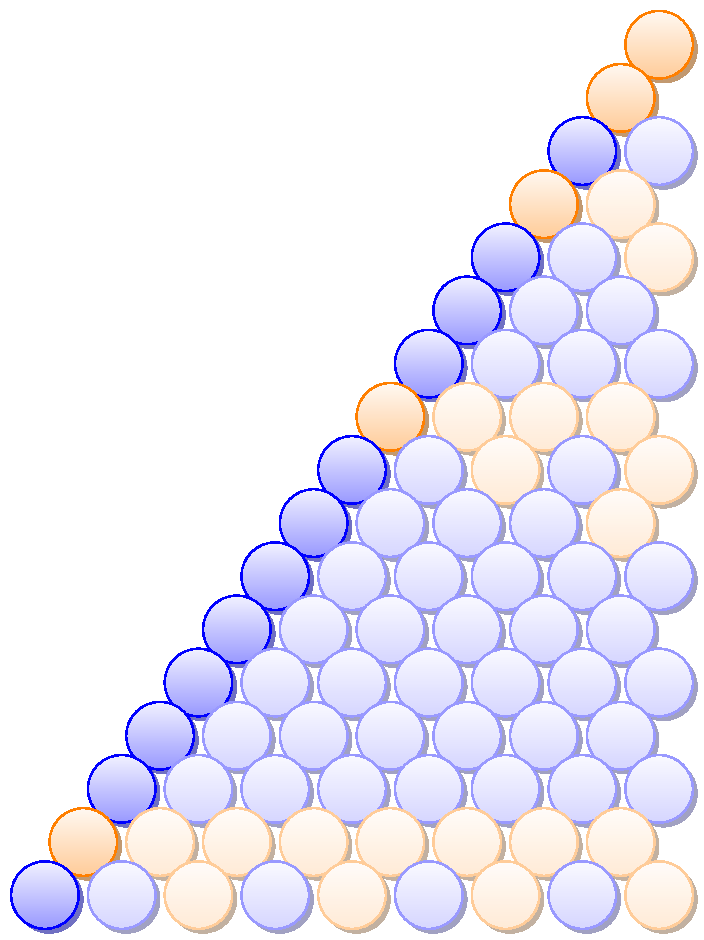
\includegraphics[
            width=7cm, 
            height=6cm, 
            keepaspectratio=true]{catalan-tikz/first-column/first-column.pdf}
    }

    % this 'particular' line is necessary to use `displaymath' environment
    % into the caption environment, togheter with the inclusion of 
    % `caption' package. See here for more explanation:
    % http://stackoverflow.com/questions/2716227/adding-an-equation-or-formula-to-a-figure-caption-in-latex
    \captionsetup{singlelinecheck=off}
    \caption[.]{ \textcolor{blue}{even},
        \textcolor{orange}{odd}  }

    \label{fig:catalan-first-column}

\end{figure}


\subsection{On rows composed of \emph{odd} coeffients only}

\begin{theorem}
    Every row $\vect{r}_{2^{\alpha}-1}$ of $\mathcal{C}_{\equiv_{2}}$, 
    for $\alpha\in\mathbb{N}$, is composed of \emph{odd} coefficients only.
\end{theorem}

\begin{proof}
    Choose any $\alpha\in\mathbb{N}$. For the very first coefficient $d_{2^{\alpha}-1,0}$ 
    lying on row $\vect{r}_{2^{\alpha}-1}$ we have seen in the
    previous section that $d_{2^{\alpha}-1,0}\equiv_{2}1$. What about $d_{2^{\alpha}-1,1}$?
    Recall we can write it, according to 
    \autoref{eq:convolution:expansion:for:generic:element:in:catalan:array}, as:
    \begin{displaymath}
        d_{2^{\alpha}-1,1} = \sum_{i_{1}+ i_{2}=2^{\alpha}}{ c_{i_{1}-1}\,c_{i_{2}-1} }
    \end{displaymath}
    Summation constraints indices $i_{1}$ and $i_{2}$ such that 
    $2^{\alpha}$ divides $i_{1}+i_{2}$ \emph{exactly}, so:
    \begin{displaymath}
        1 = \frac{i_{1}}{2^{\alpha}}+\frac{i_{2}}{2^{\alpha}} \qquad 
            i_{1},i_{2}\in\lbrace 0,\ldots,2^{\alpha}\rbrace
    \end{displaymath}
    %, which is the same to say that 
    %$\frac{i_{1}}{2^{\alpha}}$ and $\frac{i_{2}}{2^{\alpha}}$ are both integers.
    This implies that there exists $\beta,\gamma\in\mathbb{N}$, where $\beta,\gamma\leq\alpha$,
    such that $i_{1}=2^{\beta}$ and $i_{2}=2^{\gamma}$, respectively.

    By this fact follows that $c_{i_{1}-1}=c_{2^{\beta}-1}\equiv_{2}1$ and 
    $c_{i_{2}-1}=c_{2^{\gamma}-1}\equiv_{2}1$, therefore $c_{i_{1}-1}\,c_{i_{2}-1}\equiv_{2}1$.
    By construction, fixing one index in  
    $i_{1}+ i_{2}=2^{\alpha}$ fixes the other as well: there are $2^{\alpha}+1$ available choices
    for the first index and only $1$ for the second.
    We're almost finished:
    \begin{displaymath}
        d_{2^{\alpha}-1,1} = \sum_{i_{1}+ i_{2}=2^{\alpha}}{ c_{i_{1}-1}\,c_{i_{2}-1} }
            \equiv_{2} \sum_{k=1}^{2^{\alpha}+1}{1}\equiv_{2} 2^{\alpha}+1\equiv_{2} 1
    \end{displaymath}

    What about for an arbitrary coefficient $d_{2^{\alpha}-1,s}$ where
    $s\in\lbrace{2,\ldots,2^{\alpha}-1}\rbrace$?  Again, rewrite it as:
    \begin{displaymath}
        d_{2^{\alpha}-1,s} = \sum_{i_{1}+i_{2}+\ldots+i_{s+1}=2^{\alpha}}
            {c_{i_{1}-1}\,c_{i_{2}-1}\ldots\,c_{i_{s+1}-1}}
    \end{displaymath}
    Using an argument similar to the previous one, from:
    \begin{displaymath}
        1 = \frac{i_{1}}{2^{\alpha}}+\ldots+\frac{i_{s+1}}{2^{\alpha}} \qquad 
            i_{j}\in\lbrace 0,\ldots,2^{\alpha}\rbrace
    \end{displaymath} 
    the generic index $i_{j}$ has to satisfy $i_{j}=2^{\alpha_{j}}$, for some
    $\alpha_{j}\leq\alpha$. Therefore $c_{i_{j}-1}\equiv_{2}1$,
    for $j\in\lbrace1,\ldots,s+1\rbrace$, so:
    \begin{displaymath}
        d_{2^{\alpha}-1,s} \equiv_{2} \sum_{i_{1}+i_{2}+\ldots+i_{s+1}=2^{\alpha}}{1}
            \equiv_{2} {{s+2^{\alpha}}\choose{2^{\alpha}}}
    \end{displaymath}
    because the summation over indices $i_{1},\ldots,i_{s+1}$ asks to count the
    number of $2^{\alpha}$-combinations of $s+1$ distinct objects, each of
    which may appear indefinitely often, that is, $0$ to $2^{\alpha}$ times:
    the saught number is ${{(s+1)+2^{\alpha}-1}\choose{2^{\alpha}}}$
    (see \cite{riordan:intro:combinatorial:analysis}, pag. 7, equation 10).

    Again, we're interested on the parity of such coefficient, therefore
    write $s=s_{0}+s_{1}\,2+\ldots+s_{\alpha-1}\,2^{\alpha-1}$, because $s$ can equal 
    $2^{\alpha}-1$ at most, and apply Lucas theorem one more time:
    \begin{displaymath}
        {{s+2^{\alpha}}\choose{2^{\alpha}}}\equiv_{2} 
            {{s_{0}}\choose{0}}{{s_{1}}\choose{0}} \ldots
                {{s_{\alpha-1}}\choose{0}}{{1}\choose{1}}\equiv_{2}1 
    \end{displaymath}
    the general case holds too, therefore each coefficient lying on
    a row $\vect{r}_{2^{\alpha}-1}$ is odd, as required.
\end{proof}


\begin{figure}[p]

    \noindent\makebox[\textwidth]{
        \centering
        %\includegraphics[width=0.8\textwidth]{../../sympy/catalan/coloured.pdf}

        % using *angle* property to rotate it is difficult to properly align it
        % in order to have a "real" matrix representation.
        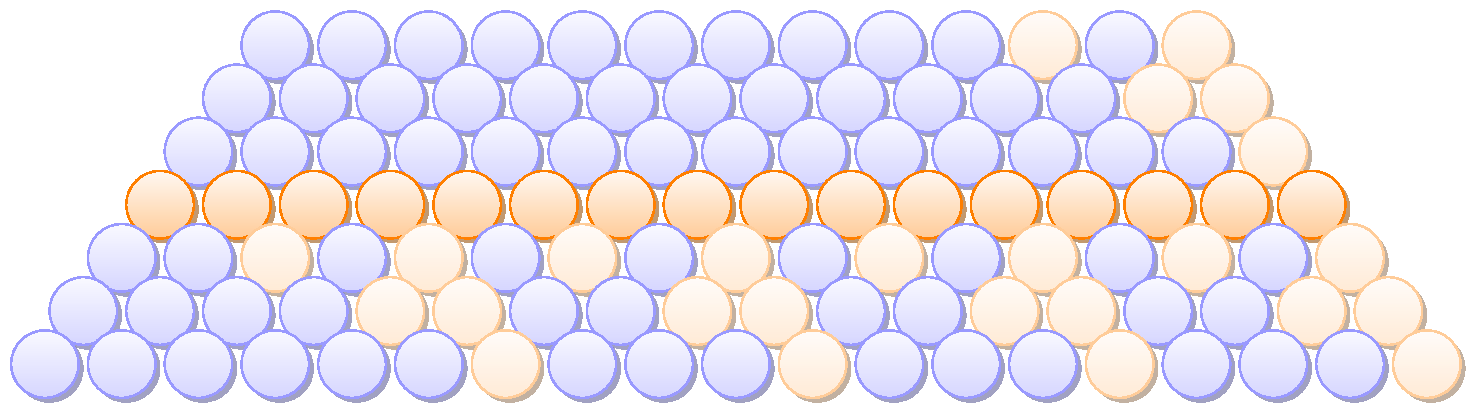
\includegraphics[width=10cm, height=10cm, keepaspectratio=true]
            {../RART2015/catalan-tikz/odd-row/odd-row.pdf}
    }

    % this 'particular' line is necessary to use `displaymath' environment
    % into the caption environment, togheter with the inclusion of 
    % `caption' package. See here for more explanation:
    % http://stackoverflow.com/questions/2716227/adding-an-equation-or-formula-to-a-figure-caption-in-latex
    \captionsetup{singlelinecheck=off}
    \caption[Row $\vect{r}_{2^{4}-1}$ of $\mathcal{C}_{\equiv_{2}}$]{
        Row $\vect{r}_{2^{4}-1}$ composed of coefficients $\textcolor{orange}{d_{2^{4}-1,s} \equiv_{2} 1}$, 
        for $s\in\lbrace1,\ldots,2^{4}-1 \rbrace$ }

    \label{fig:catalan-odd-row}

\end{figure}

In \autoref{fig:catalan-odd-row} row $\vect{r}_{2^{4}-1}$ is highlighted.

\subsection{On rows composed of odd and even coefficients}

\begin{theorem}
    Let $\vect{r}_{2^{\alpha}}$ be a row of $\mathcal{C}_{\equiv_{2}}$, 
    for some $\alpha\in\mathbb{N}$. Then, excluded the very first coefficient 
    $d_{2^{\alpha},0}$, which is even, $\vect{r}_{2^{\alpha}}$ is composed of
    alternating even and odd coefficients. Formally:
    \begin{displaymath}
        d_{2^{\alpha},j}\equiv_{2}0 \leftrightarrow j = 2k+1
    \end{displaymath}
    for some $k\in\mathbb{N}$.
\end{theorem}

\begin{proof}
    Let $d_{2^{\alpha},j}$ be a coefficient lying on row $\vect{r}_{2^{\alpha}}$,
    for some $j\in\lbrace1,\ldots,2^{\alpha}\rbrace$.

    Since $\mathcal{C}$'s $A$-sequence is:
    \begin{displaymath}
        A_{\mathcal{C}}(t)=\frac{1}{1-t}=1+t+t^{2}+t^{3}+t^{4}+t^{5}+t^{6}+t^{7}+t^{8}+
            \mathcal{O}(t^{9})
    \end{displaymath}
    it follows that $d_{2^{\alpha},j}$ can be written as the combination of $r+2$
    coefficients lying on the previous row, namely $\vect{r}_{2^{\alpha}-1}$:
    \begin{displaymath}
        d_{2^{\alpha},j} = d_{2^{\alpha}-1,j-1} +d_{2^{\alpha}-1,j} +\ldots+d_{2^{\alpha}-1,j+r} 
    \end{displaymath}
    where $r$ satisfies $r=2^{\alpha}-1-j$, so $2^{\alpha}-j+1$ coefficients are 
    combined.  By     the theorem above, row $\vect{r}_{2^{\alpha}-1}$ is composed by \emph{odd}
    coefficients only, therefore proceed by cases on the parity of $j$:
    \begin{itemize}
        \item if $j$ is \emph{odd}, assume $j=2k+1$ for some $k\in\mathbb{N}$, then
            $2^{\alpha}-2k$ coefficients are combined, which is an \emph{even} number. 
            Adding an \emph{even} number of \emph{odd} numbers yield an \emph{even} number;
        \item if $j$ is \emph{even}, assume $j=2k$ for some $k\in\mathbb{N}$, then
            $2^{\alpha}-2k+1$ coefficients are combined, which is an \emph{odd} number. 
            Adding an \emph{odd} number of \emph{odd} numbers yield an \emph{odd} number.
    \end{itemize}
\end{proof}


\begin{figure}[p]

    \noindent\makebox[\textwidth]{
        \centering
        %\includegraphics[width=0.8\textwidth]{../../sympy/catalan/coloured.pdf}

        % using *angle* property to rotate it is difficult to properly align it
        % in order to have a "real" matrix representation.
        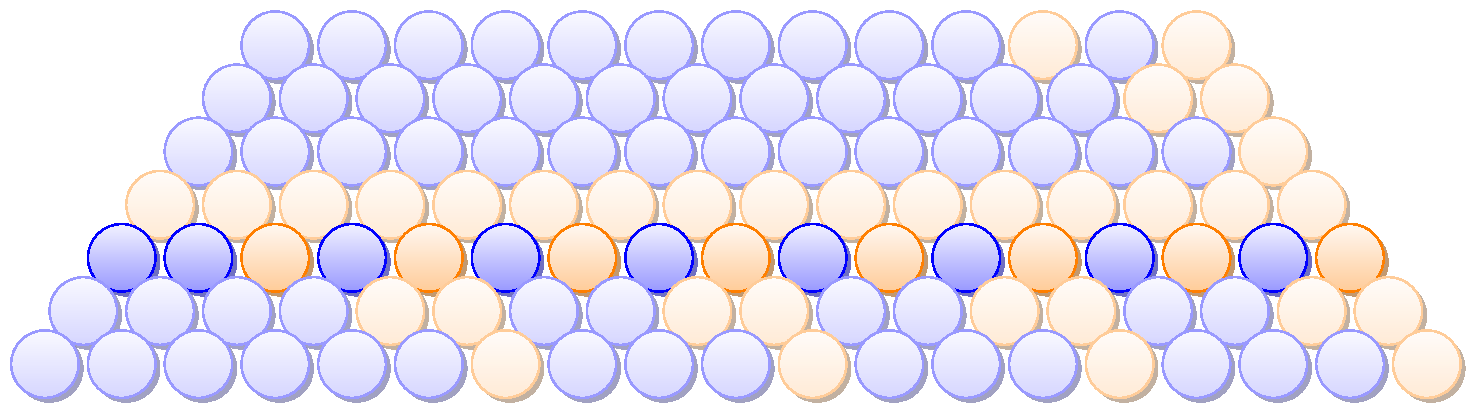
\includegraphics[width=10cm, height=3cm, keepaspectratio=true]{catalan-tikz/odd-row/alternating-row.pdf}
    }

    % this 'particular' line is necessary to use `displaymath' environment
    % into the caption environment, togheter with the inclusion of 
    % `caption' package. See here for more explanation:
    % http://stackoverflow.com/questions/2716227/adding-an-equation-or-formula-to-a-figure-caption-in-latex
    \captionsetup{singlelinecheck=off}
    \caption[.]{Row of coefficients $\textcolor{orange}{d_{2^{4}-1,s}} \equiv_{2} 1$ 
        for $s\in\lbrace1,\ldots,2^{4}-1 \rbrace$ }

    \label{fig:catalan-odd-row}

\end{figure}

In \autoref{fig:catalan-alternating-row} row $\vect{r}_{2^{4}}$ is highlighted.

\subsection{On the \flqq mirror\frqq\, segment}

Before showing new theorems, we introduce the object
$\Phi^{(\alpha)}$ which denotes a particular segment contained 
in the principal cluster $\mathcal{C}^{(\alpha+1)}$. 
We call $\Phi^{(\alpha)}$ the \flqq mirror\frqq\,segment in 
$\mathcal{C}^{(\alpha+1)}$ and it is defined as follows:
\begin{displaymath}
    \Phi^{(\alpha)}=\diagup_{\lbrace 1,2,\ldots,2^{\alpha}-1\rbrace}^{2^{\alpha}-1}
\end{displaymath}

\begin{theorem}
    Choose any $\alpha\in\mathbb{N}$, then $\Phi^{(\alpha)}$ satisfies: 
    \begin{displaymath}
        d_{s,2^{\alpha}-1}\in\Phi^{(\alpha)} \rightarrow d_{s,2^{\alpha}-1}\equiv_{2}0
    \end{displaymath}
    where $s\in rows\left(\Phi^{(\alpha)}\right)=\lbrace2^{\alpha},\ldots,2^{\alpha+1}-2\rbrace$.
\end{theorem}

\begin{proof}
Let $d_{s,2^{\alpha}-1}$ a coefficient in the segment $\Phi^{(\alpha)}$, 
according to \autoref{eq:convolution:expansion:for:generic:element:in:catalan:array} 
write it as:
\begin{displaymath}
    d_{s, 2^{\alpha}-1} = \sum_{i_{1}+i_{2}+\ldots+i_{2^{\alpha}}=s+1}
        {c_{i_{1}-1}\,c_{i_{2}-1}\ldots\,c_{i_{2^{\alpha}}-1}}
\end{displaymath}
Observe that, for $s$ varing in the allowed range of $\Phi^{(\alpha)}$,
the number of Catalan coefficients
multiplied together in each summand is the same, namely $2^{\alpha}$. 
What changes respect to $s$ is the set of values 
each index $i_{j}$ can take. Look at the following table, where $j$ and $k$
are dummy variables:
\begin{displaymath}
    \begin{array}{c|c|c}
        s = 2^{\alpha} 
            & i_{j}\in\lbrace0,\ldots,2^{\alpha}+1\rbrace 
            & c_{k}\in\lbrace c_{-1},\ldots,c_{2^{\alpha}}\rbrace\\
        s = 2^{\alpha} +1
            & i_{j}\in\lbrace0,\ldots,2^{\alpha}+2\rbrace 
            & c_{k}\in\lbrace c_{-1},\ldots,c_{2^{\alpha}+1}\rbrace\\
        \vdots & \vdots&\vdots \\
        s = 2^{\alpha+1} -2
            & i_{j}\in\lbrace0,\ldots,2^{\alpha+1}-1\rbrace 
            & c_{k}\in\lbrace c_{-1},\ldots,c_{2^{\alpha+1}-2}\rbrace\\
    \end{array}
\end{displaymath}
observe that set $\lbrace c_{-1},\ldots,c_{2^{\alpha}}\rbrace$, the smaller one, and set
$\lbrace c_{-1},\ldots,c_{2^{\alpha+1}-2}\rbrace$, the bigger one, have the same subset
$\Omega^{(\alpha)}$ of \emph{odd} coefficients: 
\begin{displaymath}
    \Omega^{(\alpha)}=\lbrace c_{-1}, c_{2^{\alpha-(\alpha-1)}-1},c_{2^{\alpha-(\alpha-2)}-1},\ldots, 
        c_{2^{\alpha-1}-1},c_{2^{\alpha}-1}\rbrace
\end{displaymath}
where $\left|\Omega^{(\alpha)}\right|=\alpha+1$.
Since each summand term $c_{i_{1}-1}\,c_{i_{2}-1}\ldots\,c_{i_{2^{\alpha}}-1}$ 
has $2^{\alpha}$ coefficients, no matter if it contains each coefficient in $\Omega^{(\alpha)}$ and,
more importantly, one of them cannot belong to $\Omega^{(\alpha)}$:
the remaining ones make it vanish and $d_{s, 2^{\alpha}-1} \equiv_{2} 0$, for any suitable $s$,
as required.

\end{proof}


\begin{figure}[htb]

    \noindent\makebox[\textwidth]{
        \centering
        %\includegraphics[width=0.8\textwidth]{../../sympy/catalan/coloured.pdf}

        % using *angle* property to rotate it is difficult to properly align it
        % in order to have a "real" matrix representation.
        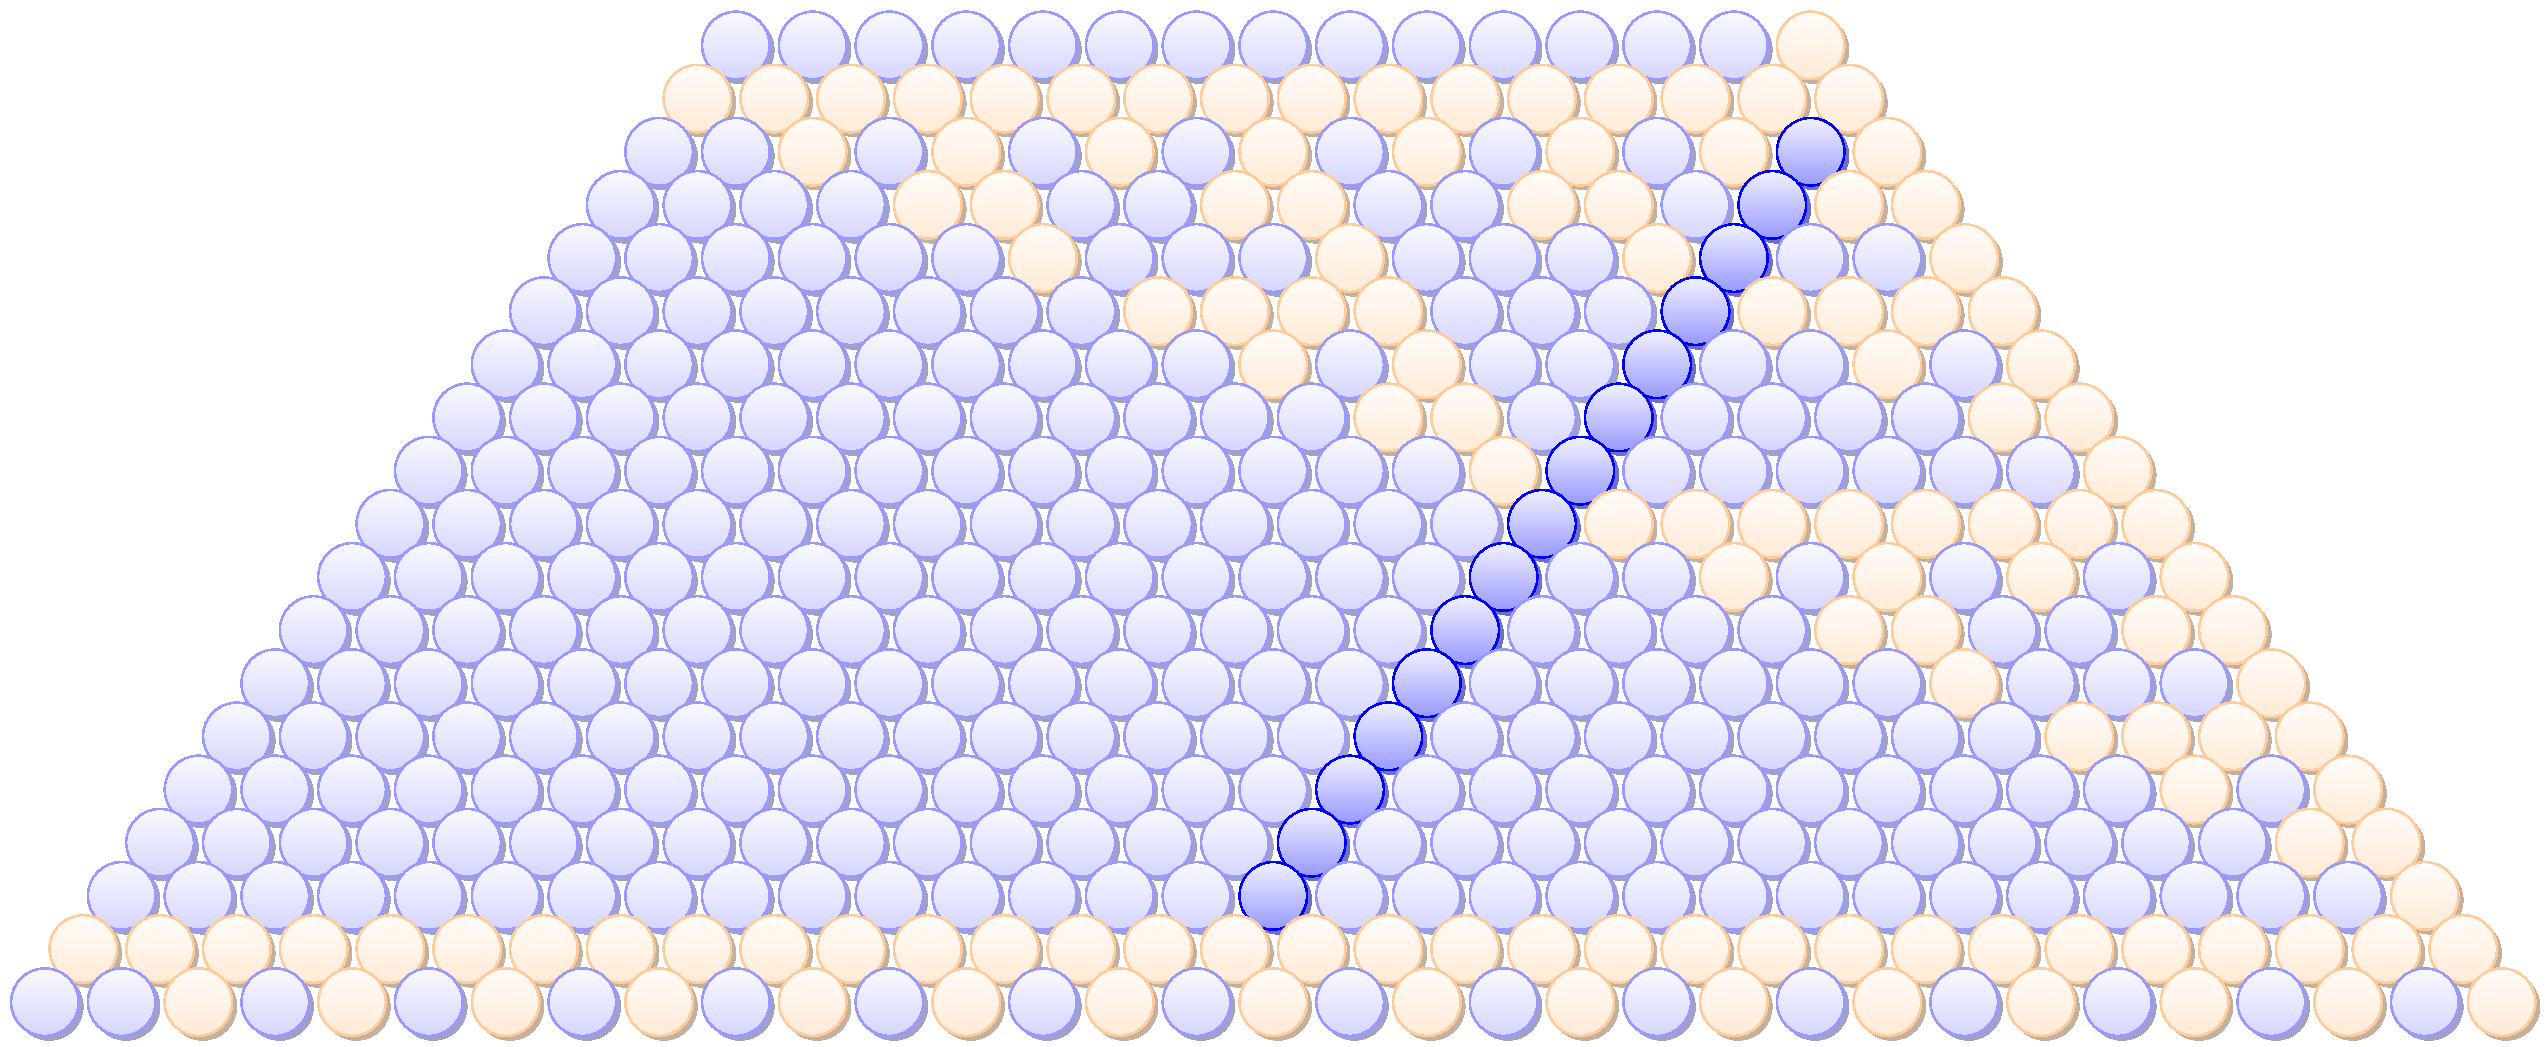
\includegraphics[width=10cm, height=10cm, keepaspectratio=true]
            {../RART2015/catalan-tikz/mirror-segment/mirror-segment.pdf}
    }

    % this 'particular' line is necessary to use `displaymath' environment
    % into the caption environment, togheter with the inclusion of 
    % `caption' package. See here for more explanation:
    % http://stackoverflow.com/questions/2716227/adding-an-equation-or-formula-to-a-figure-caption-in-latex
    \captionsetup{singlelinecheck=off}
    \caption[\emph{Mirror} segment $\Phi^{(4)}$ in $\mathcal{C}_{\equiv_{2}}^{(5)}$]
        {\emph{Mirror} segment $\Phi^{(4)}=\diagup_{\lbrace 1,2,\ldots,2^{4}-1\rbrace}^{2^{4}-1}$
        in $\mathcal{C}_{\equiv_{2}}^{(5)}$ }

    \label{fig:mirror-segment}

\end{figure}

In \autoref{fig:mirror-segment} the \flqq mirror\frqq\,segment $\Phi^{(4)}$ is highlighted.

\subsection{On the \flqq dual\frqq\,segment of the \flqq mirror\frqq\, segment}

Next theorem needs a new piece of notation that allows us to identify a 
new portion within a principal cluster $\mathcal{C}^{(\alpha+1)}$.
Let $\hat{\Phi}^{(\alpha)}$ denote the set $\left\lbrace d_{s,s-(2^{\alpha}-1)}\right\rbrace$,
for $s\in rows\left(\Phi^{(\alpha)}\right)$: we call $\hat{\Phi}^{(\alpha)}$  
the \flqq dual\frqq\, segment of the \flqq mirror\frqq\,segment $\Phi^{(\alpha)}$.

\begin{theorem}
    Let  $\Phi^{(\alpha)}=\diagup_{\lbrace 1,2,\ldots,2^{\alpha}-1\rbrace}^{2^{\alpha}-1}$, 
    be a \flqq mirror\frqq\,segment in $\mathcal{C}^{(\alpha+1)}$, then: 
    \begin{equation}
        d_{s,2^{\alpha}-1}\in\Phi^{(\alpha)}\rightarrow d_{s,s-(2^{\alpha}-1)}\equiv_{2}d_{s,2^{\alpha}-1}
    \end{equation}
    where $s\in rows\left(\Phi^{(\alpha)}\right)=\lbrace2^{\alpha},\ldots,2^{\alpha+1}-2\rbrace$.
\end{theorem}

\begin{proof}
    Use \autoref{eq:catalan:array:second:identity} on both members:
    \begin{displaymath}
        {{s+2^{\alpha}-1}\choose{2^{\alpha}-1}}- {{s+2^{\alpha}-1}\choose{2^{\alpha}-2}} \equiv_{2}
        {{2s-2^{\alpha}+1}\choose{s-2^{\alpha}+1}}- {{2s-2^{\alpha}+1}\choose{s-2^{\alpha}}}
    \end{displaymath}
    by symmetry property of binomial coefficients:
    \begin{displaymath}
        {{s+2^{\alpha}-1}\choose{s}}- {{s+2^{\alpha}-1}\choose{s+1}} \equiv_{2}
        {{2s-2^{\alpha}+1}\choose{s}}- {{2s-2^{\alpha}+1}\choose{s+1}}
    \end{displaymath}
    by simplification using $(-1)^{-1}\mod 2=1$: 
    \begin{displaymath}
        {{s+2^{\alpha}-1}\choose{s}}+ {{s+2^{\alpha}-1}\choose{s+1}} \equiv_{2}
        {{2s-2^{\alpha}+1}\choose{s}}+ {{2s-2^{\alpha}+1}\choose{s+1}}
    \end{displaymath}
    by classic recurrence rule of binomial coefficients:
    \begin{displaymath}
        {{s+2^{\alpha}}\choose{s+1}} \equiv_{2} {{2s-2^{\alpha}+2}\choose{s+1}}
    \end{displaymath}
    since $s$ can assume $2^{\alpha}$ at least and $2^{\alpha+1}-2$ at most, 
    $s$ can be written in base $2$ as follows:
    \begin{displaymath}
        s=s_{0} + s_{1}2 + s_{2}2^{2}+\ldots+s_{\alpha-1}2^{\alpha-1}+2^{\alpha}
    \end{displaymath}
    and applying Lucas theorem we get:

    \begin{displaymath}
        \hspace{-2cm}
        {{s_{0}}\choose{s_{0}+1}}
        {{s_{1}}\choose{s_{1}}}
        \ldots
        {{s_{\alpha-1}}\choose{s_{\alpha-1}}}
        {{0}\choose{1}}
        {{1}\choose{0}}
        \equiv_{2}
        {{0}\choose{s_{0}+1}}
        {{s_{0}+1}\choose{s_{1}}}
        {{s_{1}}\choose{s_{2}}}
        \ldots
        {{s_{\alpha-2}}\choose{s_{\alpha-1}}}
        {{s_{\alpha-1}-1}\choose{1}}
        {{1}\choose{0}}
    \end{displaymath}
    simple algebra:
    \begin{displaymath}
        0
        \equiv_{2}
        {{0}\choose{s_{0}+1}}
        {{s_{0}+1}\choose{s_{1}}}
        {{s_{1}}\choose{s_{2}}}
        \ldots
        {{s_{\alpha-2}}\choose{s_{\alpha-1}}}
        {{s_{\alpha-1}-1}\choose{1}}
    \end{displaymath}
    %\marginpar{in order to finish this proof we have to introduce a lemma about
    %    the row of alternating odd and even coefficient, which can be proved using
    %    the $A$-sequence of $\mathcal{C}$}
    By cases on the parity of $s$:
    \begin{itemize}
        \item assume $s$ is \emph{even}, therefore $s_{0}=0$ and the right hand side vanishes due to ${{0}\choose{s_{0}+1}}=0$;
        \item assume $s$ is \emph{odd}, therefore $s_{0}=1$, so apply Lucas theorem to ${{0}\choose{2}}$ again,
            yielding ${{0}\choose{2}}\equiv_{2}{{0}\choose{0}}{{0}\choose{1}}\equiv_{2}0$.
    \end{itemize}
    both cases shows that right hand side is a multiple of $p$, as required.
\end{proof}


\begin{figure}[p]

    \noindent\makebox[\textwidth]{
        \centering
        %\includegraphics[width=0.8\textwidth]{../../sympy/catalan/coloured.pdf}

        % using *angle* property to rotate it is difficult to properly align it
        % in order to have a "real" matrix representation.
        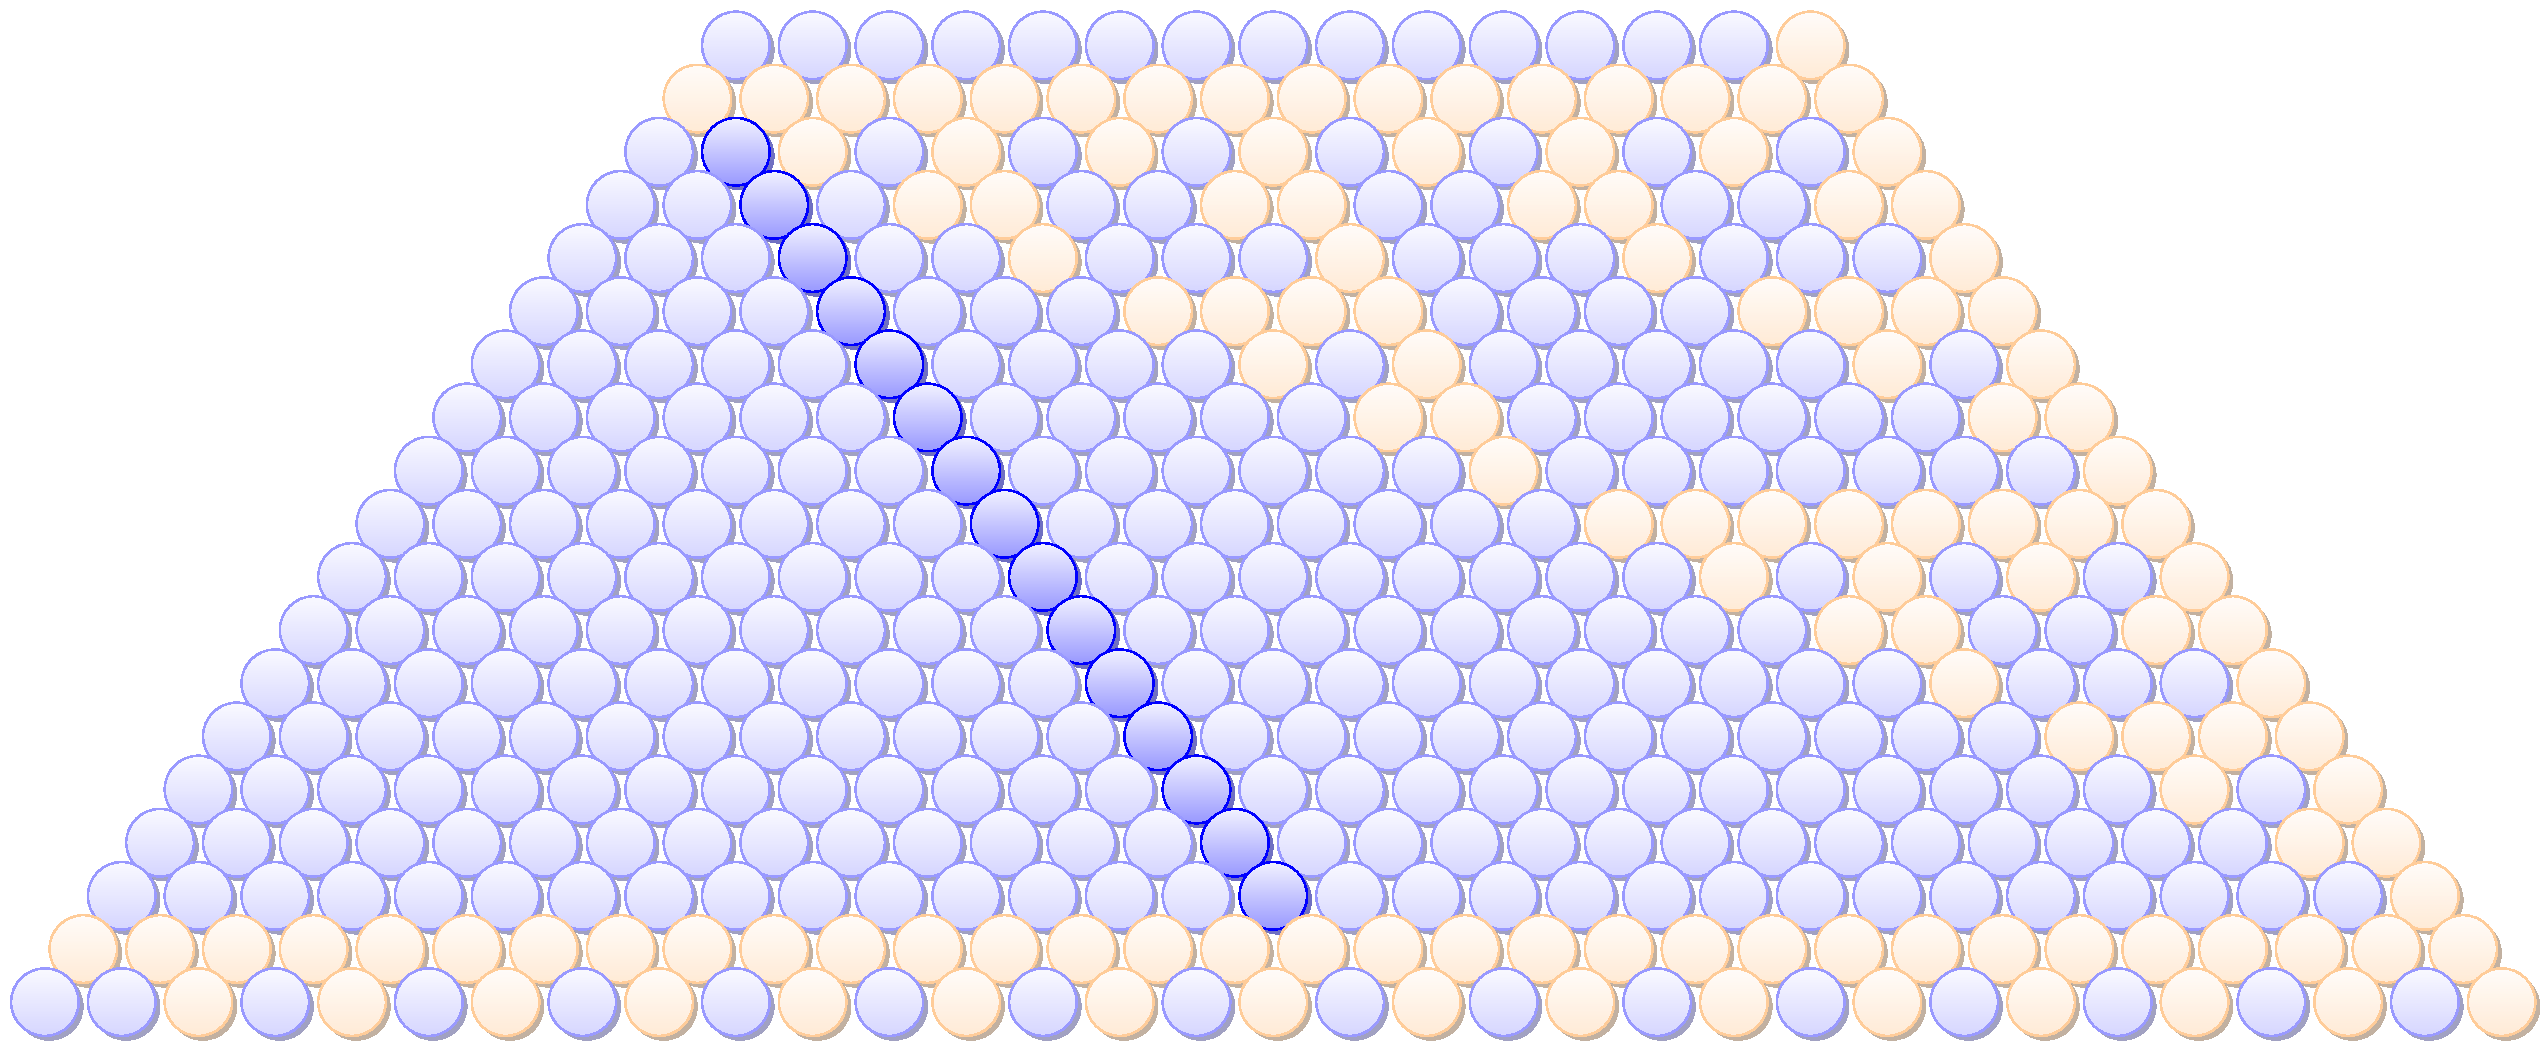
\includegraphics[width=10cm, height=10cm, keepaspectratio=true]
            {../RART2015/catalan-tikz/dual-of-mirror-segment/dual-of-mirror-segment.pdf}
    }

    % this 'particular' line is necessary to use `displaymath' environment
    % into the caption environment, togheter with the inclusion of 
    % `caption' package. See here for more explanation:
    % http://stackoverflow.com/questions/2716227/adding-an-equation-or-formula-to-a-figure-caption-in-latex
    \captionsetup{singlelinecheck=off}
    \caption[\emph{Dual} segment $\left\lbrace d_{s,s-(2^{4}-1)}\right\rbrace$,
        for $s\in rows\left(\Phi^{(4)}\right)$, in $\mathcal{C}_{\equiv_{2}}^{(5)}$]
        { \emph{Dual} segment $\left\lbrace d_{s,s-(2^{4}-1)}\right\rbrace$,
                for $s\in rows\left(\Phi^{(4)}\right)$, of \emph{mirror} segment $\Phi^{(4)}$ }



    \label{fig:dual-of-mirror-segment}

\end{figure}

In \autoref{fig:dual-of-mirror-segment} the \flqq dual\frqq\,segment 
    $\left\lbrace d_{s,s-(2^{4}-1)}\right\rbrace$,
    for $s\in rows\left(\Phi^{(4)}\right)$, of \flqq mirror\frqq\,segment 
    $\Phi^{(4)}$ in $\mathcal{C}_{\equiv_{2}}^{(5)}$ is highlighted.

\subsection{On the \emph{upside-down} zero-hole}

\begin{theorem}
    Let $\mathcal{C}_{\equiv_{2}}^{(\alpha+1)}$ be a principal cluster 
    of order $\alpha+1$ of the Catalan array $\mathcal{C}$. Then, 
    $H_{\bigtriangleup}^{({\alpha})}$ denotes an \emph{upside-down} zero-hole of order $\alpha$,
    such that coefficient $d_{nk}\in H_{\bigtriangleup}^{({\alpha})}$ if 
    $n\in\lbrace 2^{{\alpha}},\ldots,2^{{\alpha}+1}-2\rbrace$ and 
    $k\in\lbrace 0,\ldots, n-2^{{\alpha}}\rbrace$. 
\end{theorem}

It is simple to observe that $H_{\bigtriangleup}^{({\alpha})}\subset
\mathcal{C}_{\equiv_{2}}^{(\alpha+1)}$. 

\begin{proof}
We repeatedly use the approach
of the proof about the \flqq mirror\frqq\,segment, considering the set of columns 
$\Xi=\lbrace \vect{c}_{0},\ldots, \vect{c}_{2^{{\alpha}}-2}\rbrace$ and
for each column $\vect{c}_{k}\in\Xi$, the segment
    $\diagup_{\lbrace 2^{\alpha},2^{\alpha}+1,\ldots,2^{\alpha+1}-2-k\rbrace}^{k}$.

Everything is set, so start from column on the very left, column $\vect{c}_{0}$.
So the corresponding set of row indices  is a segment of Catalan numbers:
\begin{displaymath}
    S_{0}=\diagup_{\lbrace 2^{\alpha},2^{\alpha}+1,\ldots,2^{\alpha+1}-2\rbrace}^{0}
        = \lbrace c_{2^{\alpha}},c_{2^{\alpha}+1},\ldots,c_{2^{\alpha+1}-2}\rbrace
\end{displaymath}
since no coefficient $c_{j}\in S_{0}$ has the shape $c_{2^{\alpha}-1}$, 
all coefficients in $S_{0}$ are even.

Go ahead with column $\vect{c}_{1}$, so the corresponding segment is :
\begin{displaymath}
    S_{1}=\diagup_{\lbrace 2^{\alpha},2^{\alpha}+1,\ldots,2^{\alpha+1}-3\rbrace}^{1}
    %S_{1}=\lbrace d_{2^{{\alpha}}+1,1},\ldots,d_{2^{{\alpha}+1}-2,1} \rbrace
\end{displaymath}
and coefficients in it are defined according to:
\begin{displaymath}
    d_{s, 1} = \sum_{i_{1}+i_{2}=s+1} {c_{i_{1}-1}\,c_{i_{2}-1}}
\end{displaymath}
where $s\in rows(S_{1})= \left\lbrace 2^{\alpha}+1,2^{\alpha}+2,\ldots,2^{\alpha+1}-2\right\rbrace$. 
This is quite similar to the proof developed for the \flqq mirror\frqq\,segment,
with the difference that summand term is composed of two coefficients, namely
$c_{i_{1}-1}\,c_{i_{2}-1}$ instead of $2^{{\alpha}}$ coefficients as in the previous proof, 
therefore the same argument applies,
since if multiplying $2^{{\alpha}}$ coefficients fails to make \emph{not} vanish
the summand term, modulo $2$, the same failure is reached if multiplying only $2$ coefficients.

The same reasoning holds for remaining columns in $\Xi$: the last one of them is 
$\vect{c}_{2^{\alpha}-2}$ (with only \emph{one} coefficient, namely $d_{2^{\alpha}-2,2^{\alpha}-2}$), 
hence $H_{\bigtriangleup}^{({\alpha})}$ is an \emph{upside-down} zero-holes of order $\alpha$,
positioned at the very left in the bottom half of $\mathcal{C}_{\equiv_{2}}^{(\alpha+1)}$, as required.

\end{proof}


\begin{figure}[p]

    \noindent\makebox[\textwidth]{
        \centering
        %\includegraphics[width=0.8\textwidth]{../../sympy/catalan/coloured.pdf}

        % using *angle* property to rotate it is difficult to properly align it
        % in order to have a "real" matrix representation.
        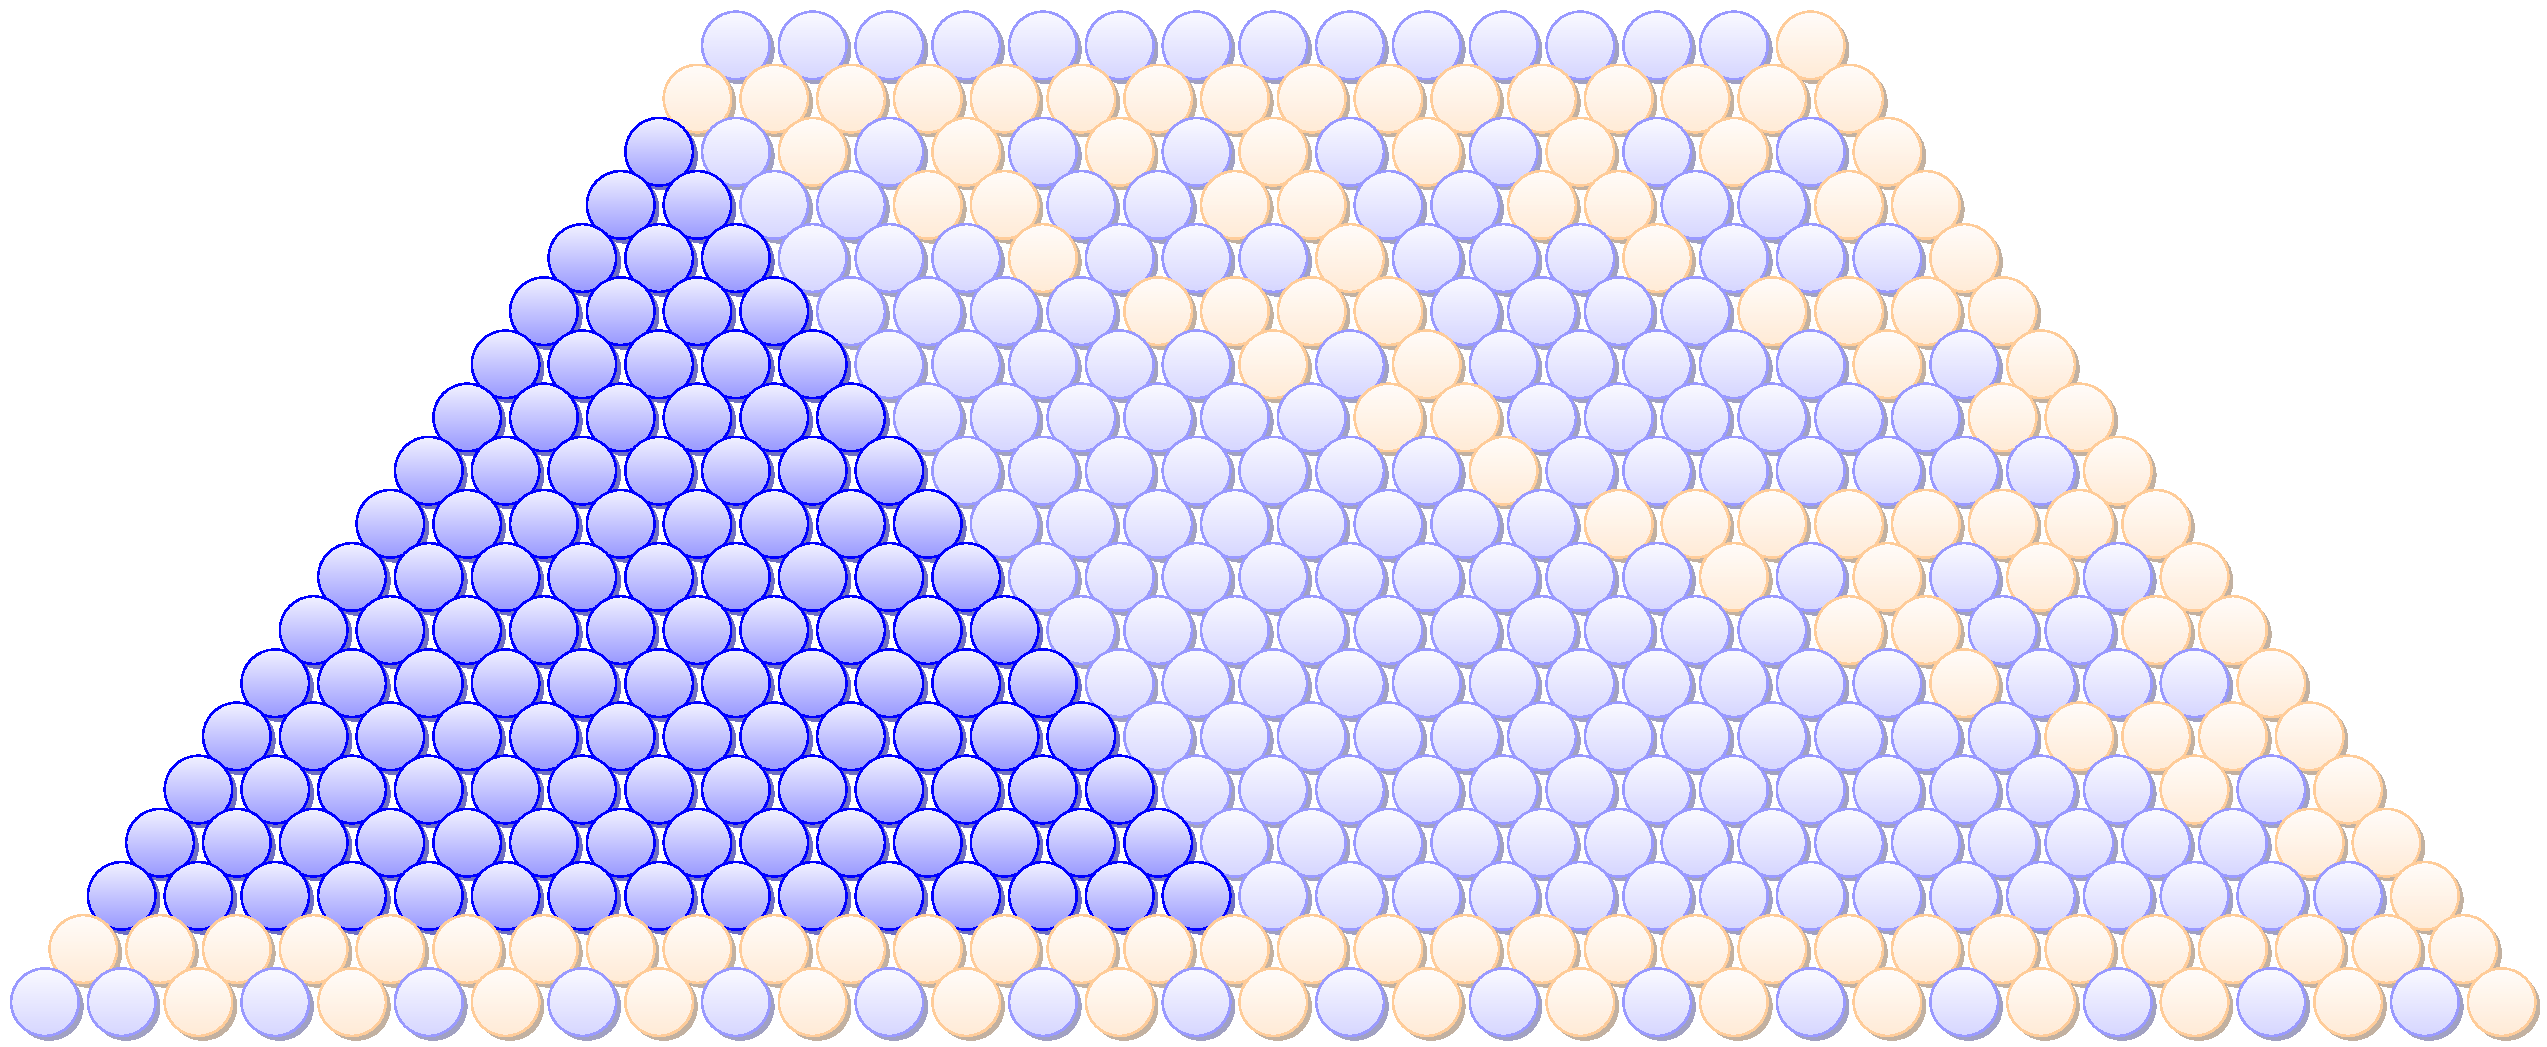
\includegraphics[width=10cm, height=10cm, keepaspectratio=true]
            {../RART2015/catalan-tikz/zero-hole/zero-hole.pdf}
    }

    % this 'particular' line is necessary to use `displaymath' environment
    % into the caption environment, togheter with the inclusion of 
    % `caption' package. See here for more explanation:
    % http://stackoverflow.com/questions/2716227/adding-an-equation-or-formula-to-a-figure-caption-in-latex
    \captionsetup{singlelinecheck=off}
    \caption[Upside-down zero-hole $T_{\bigtriangleup}^{(4)}$ within
        $\mathcal{C}_{\equiv_{2}}^{(\alpha+1)}$]{Zero hole $T_{\bigtriangleup}^{(4)} \subset \mathcal{C}_{\equiv_{2}}^{(5)}$}

    \label{fig:catalan-zero-hole}

\end{figure}

In \autoref{fig:catalan-zero-hole} is reported $H_{\bigtriangleup}^{(4)}$.

\subsection{On two \flqq mirrored\frqq\,clusters}

\begin{theorem}
    Let $\Phi^{(\alpha)}=\diagup_{\lbrace 2,\ldots,2^{\alpha}-1\rbrace}^{2^{\alpha}-1}$
    be a \flqq mirror\frqq\,segment and $\hat{d}_{s,2^{{\alpha}}-1}$ 
    be a coefficient in $\Phi^{(\alpha)}$, for some $s\in rows\left(\Phi^{(\alpha)}\right)$. Then:
    \begin{displaymath}
        d_{s-e,2^{{\alpha}}-1-e} \equiv_{2} d_{s,2^{{\alpha}}-1+e}
    \end{displaymath}
    for $e\in\lbrace1,\ldots,s-2^{{\alpha}}\rbrace$.
\end{theorem}

Before approaching a structured proof, we look for some insights.
According to \autoref{eq:convolution:expansion:for:generic:element:in:catalan:array},
rewrite both members:
\begin{displaymath}
    \hspace{-2cm}
    \sum_{i_{1}+i_{2}+\ldots+i_{2^{\alpha}-e}=s-e+1}
        {c_{i_{1}-1}\,c_{i_{2}-1}\ldots\,c_{i_{2^{\alpha}-e}-1}}
    \equiv_{2}
    \sum_{i_{1}+i_{2}+\ldots+i_{2^{\alpha}+e}=s+1}
        {c_{i_{1}-1}\,c_{i_{2}-1}\ldots\,c_{i_{2^{\alpha}+e}-1}}
\end{displaymath}
panic! No idea to tackle the general setting as a whole. So, start small and
let $s=2^{{\alpha}}+1$, therefore no choices for $e$, $e=1$ is mandatory:
\begin{displaymath}
    \hspace{-2cm}
    \sum_{i_{1}+i_{2}+\ldots+i_{2^{\alpha}-1}=2^{{\alpha}}+1}
        {c_{i_{1}-1}\,c_{i_{2}-1}\ldots\,c_{i_{2^{\alpha}-1}-1}}
    \equiv_{2}
    \sum_{i_{1}+i_{2}+\ldots+i_{2^{\alpha}+1}=2^{{\alpha}}+2}
        {c_{i_{1}-1}\,c_{i_{2}-1}\ldots\,c_{i_{2^{\alpha}+1}-1}}
\end{displaymath}

too difficult to proceed on this path, too. 

We attempt another \emph{false start} using closed formulae for
the generic element $d_{nk}\in\mathcal{C}$.
\begin{proof}
Assume not, therefore we need to yield a contraddiction if:
\begin{displaymath}
    d_{s-e,2^{{\alpha}}-1-e} \not\equiv_{2} d_{s,2^{{\alpha}}-1+e}
\end{displaymath}
holds. Rewriting the congruence according to \autoref{eq:catalan:array:first:identity}
 for $d_{nk}$:
\begin{displaymath}
    \frac{2^{{\alpha}}-e}{s-e+1}{{2(s-e)-(2^{{\alpha}}-1-e)}\choose{s-e-(2^{{\alpha}}-1-e)}}
    \not\equiv_{2}
    \frac{2^{{\alpha}}+e}{s+1}{{2s-(2^{{\alpha}}-1+e)}\choose{s-(2^{{\alpha}}-1+e)}}
\end{displaymath}
simplify it:
\begin{displaymath}
    \frac{2^{{\alpha}}-e}{s-e+1}{{2s-e-2^{{\alpha}}+1}\choose{s-2^{{\alpha}}+1}}
    \not\equiv_{2}
    \frac{2^{{\alpha}}+e}{s+1}{{2s-2^{{\alpha}}+1-e}\choose{s-2^{{\alpha}}+1-e}}
\end{displaymath}
manipulate using ${{n}\choose{k}}={{n}\choose{n-k}}$:
\begin{displaymath}
    \frac{2^{{\alpha}}-e}{s-e+1}{{2s-e-2^{{\alpha}}+1}\choose{s-e}}
    \not\equiv_{2}
    \frac{2^{{\alpha}}+e}{s+1}{{2s-2^{{\alpha}}+1-e}\choose{s}}
\end{displaymath}
dead end: nonetheless binomial coeffients allow some grunging,
fractions on both side are difficult to handle since it's hard
to find their multiplicative inverses, modulo $2$. A contraddiction
is difficult to be reached using this approach.
\end{proof} 

Trace back and use \autoref{eq:catalan:array:second:identity}. 
\begin{proof}
Recall we would like to prove the following statement:
\begin{displaymath}
    d_{s-e,2^{{\alpha}}-1-e} \equiv_{2} d_{s,2^{{\alpha}}-1+e}
\end{displaymath}
Rewrite the left hand side:
\begin{displaymath}
    d_{s-e,2^{{\alpha}}-1-e}= {{2(s-e)-(2^{{\alpha}}-1-e)}\choose{(s-e)-(2^{{\alpha}}-1-e)}}
        - {{2(s-e)-(2^{{\alpha}}-1-e)}\choose{(s-e)-(2^{{\alpha}}-1-e)-1}}
\end{displaymath}
in the same spirit, rewrite the right hand side:
\begin{displaymath}
    d_{s,2^{{\alpha}}-1+e}={{2s-(2^{{\alpha}}-1+e)}\choose{s-(2^{{\alpha}}-1+e)}}
        - {{2s-(2^{{\alpha}}-1+e)}\choose{s-(2^{{\alpha}}-1+e)-1}}
\end{displaymath}
therefore:
\begin{displaymath}
    \begin{split}
        {{2s-e-2^{{\alpha}}+1}\choose{s-2^{{\alpha}}+1}}
            - {{2s-e-2^{{\alpha}}+1}\choose{s-2^{{\alpha}}}}
        &\equiv_{2}
        {{2s-2^{{\alpha}}+1-e}\choose{s-2^{{\alpha}}+1-e}}
            - {{2s-2^{{\alpha}}+1-e}\choose{s-2^{{\alpha}}-e}}\\
        {{2s-e-2^{{\alpha}}+1}\choose{s-e}}
            - {{2s-e-2^{{\alpha}}+1}\choose{s-e+1}}
        &\equiv_{2}
        {{2s-2^{{\alpha}}+1-e}\choose{s}}
            - {{2s-2^{{\alpha}}+1-e}\choose{s+1}}\\
    \end{split}
\end{displaymath}

Since $e\in\lbrace1,\ldots,s-2^{{\alpha}}\rbrace$, proceed by complete induction on $e$:
\begin{itemize}
    \item base case $e=1$ yield the following congruence:
        \begin{displaymath}
                {{2s-2^{{\alpha}}}\choose{s-1}}-{{2s-2^{{\alpha}}}\choose{s}}
                \equiv_{2}
                {{2s-2^{{\alpha}}}\choose{s}}-{{2s-2^{{\alpha}}}\choose{s+1}}\\
        \end{displaymath}
        which is the same to say:
        \begin{displaymath}
                {{2s-2^{{\alpha}}}\choose{s-1}}+{{2s-2^{{\alpha}}}\choose{s+1}} \equiv_{2} 0
        \end{displaymath}
        let $s=s_{0}+s_{1}\,2+s_{2}\,2^{2}+\ldots+s_{{\alpha}-1}\,2^{{\alpha}-1} + 2^{{\alpha}}$
        be the generic representation of $s$ in base $2$, since 
        $s\in\lbrace 2^{{\alpha}}+1,\ldots,2^{{\alpha}+1}-2 \rbrace$; also  
        let $2s-2^{{\alpha}}=s_{0}\,2+s_{1}\,2^{2}+s_{2}\,2^{3}+\ldots+s_{{\alpha}-1}^{*}\,2^{{\alpha}} + s_{{\alpha}}^{*}\,2^{{\alpha}+1}$,
        where $(s_{{\alpha}-1}^{*},s_{{\alpha}}^{*})$ equals $(0,1)$ if $s_{{\alpha}-1}=1$, otherwise equals $(1,0)$.
        By cases on the parity of $s$:
        \begin{itemize}
            \item assume $s$ even, therefore both $s-1$ both $s+1$ are odd, 
                let $\hat{s}=1+\hat{s}_{1}\,2+\hat{s}_{2}\,2^{2}+\ldots+
                    \hat{s}_{{\alpha}-1}\,2^{{\alpha}-1}+2^{{\alpha}}$ be one of them, hence:
                \begin{displaymath}
                        {{2s-2^{{\alpha}}}\choose{\hat{s}}}  
                        \equiv_{2}
                        {{0}\choose{1}} 
                        {{0}\choose{\hat{s}_{1}}}
                        {{s_{1}}\choose{\hat{s}_{2}}}
                        \ldots
                        {{s_{{\alpha}-2}}\choose{\hat{s}_{{\alpha}-1}}}
                        {{s_{{\alpha}-1}^{*}}\choose{1}}
                        {{s_{{\alpha}}^{*}}\choose{0}} = 0
                \end{displaymath}
                Observe $\hat{s}_{{\alpha}}=1$ against boundary cases:
                if $s=2^{{\alpha}}+1$ then $\hat{s}=s-1=2^{{\alpha}}$, on the other
                hand if $s=2^{{\alpha}+1}-2$ then $\hat{s}=s+1=2^{{\alpha}+1}-1$,
                therefore in both cases the coefficient of $2^{{\alpha}}$ is $1$.
                Eventually we get $0+0 \equiv_{2}0$, which holds;

            \item assume $s$ odd, therefore both $s-1$ both $s+1$ are even, 
                let's study the former:
                \begin{displaymath}
                        {{2s-2^{{\alpha}}}\choose{s-1}}  
                        \equiv_{2}
                        {{0}\choose{0}} 
                        {{1}\choose{s_{1}}}
                        {{s_{1}}\choose{s_{2}}}
                        \ldots
                        {{s_{{\alpha}-2}}\choose{s_{{\alpha}-1}}}
                        {{s_{{\alpha}-1}^{*}}\choose{1}}
                        {{s_{{\alpha}}^{*}}\choose{0}}
                \end{displaymath}
                in order for the right hand side to not vanish, modulo $2$,
                it is mandatory for coefficients $\lbrace s_{i}\rbrace_{i\in\lbrace1,\ldots,{\alpha}-2\rbrace}$
                to satisfy $s_{i}\geq s_{i+1}$: if any one of them is $0$, say $s_{j}$, then
                $s_{j+1},\ldots,s_{j+k}$, with $j+k={\alpha}-1$,
                have to be all $0$ too. In particular, if $s_{{\alpha}-1}=0$ then 
                $(s_{{\alpha}-1}^{*},s_{{\alpha}}^{*})=(1,0)$
                therefore the right hand side reduces to $1$, modulo $2$.
                Observe that coefficients $\lbrace s_{i}\rbrace_{i\in\lbrace1,\ldots,{\alpha}-2\rbrace}$
                cannot be all $1$ otherwise 
                $s=(\underbrace{1,1,1,\ldots,1}_{{\alpha}+1})_{2}=2^{{\alpha}+1}-1$ raises a contraddiction, because
                $s$ can assume $2^{{\alpha}+1}-2$ at most. 
                
                For the latter, namely $s+1$, assume $s$ can be represented as 
                $(\underbrace{1,1,\ldots,1}_{r},0,s_{r+1},s_{r+2},\ldots,s_{{\alpha}-1},1)_{2}$, for
                $r\in\lbrace1,\ldots,{\alpha}-2\rbrace$, since a $0$ must occur otherwise $s=2^{{\alpha}+1}-1$
                which cannot be the case, as we've already seen.  Adding $1$ yield the representation
                $(\underbrace{0,0,\ldots,0}_{r},1,s_{r+1},s_{r+2},\ldots,s_{{\alpha}-1},1)_{2}$, therefore:
                \begin{displaymath}
                    \hspace{-2cm}
                    {{2s-2^{{\alpha}}}\choose{s+1}} 
                    \equiv_{2} 
                    \underbrace{
                        {{0}\choose{0}} 
                        {{1}\choose{0}}
                        {{1}\choose{0}}
                        \ldots
                        {{1}\choose{0}}
                    }_{r}
                    {{1}\choose{1}}
                    {{0}\choose{s_{r+1}}}
                    {{s_{r+1}}\choose{s_{r+2}}}
                    \ldots
                    {{s_{{\alpha}-2}}\choose{s_{{\alpha}-1}}}
                    {{s_{{\alpha}-1}^{*}}\choose{1}}
                    {{s_{{\alpha}}^{*}}\choose{0}}
                \end{displaymath}
                In order to not vanish, modulo $2$, 
                $s_{r+1}=0$, this propagates in turn that $s_{r+2}=0$, \ldots, 
                this propagates in turn that $s_{{\alpha}-2}=0$,
                this propagates in turn that $s_{{\alpha}-1}=0$. But if $s_{{\alpha}-1}=0$
                then $(s_{{\alpha}-1}^{*},s_{{\alpha}}^{*})=(1,0)$, therefore the right
                hand side reduces to $1$.

                Combining the above cases for $s$ odd we reach:
                \begin{displaymath}
                        {{2s-2^{{\alpha}}}\choose{s-1}}+{{2s-2^{{\alpha}}}\choose{s+1}} \equiv_{2} 1+1\equiv_{2} 0
                \end{displaymath}
        \end{itemize}

        \item assume the argument holds for $k\leq e$ and prove for $k=e+1$, so we need to show:
            \begin{displaymath}
                \hspace{-6cm}
                \begin{split}
                    {{2s-(e+1)-2^{{\alpha}}+1}\choose{s-2^{{\alpha}}+1}}
                        - {{2s-(e+1)-2^{{\alpha}}+1}\choose{s-2^{{\alpha}}}}
                    &\equiv_{2}
                    {{2s-2^{{\alpha}}+1-(e+1)}\choose{s-2^{{\alpha}}+1-(e+1)}}
                        - {{2s-2^{{\alpha}}+1-(e+1)}\choose{s-2^{{\alpha}}-(e+1)}}\\
                    {{2s-(e+1)-2^{{\alpha}}+1}\choose{s-(e+1)}}
                        - {{2s-(e+1)-2^{{\alpha}}+1}\choose{s-(e+1)+1}}
                    &\equiv_{2}
                    {{2s-2^{{\alpha}}+1-(e+1)}\choose{s}}
                        - {{2s-2^{{\alpha}}+1-(e+1)}\choose{s+1}}\\
                    {{2s-e-2^{{\alpha}}}\choose{s-e-1}}
                        - {{2s-e-2^{{\alpha}}}\choose{s-e}}
                    &\equiv_{2}
                    {{2s-2^{{\alpha}}-e}\choose{s}}
                        - {{2s-2^{{\alpha}}-e}\choose{s+1}}\\
                \end{split}
            \end{displaymath}
            which follows directly by complete induction hypothesis.
\end{itemize}

\end{proof}


\begin{figure}[htb]

    \noindent\makebox[\textwidth]{
        \centering
        %\includegraphics[width=0.8\textwidth]{../../sympy/catalan/coloured.pdf}

        % using *angle* property to rotate it is difficult to properly align it
        % in order to have a "real" matrix representation.
        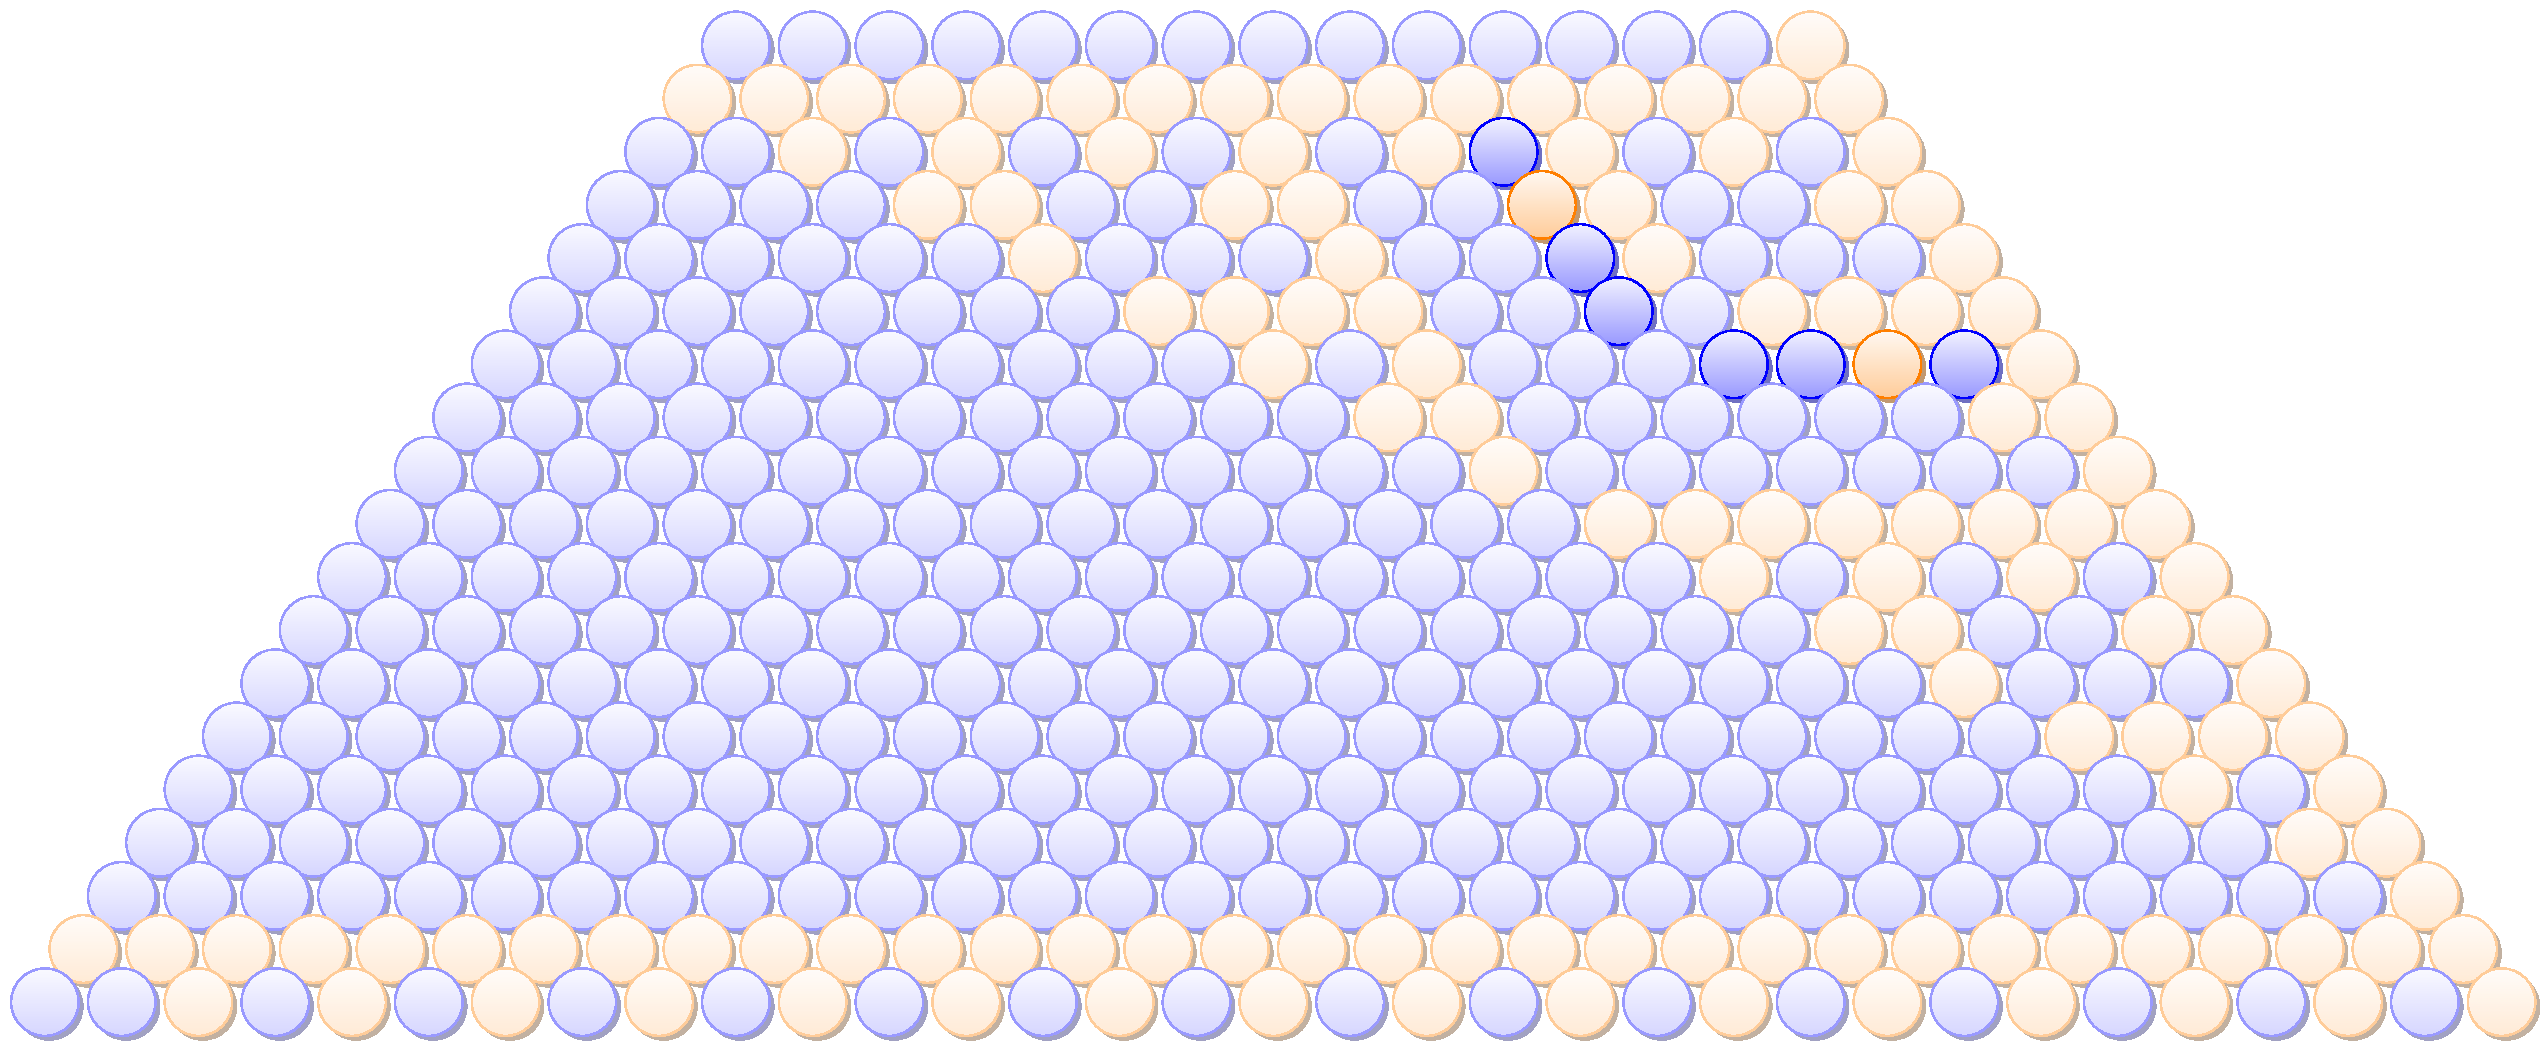
\includegraphics[width=10cm, height=10cm, keepaspectratio=true]
            {../RART2015/catalan-tikz/mirrored-clusters/mirrored-clusters.pdf}
    }

    % this 'particular' line is necessary to use `displaymath' environment
    % into the caption environment, togheter with the inclusion of 
    % `caption' package. See here for more explanation:
    % http://stackoverflow.com/questions/2716227/adding-an-equation-or-formula-to-a-figure-caption-in-latex
    \captionsetup{singlelinecheck=off}
    \caption[\emph{Mirrored} principal clusters $\mathcal{C}_{\equiv_{2}}^{(4)}$]
        {Some coefficients in \emph{mirrored} cluster $\mathcal{C}_{\equiv_{2}}^{(4)}$ 
        over $\hat{d}_{20,2^{4}-1}$: congruences $d_{20-e,2^{4}-1-e} \equiv_{2} d_{20,2^{4}-1+e}$ 
        for $e\in\lbrace1,\ldots,4\rbrace$ }

    \label{fig:catalan-mirrored-clusters}

\end{figure}

In \autoref{fig:catalan-mirrored-clusters} some coefficients in \flqq mirrored\frqq\,
cluster $\mathcal{C}_{\equiv_{2}}^{(4)}$ are highlighted.

\subsection{$\mathcal{C}_{\equiv_{2}}^{(\alpha+1)}$ 
    contains a copy of $\mathcal{C}_{\equiv_{2}}^{(\alpha)}$}

In order to fully characterize $\mathcal{C}$ in a modular context we are
left with a last theorem.

\begin{theorem}
    $\mathcal{C}_{\equiv_{2}}^{(\alpha+1)}$ 
    contains a copy of $\mathcal{C}_{\equiv_{2}}^{(\alpha)}$,
    located at the very right of its bottom half. Formally, 
    let $\Phi^{(\alpha)}=\diagup_{\lbrace 2,\ldots,2^{\alpha}-1\rbrace}^{2^{\alpha}-1}$
    be a \flqq mirror\frqq\,segment and $\hat{d}_{s,2^{{\alpha}}-1}$ 
    be a coefficient in $\Phi^{(\alpha)}$, for some $s\in rows\left(\Phi^{(\alpha)}\right)$. Then:
    \begin{displaymath}
        d_{s,2^{{\alpha}}-1+e} \equiv_{2} d_{s-2^{{\alpha}},e-1}
    \end{displaymath}
    for $e\in\lbrace1,\ldots,s-2^{{\alpha}}\rbrace$.
\end{theorem}

\begin{proof}
We tackle the proof using \autoref{eq:catalan:array:second:identity}:
\begin{displaymath}
    \hspace{-4cm}
    \begin{split}
        {{2s-(2^{{\alpha}}-1+e)}\choose{s-(2^{{\alpha}}-1+e)}} - {{2s-(2^{{\alpha}}-1+e)}\choose{s-(2^{{\alpha}}-1+e)-1}}
        &\equiv_{2}
        {{2(s-2^{{\alpha}})-(e-1)}\choose{(s-2^{{\alpha}})-(e-1)}} - {{2(s-2^{{\alpha}})-(e-1)}\choose{(s-2^{{\alpha}})-(e-1)-1}}\\
        {{2s-2^{{\alpha}}+1-e}\choose{s-2^{{\alpha}}+1-e}} - {{2s-2^{{\alpha}}+1-e}\choose{s-2^{{\alpha}}-e}}
        &\equiv_{2}
        {{2s-2^{{\alpha}+1}-e+1}\choose{s-2^{{\alpha}}-e+1}} - {{2s-2^{{\alpha}+1}-e+1}\choose{s-2^{{\alpha}}-e}}\\
        {{2s-2^{{\alpha}}+1-e}\choose{s}} - {{2s-2^{{\alpha}}+1-e}\choose{s+1}}
        &\equiv_{2}
        {{2s-2^{{\alpha}+1}-e+1}\choose{s-2^{{\alpha}}}} - {{2s-2^{{\alpha}+1}-e+1}\choose{s-2^{{\alpha}}+1}}\\
    \end{split}
\end{displaymath}
Since $e\in\lbrace1,\ldots,s-2^{{\alpha}}\rbrace$, proceed by complete induction on $e$:
    \begin{itemize}
        \item base case $e=1$ therefore:

            \begin{displaymath}
                \begin{split}
                    {{2s-2^{{\alpha}}}\choose{s}} - {{2s-2^{{\alpha}}}\choose{s+1}}
                    &\equiv_{2}
                    {{2s-2^{{\alpha}+1}}\choose{s-2^{{\alpha}}}} - {{2s-2^{{\alpha}+1}}\choose{s-2^{{\alpha}}+1}}\\
                \end{split}
            \end{displaymath}
            In the previous proof a detailed (and boring) derivation has been performed,
            here we observe that upper terms of each binomial coefficient, $2s-2^{{\alpha}}$
            and $2s-2^{{\alpha}+1}$ respectively, have $2$ in their prime factorization, therefore
            expanding each binomial, $2$ can be factored out in turn, making congruent $0$
            each one of them. However an approach similar to the previous one can be
            taken as well.

        \item assume the argument holds for $k\leq e$ and prove for $k=e+1$, so we need to show:
            \begin{displaymath}
                \hspace{-7cm}
                \begin{split}
                    {{2s-2^{{\alpha}}+1-(e+1)}\choose{s}} - {{2s-2^{{\alpha}}+1-(e+1)}\choose{s+1}}
                    &\equiv_{2}
                    {{2s-2^{{\alpha}+1}-(e+1)+1}\choose{s-2^{{\alpha}}}} - {{2s-2^{{\alpha}+1}-(e+1)+1}\choose{s-2^{{\alpha}}+1}}\\
                    {{2s-2^{{\alpha}}-e}\choose{s}} - {{2s-2^{{\alpha}}-e}\choose{s+1}}
                    &\equiv_{2}
                    {{2s-2^{{\alpha}+1}-e}\choose{s-2^{{\alpha}}}} - {{2s-2^{{\alpha}+1}-e}\choose{s-2^{{\alpha}}+1}}\\
                \end{split}
            \end{displaymath}
            which follows directly by complete induction hypothesis.
    \end{itemize}
\end{proof}


\begin{figure}[p]

    \noindent\makebox[\textwidth]{
        \centering
        %\includegraphics[width=0.8\textwidth]{../../sympy/catalan/coloured.pdf}

        % using *angle* property to rotate it is difficult to properly align it
        % in order to have a "real" matrix representation.
        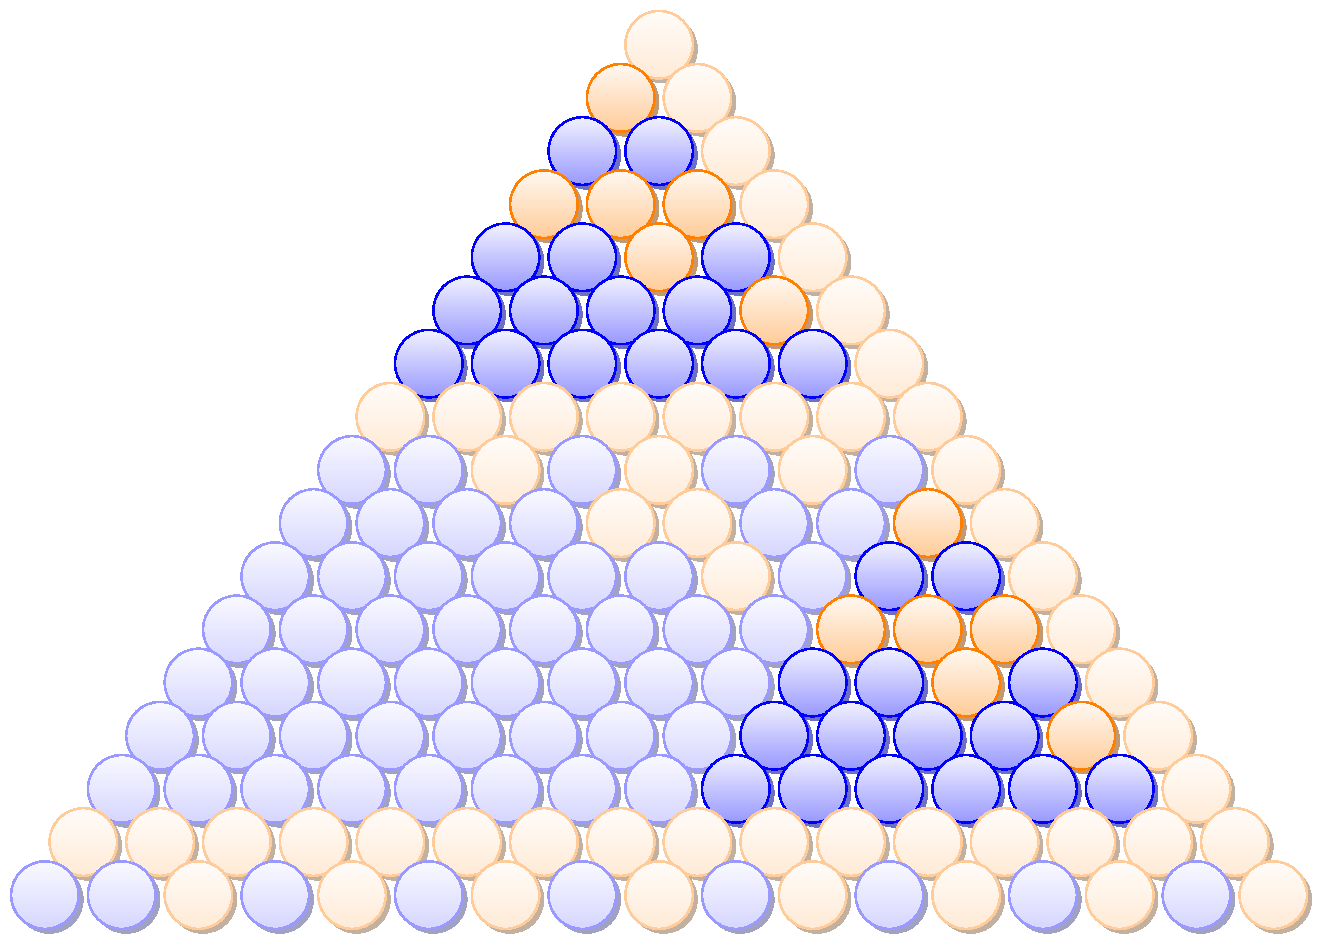
\includegraphics[width=6cm, height=6cm, keepaspectratio=true]{../RART2015/catalan-tikz/principal-cluster/principal-cluster.pdf}
    }

    % this 'particular' line is necessary to use `displaymath' environment
    % into the caption environment, togheter with the inclusion of 
    % `caption' package. See here for more explanation:
    % http://stackoverflow.com/questions/2716227/adding-an-equation-or-formula-to-a-figure-caption-in-latex
    \captionsetup{singlelinecheck=off}
    \caption[$\mathcal{C}_{\equiv_{2}}^{(4)}$ 
    contains a copy of $\mathcal{C}_{\equiv_{2}}^{(3)}$]{$\hat{d}_{s,2^{3}-1}$ for $s\in S_{2^{3}-1}$,
    $d_{s,2^{3}-1+e} \equiv_{2} d_{s-2^{3},e-1}$ with $e\in\lbrace1,\ldots,s-2^{3}\rbrace$ }

    \label{fig:catalan-principal-cluster}

\end{figure}


Before concluding the modular characterization of $\mathcal{C}$, 
we would like to observe that the last two
theorems do not say anything about the \emph{value} of remainder for 
a coefficient belonging to subtriangles of interest: 
we have only shown that a \emph{complete} subtriangle is repeated 
when coefficients are taken modulo $2$. 

\subsection{A Python prototype}

Observation in last paragraph allows us to code a bunch of Python functions, 
lying on top of SymPy module, that produce 
$\mathcal{C}_{\equiv 2}^{(\alpha+1)}$ consuming $\mathcal{C}_{\equiv 2}^{(\alpha)}$:
the construction is strictly \emph{blockwise}, according theorems stated
in previous section. Here's the implementation:

\begin{adjustwidth}{-4cm}{0cm}
    \inputminted{python}{../../PhD/projects/recurrences-unfolding/sympy-notebook/colouring.py}
\end{adjustwidth}

The following is a session that builds $\mathcal{C}_{\equiv 2}^{(7)}$:
\begin{minted}{python}
    catalan_matrix = Matrix([
        [1,0,0,0,0,0], 
        [1,1,0,0,0,0], 
        [2,2,1,0,0,0], 
        [5,5,3,1,0,0], 
        [14,14,9,4,1,0], 
        [42,42,28,14,5,1]])
    alpha = 2
    bound = 2**alpha
    pc = catalan_matrix[:bound, :bound]
    pc = pc.applyfunc(lambda c: c % 2)
    # _ = colour_matrix(pc)
    pc = build_modular_catalan(pc)
    # _ = colour_matrix(pc)
    pc = build_modular_catalan(pc)
    # _ = colour_matrix(pc)
    pc = build_modular_catalan(pc)
    # _ = colour_matrix(pc)
    pc = build_modular_catalan(pc)
    # _ = colour_matrix(pc)
    pc = build_modular_catalan(pc)
    # _ = colour_matrix(pc)
\end{minted}

Function \mintinline{python}|build_modular_catalan| implements given theorems to avoid
computing convolutions and series expansion: the starting building block in the 
above session is $\mathcal{C}_{\equiv 2}^{(2)}$, hence it is very quick. 
If desired, it is possible to display coloured triangles as svg images:
just uncomment \mintinline{python}|# _ = colour_matrix(pc)| lines.

\subsection{Some open questions}


\begin{figure}[p]

    \noindent\makebox[\textwidth]{
        \centering
        %\includegraphics[width=0.8\textwidth]{../../sympy/catalan/coloured.pdf}

        % using *angle* property to rotate it is difficult to properly align it
        % in order to have a "real" matrix representation.
        \includegraphics[width=20cm, height=20cm, keepaspectratio=true]{../sympy/catalan/catalan-traditional-inverse-ignore-negatives-centered-colouring-127-rows-mod2-partitioning-triangle.pdf}
    }

    % this 'particular' line is necessary to use `displaymath' environment
    % into the caption environment, togheter with the inclusion of 
    % `caption' package. See here for more explanation:
    % http://stackoverflow.com/questions/2716227/adding-an-equation-or-formula-to-a-figure-caption-in-latex
    \captionsetup{singlelinecheck=off}
    \caption[$\mathcal{C}_{\equiv_{2}}^{-1}$]{
        Catalan traditional triangle, formally: 
        \begin{displaymath}
            \mathcal{C}^{-1}=\left(t, t {\left(1-t\right)} \right)
        \end{displaymath} % \newline % new line no more necessary
        inverse, ignore negatives, centered colouring, 127 rows, mod2 partitioning
        }

    \label{fig:catalan-traditional-inverse-ignore-negatives-centered-colouring-127-rows-mod2-partitioning-triangle}

\end{figure}

We finish this section leaving some problems we are currently working on:
\begin{itemize}
    \item find a modular characterization of $\mathcal{C}_{\equiv_{2}}^{-1}$, reported in 
        \autoref{fig:catalan-traditional-inverse-ignore-negatives-centered-colouring-127-rows-mod2-partitioning-triangle}
    \item how the characterization described in this section can be generalized to congruences modulo an arbitrary prime $p$?
\end{itemize}


\section{Other arrays characterizations}


\cleardoublepage

\chapter{$h$-characterization}


\section{Main idea}

Consider a \emph{Riordan array} $\mathcal{R}\left(d(t),h(t)\right)$ 
defined over generating functions $d$ and $h$. 
By definition, coefficients lying on 
column $k$ are the coefficients of the following combination:
\begin{displaymath}
    d(t)h(t)^k
\end{displaymath}
our idea is to characterize $\mathcal{R}$ doing a variable change, as the
following manipulation catches:
\begin{displaymath}
    d(t)h(t)^k = d(t)(1 + (h(t)-1))^k = \left[ \left. d(\hat{h}(1+y))(1+y)^k \right|y = h(t)-1  \right]
\end{displaymath}
where function $\hat{h}$ is the compositional inverse of $h$, the one that
satisfies $\hat{h}(h(t)) = t$: in order to get $t$ back, apply $\hat{h}$ to
both members of $y+1 = h(t)$.
Inside the square brackets there's a shape of a Riordan array, therefore:
\begin{displaymath}
    \begin{split}
        \mathcal{R}\left(d(t),h(t)\right) &= \left[ \mathcal{R}\left(d(\hat{h}(1+y)), 1+y\right) \left| y = h(t)-1 \right. \right]\\
        &= \mathcal{R}_{y=h(t)-1}\left( f(y), 1+y \right) =  \mathcal{R}_{h(t)}\left( g(h(t)), h(t) \right) 
    \end{split}
\end{displaymath}
$\mathcal{R}_{y=h(t)-1}$ is interesting since its first component $f(y)$ allows to 
develop a new array $\mathcal{R}_{h(t)}$ where it's first component
is a function $g$ in the ``variable'' $h(t)$, eventually the moral is:
\begin{quote}
    \graffito{$h$-characterization}
    \emph{function composition $d$ with $\hat{h}$ yields array $\mathcal{R}_{h(t)}$,\\
        the $h$-characterization of $\mathcal{R}$, which depends on function $h$ only }
\end{quote}
It's important to understand the meaning of those new symbols:
\begin{itemize}
    \item $\mathcal{R}_{\gamma=\Omega(t)}$ denotes an array where a variable
        substitution has to take place, namely $\Omega(t)$ is the substitution 
        for variable $\gamma$;
        \marginpar{$\mathcal{R}_{t}(d(t),h(t))$ denotes verbosly, but correctly, the same
            array $\mathcal{R}(d(t),h(t))$ denotes}
    \item $\mathcal{R}_{\Omega(t)}$ denotes an array where $\Omega(t)$ should 
        be seen as a variable, like a \emph{datum}, and should not be expanded,
        even if $\Omega$'s definition is known. 
        % the same concept can be expressed as follow:
            %(a point very important to understand: here $h(t)$ shouldn't be
            %interpreted as a \emph{function}, the one in $\mathcal{R}$'s definition, instead
            %abstract over it and consider it as a \emph{variable}).
        % this has been cut from a paragraph within `Group operations, revisited' section
\end{itemize}

\label{par:h:characterization:is:an:array:polymorphism}
Moreover, the $h$-characterization $\mathcal{R}_{h(t)}\left(g(h(t)),h(t)\right)$,
\marginpar{$\mathcal{R}_{h(t)}$ is polymorphic}
for some function $g$, can be used as a Riordan array \emph{trasparently},
where traditional function $d$ satisfies $d(t) = g(h(t))$ while function $h$
is interpreted the same.


\subsection{Applying it to known triangles}

In the following sections we characterize some well known 
arrays under this development.

\subsubsection{Pascal}
Let $\mathcal{P}$ be the Riordan array for the Pascal triangle,
defined as:
\begin{displaymath} 
    \mathcal{P} = \left(\frac{1}{1-t}, \frac{t}{1-t}  \right)
\end{displaymath} 
computing the compositional inverse of $h$ yields:
\begin{displaymath} 
    \hat{h}(y) = \frac{y}{1+y}
\end{displaymath} 
so $f(y)=d(\hat{h}(1+y))=2+y$ therefore:
\begin{displaymath} 
    \mathcal{P}_{y=h(t)-1}\left( 2+y, 1+y \right)= \mathcal{P}_{h(t)}\left( 1+h(t), h(t) \right)
\end{displaymath} 
Now study the generating function which carries coefficients lying on column $k$
of $\mathcal{P}_{h(t)}$:
\marginpar{this recall the Rogers' work about \emph{renewal arrays}, 
which we described in \autoref{sec:back:to:the:basics:rogers}} 
\begin{displaymath} 
    h(t)^k + h(t)^{k+1}
\end{displaymath} 
hence column $k$ is the sum of $k$-fold and $(k+1)$-fold convolutions 
of function $h$ with itself.

\subsubsection{Fibonacci}
Let $\mathcal{F}$ be the Riordan array for the Fibonacci triangle,
defined as:
\begin{displaymath} 
    \mathcal{F} = \left(\frac{1}{1-t-t^2}, \frac{1-\sqrt{1-4t}}{2}  \right)
\end{displaymath} 
computing the compositional inverse of $h$ yields:
\begin{displaymath} 
    \hat{h}(y) = y - y^2
\end{displaymath} 
so $f(y)=d(\hat{h}(1+y))=\frac{1}{1+y-2y^3-y^4}$ therefore:
\begin{displaymath} 
    \begin{split} 
        & \mathcal{F}_{y=h(t)-1}\left( \frac{1}{1+y-2y^3-y^4}, 1+y \right) = \mathcal{F}_{h(t)}\left( \frac{1}{1-h(t)+2h(t)^3-h(t)^4}, h(t) \right)\\
    \end{split} 
\end{displaymath} 
Now study the generating function which carries coefficients lying on column $k$
of $\mathcal{F}_{h(t)}$:
\begin{displaymath} 
    \frac{h(t)^k}{1-h(t)+2h(t)^3-h(t)^4}
\end{displaymath} 

\subsubsection{Catalan}
Let $\mathcal{C}$ be the Riordan array for the Catalan triangle,
defined as:
\begin{displaymath} 
    \mathcal{C} = \left(\frac{1-\sqrt{1-4t}}{2t}, \frac{1-\sqrt{1-4t}}{2}  \right)
\end{displaymath} 
computing the compositional inverse of $h$ yields:
\begin{displaymath} 
    \hat{h}(y) = y - y^2
\end{displaymath} 
so $f(y)=d(\hat{h}(1+y))=\frac{\sqrt{4 \, y^{2} + 4 \, y + 1} - 1}{2 \, {\left(y + 1\right)} y}$ therefore:
\marginpar{$h_{\mathcal{F}}=h_{\mathcal{C}}$, here function $d$ makes the difference}
\begin{displaymath} 
    \begin{split} 
        &\mathcal{C}_{y=h(t)-1}\left(\frac{\sqrt{4 \, y^{2} + 4 \, y + 1} - 1}{2 \, {\left(y + 1\right)} y}, 1+y \right) \\
        &= \mathcal{C}_{h(t)}\left(\frac{\sqrt{4 \, h\left(t\right)^{2} - 4 \, h\left(t\right) + 1} - 1}{2 \, {\left(h\left(t\right) - 1\right)} h\left(t\right)}, h(t) \right)\\
        &= \mathcal{C}_{h(t)}\left(\frac{\sqrt{(2 h\left(t\right) -  1)^2} - 1}{2 \, {\left(h\left(t\right) - 1\right)} h\left(t\right)}, h(t) \right)\\
    \end{split} 
\end{displaymath} 
By cases on $\sqrt{(2 h\left(t\right) -  1)^2}$:
\marginpar{$\sqrt{x^{2}}=\pm x$ trick}
\begin{itemize}
    \item $\sqrt{(2 h\left(t\right) -  1)^2}=2 h\left(t\right) -  1$, hence:
        \begin{displaymath} 
            \mathcal{C}_{h(t)}\left(\frac{2(h\left(t\right) -  1)}{2 \, {\left(h\left(t\right) - 1\right)} h\left(t\right)}, h(t) \right)=
            \mathcal{C}_{h(t)}\left(\frac{1}{h\left(t\right)}, h(t) \right)
        \end{displaymath} 
        since $h(0)=0$ the previous result has no meaning, therefore discard this case;
    \item $\sqrt{(2 h\left(t\right) -  1)^2}=1 -2 h\left(t\right)$, hence:
        \begin{displaymath} 
            \mathcal{C}_{h(t)}\left(\frac{h\left(t\right)}{ {\left(1-h\left(t\right) \right)} h\left(t\right)}, h(t) \right)=
            \mathcal{C}_{h(t)}\left(\frac{1}{1-h\left(t\right)}, h(t) \right)
        \end{displaymath} 
        checking against $h(0)=0$ the previous result has meaning, therefore accept this case.
\end{itemize}
Now study the generating function which carries coefficients lying on column $k$
of $\mathcal{C}_{h(t)}$:
\begin{displaymath} 
    \frac{h(t)^{k}}{1-h\left(t\right)} 
\end{displaymath} 


\subsubsection{Motzkin, classic version}

Let $\mathcal{M}$ be the Riordan array for the Motzkin triangle, defined as:
\begin{displaymath} 
    \mathcal{M} =\left( \frac{1-t-\sqrt{1-2t-3t^2}}{2t^2}, \frac{1-t-\sqrt{1-2t-3t^2}}{2t}  \right)
\end{displaymath} 
computing the compositional inverse of $h$ yields:
\begin{displaymath} 
    \hat{h}(y) = \frac{y}{1+y+y^2}
\end{displaymath} 
so $f(y)=d(\hat{h}(1+y))$ equals:
\begin{lenghtydisplaymath} 
    \begin{split} 
        & -\frac{{\left(y^{2} \sqrt{\frac{{\left(y^{2} + 4 \, y + 4\right)} y^{2}}{{\left(y^{2} + 3 \, y + 3\right)}^{2}}} - y^{2} + 3 \, y \sqrt{\frac{{\left(y^{2} + 4 \, y + 4\right)} y^{2}}{{\left(y^{2} + 3 \, y + 3\right)}^{2}}} - 2 \, y + 3 \, \sqrt{\frac{{\left(y^{2} + 4 \, y + 4\right)} y^{2}}{{\left(y^{2} + 3 \, y + 3\right)}^{2}}} - 2\right)} {\left(y^{2} + 3 \, y + 3\right)}}{2 \, {\left(y + 1\right)}^{2}} \\
        & = -\frac{{ \left(\sqrt{\frac{{\left(y^{2} + 4 \, y + 4\right)} y^{2}}{{\left(y^{2} + 3 \, y + 3\right)}^{2}}} \left( y^{2}+3y+3 \right) -\left(y^{2}+2y+2\right)\right){\left(y^{2} + 3 \, y + 3\right)}}}{2 \, {\left(y + 1\right)}^{2}} \\
        & = -\frac{ \left(\sqrt{\left(y^{2} + 4 y + 4\right) y^{2}} -\left(y^{2}+2y+2\right)\right)\left(y^{2} + 3y + 3\right)}{2 {\left(y + 1\right)}^{2}} \\
    \end{split} 
\end{lenghtydisplaymath} 
Recognize a perfect square $y^{2} + 4 y + 4 = (y+2)^{2}$:
\marginpar{we could also stop here and reason by cases about $\pm\left(\left(y + 2\right) y\right)$
    without going on substituting variable $y$ too soon\ldots}
\begin{lenghtydisplaymath} 
        -\frac{ \left(\sqrt{\left(\left(y + 2\right) y\right)^{2}} -\left(y^{2}+2y+2\right)\right)\left(y^{2} + 3y + 3\right)}{2 {\left(y + 1\right)}^{2}} 
\end{lenghtydisplaymath} 
therefore:
\begin{lenghtydisplaymath} 
    \begin{split} 
        &\mathcal{M}_{y=h(t)-1}\left(
            -\frac{ \left(\sqrt{\left(\left(y + 2\right) y\right)^{2}} -\left(y^{2}+2y+2\right)\right)\left(y^{2} + 3y + 3\right)}{2 {\left(y + 1\right)}^{2}} , 1+y \right) \\
        &= \mathcal{M}_{h(t)}\left(
        -\frac{{\left(\sqrt{\frac{{\left(h(t)^{2} + 2 \, h(t) + 1\right)} {\left(h(t) - 1\right)}^{2}}{{\left(h(t)^{2} + h(t) + 1\right)}^{2}}}\left( h(t)^{2} + h(t) + 1\right) 
            - (h(t)^{2} + 1) \right)} {\left(h(t)^{2} + h(t) + 1\right)}}{2 \, h(t)^{2}} , h(t) \right)\\
        &= \mathcal{M}_{h(t)}\left(
        -\frac{{\left(\sqrt{\left(h(t)^2 - 1\right)^{2}} - (h(t)^{2} + 1) \right)} {\left(h(t)^{2} + h(t) + 1\right)}}{2 \, h(t)^{2}} , h(t) \right)\\
    \end{split} 
\end{lenghtydisplaymath} 
By cases on $\sqrt{\left(h(t)^2 - 1\right)^{2}}$:
\begin{itemize}
    \item $\sqrt{\left(h(t)^2 - 1\right)^{2}}= h(t)^2 - 1$, hence:
        \begin{displaymath} 
            \mathcal{M}_{h(t)}\left(\frac{ h(t)^{2} + h(t) + 1}{h(t)^{2}} , h(t) \right)\\
        \end{displaymath} 
        since $h(0)=0$ the previous result has no meaning, therefore discard this case;
    \item $\sqrt{\left(h(t)^2 - 1\right)^{2}}= 1-h(t)^2$, hence:
        \begin{displaymath} 
            \mathcal{M}_{h(t)}\left( h(t)^{2} + h(t) + 1, h(t) \right)\\
        \end{displaymath} 
        checking against $h(0)=0$ the previous result has meaning, therefore accept this case.
\end{itemize}

It is interesting to note that the tedious derivation developed above can have
a simpler handling if we defer substituting $h(t)-1$ for $y$, consider the following \ldots
by cases on $\sqrt{\left(\left(y + 2\right) y\right)^{2}}$:
\begin{itemize}
    \item $\sqrt{\left(\left(y + 2\right) y\right)^{2}}=\left(y + 2\right) y$, hence:
        \begin{displaymath} 
            \mathcal{M}_{y=h(t)-1}\left(\frac{y^{2} + 3y + 3}{{\left(y + 1\right)}^{2}} , 1+y \right) = 
                \mathcal{M}_{h(t)}\left( \frac{1+h(t)+h(t)^2}{h(t)^2}, h(t) \right) 
        \end{displaymath} 
        since $h(0)=0$ the previous result has no meaning, therefore discard this case;
    \item $\sqrt{\left(\left(y + 2\right) y\right)^{2}}=-\left(y + 2\right) y$, hence:
        \begin{displaymath} 
            \mathcal{M}_{y=h(t)-1}\left(y^{2} + 3y + 3 , h(t) \right) = 
                \mathcal{M}_{h(t)}\left( 1+h(t)+h(t)^2, h(t) \right) 
        \end{displaymath} 
        checking against $h(0)=0$ the previous result has meaning, therefore accept this case.
\end{itemize}

In both branches same definitions for $\mathcal{M}_{h(t)}$ are reached applying
same checks, while at the same time substituting variable $y$ is easier. 
\\\\
However, here it is the generating function which carries coefficients 
lying on column $k$ of $\mathcal{M}_{h(t)}$:
\begin{displaymath} 
    h(t)^{k}+h(t)^{k+1}+h(t)^{k+2}
\end{displaymath} 


\subsubsection{Motzkin, $\mathcal{T}$ variant}

Let $\mathcal{T}$ be the Riordan array for a variant
of the Motzkin array defined as:
\begin{displaymath} 
    \mathcal{T} = \left(\frac{1}{\sqrt{1-2t-3t^2}}, 
       \frac{1-t-\sqrt{1-2t-3t^2}}{2t}  \right)
\end{displaymath} 
computing the compositional inverse of $h$ yields:
\begin{displaymath} 
    \hat{h}(y) = \frac{y}{1+y+y^2}
\end{displaymath} 
so $f(y)=d(\hat{h}(1+y))=\sqrt{\left(\frac{y^2+3y+3}{(y+2)y}\right)^{2}}$ therefore:
\begin{displaymath} 
    \mathcal{T}_{y=h(t)-1}\left( \sqrt{\left(\frac{y^2+3y+3}{(y+2)y}\right)^{2}}, 1+y \right) = 
        \mathcal{T}_{h(t)}\left( \sqrt{\left(\frac{h(t)^2+h(t)+1}{h(t)^2-1}\right)^{2}}, h(t) \right) 
\end{displaymath} 
By cases on $\sqrt{\left(\frac{h(t)^2+h(t)+1}{h(t)^2-1}\right)^{2}}$:
\begin{itemize}
    \item $\sqrt{\left(\frac{h(t)^2+h(t)+1}{h(t)^2-1}\right)^{2}}=\frac{h(t)^2+h(t)+1}{h(t)^2-1}$, hence:
        \begin{displaymath} 
            \mathcal{T}_{h(t)}\left(\frac{h(t)^2+h(t)+1}{h(t)^2-1}, h(t) \right)
        \end{displaymath} 
        requirement $h(0)=0$ doesn't raise a non-sense, so use the 
        constraint $d(0)=1$, mandatory in order to have a \emph{proper} array:
        \begin{displaymath}
            \left. \frac{h(t)^2+h(t)+1}{h(t)^2-1} \right|_{t=0} = -1 \not= 1 
        \end{displaymath} 
        so discard this case;
    \item $\sqrt{\left(\frac{h(t)^2+h(t)+1}{h(t)^2-1}\right)^{2}}=\frac{h(t)^2+h(t)+1}{1-h(t)^2}$, hence:
        \begin{displaymath}
            \mathcal{T}_{h(t)}\left(\frac{h(t)^2+h(t)+1}{1-h(t)^2}, h(t) \right)
        \end{displaymath} 
        requirement $h(0)=0$ doesn't raise a non-sense, so check $d(0)=1$ again:
        \begin{displaymath}
            \left. \frac{h(t)^2+h(t)+1}{1-h(t)^2} \right|_{t=0} = 1 
        \end{displaymath} 
        which fulfill the constraint, so accept this case.
\end{itemize}
Now study the generating function which carries coefficients lying on column $k$
of $\mathcal{T}_{h(t)}$:
\marginpar{same numerator as in classic $\mathcal{M}$ array, what's
    the relation among function $d$ and multiplier $\frac{1}{1-h(t)^{2}}$?}
\begin{displaymath} 
    \frac{h(t)^{k}+h(t)^{k+1}+h(t)^{k+2}}{1-h(t)^2 }
\end{displaymath} 


\subsubsection{Delannoy}

Let $\mathcal{D}$ be the Riordan array for the Delannoy triangle, defined as:
\begin{displaymath} 
    \mathcal{D} =\left( \frac{1}{1-t}, \frac{t(1+t)}{1-t}  \right)
\end{displaymath} 
computing the compositional inverse of $h$ yields:
\begin{displaymath} 
    \hat{h}(y) = \frac{\sqrt{1+6y+y^2}-y-1}{2}
\end{displaymath} 
so $f(y)=d(\hat{h}(1+y))=\frac{2}{4 + y - \sqrt{y^2 + 8y + 8} }$ therefore:
\begin{displaymath} 
    \begin{split}
        & \mathcal{D}_{y=h(t)-1}\left( \frac{2}{4+y-\sqrt{y^2+8y+8}}, 1+y \right)\\
        &= \mathcal{D}_{h(t)}\left( \frac{2}{3+h(t)-\sqrt{h(t)^2+6h(t)+1}}, h(t) \right) \\
    \end{split}
\end{displaymath} 
Since $h(t)^2+6h(t)+1$ isn't a perfect square, no problem arises with the previous
derivation; now study the generating function which carries coefficients lying on column $k$
of $\mathcal{D}_{h(t)}$:
\begin{displaymath} 
    \frac{2\,h(t)^k}{3+h(t)-\sqrt{h(t)^2+6h(t)+1}}
\end{displaymath} 

\subsection{Points of view}

Let $\mathcal{R}\left(d(t),h(t)\right)$ be a Riordan array and $\mathcal{R}_{h(t)}$ be
its $h$-characterization.

The first point of view we would like to introduce is to see 
$\mathcal{R}_{h(t)}$ as a \emph{factorization} \marginpar{$\mathcal{R}_{h(t)}$ factorizes $\mathcal{R}$}
of $\mathcal{R}$ in terms of $h(t)$. Namely, the structure of the characterization
depends both on functions $d$ and $\hat{h}$, but the building block is function $h$
alone. Moreover, second component of $\mathcal{R}_{h(t)}$ is \emph{always} function $h$ itself,
therefore $k$-fold convolution of function $h$ with itself in the generic
$k$ column expansion is common both to $\mathcal{R}$ both to $\mathcal{R}_{h(t)}$.

The second point of view is to see $\mathcal{R}_{h(t)}$ as a \emph{schema} array 
\marginpar{$\mathcal{R}_{h(t)}$ is a schema}.
To understand this concept, abstract over $h(t)$ and think about it as a ``plugin'', 
a ``context'' that can be filled with any function $g(t)$ you like, to get a new array
$\mathcal{R}^{\stackrel{g(t)}{\rightarrow}}$ (this notation is just a reminder that the array is obtained
by plugging in $g(t)$ into the schema $\mathcal{R}_{h(t)}$). It's pretty easy, and sound, to check:
\marginpar{plugging in $h(t)$ itself within schema $\mathcal{R}_{h(t)}$ safely gets back
    to the original array $\mathcal{R}$}
\begin{displaymath}
    \mathcal{R}^{\stackrel{h(t)}{\rightarrow}} = \mathcal{R}_{y=h(t)-1}\left( d(\hat{h}(1+y)), 1+y \right) = \mathcal{R}
\end{displaymath}
while considering an arbitrary function $g(t)$:
\begin{displaymath}
    \mathcal{R}^{\stackrel{g(t)}{\rightarrow}} = \mathcal{R}_{y=g(t)-1}\left( d(\hat{h}(1+y)), 1+y \right) = 
    \left( d(\hat{h}(g(t))), g(t) \right) 
\end{displaymath}
observe how the first component of $\mathcal{R}^{\stackrel{g(t)}{\rightarrow}}$ depends on
$\mathcal{R}$ by composition of functions $d$ and $\hat{h}$. So, every array seems to have
a ``nested schema'' that allows to build new arrays.
\\\\
We finish with a theorem about arrays in the \emph{renewal} subgroup.

\begin{theorem}
    Let $\mathcal{R}\left(d(t), h(t)\right)$ be a Riordan array belonging
    to the \emph{renewal} subgroup, so $h(t)=td(t)$. Then:
    \marginpar{it can be written as $\left[\left.\mathcal{R}\left(A(y), y)\right)\right|y=h(t)\right]$
        or as $\mathcal{R}_{y=h(t)}\left(A(y), y)\right)$ too}
    \begin{displaymath}
        \mathcal{R}_{h(t)}\left(A(h(t)), h(t))\right)
    \end{displaymath}
    where $A$ is a \ac{fps} over $\mathcal{R}$'s $A$-sequence 
    $\lbrace a_i \rbrace_{i\in\mathbb{N}}$. 
\end{theorem}

\begin{proof}
    Recall that $A$-sequence of a Riordan array $\mathcal{R}\left(d(t), h(t)\right)$
    satisfies:
    \begin{displaymath}
        h(t)=tA(h(t))
    \end{displaymath}
    By hypothesis, assume $\mathcal{R}$ belongs to the \emph{renewal} subgroup, therefore
    \begin{displaymath}
        \mathcal{R}\left(A(h(t)), h(t)\right)
    \end{displaymath}
    Let $\mathcal{R}_{h(t)}\left(g(h(t)), h(t)\right)$ be the $h$-characterization of $\mathcal{R}$,
    for some function $g$. Now plug $h(t)$ into $\mathcal{R}_{h(t)}$:
    \begin{displaymath}
        \mathcal{R}^{\stackrel{h(t)}{\rightarrow}} =
            \mathcal{R}\left(g(h(t)), h(t)\right)
    \end{displaymath}
    But $\mathcal{R}^{\stackrel{h(t)}{\rightarrow}} = \mathcal{R}$, therefore 
    $[g(y)=A(y)|y=h(t)]$ follows, as required.

\end{proof}

%\marginpar{$\mathcal{R}_{h(t)}\left(A(h(t)), h(t))\right)\rightarrow
    %\mathcal{R}\left(d(t), t\,d(t)\right)$ holds too}
\marginpar{the converse is true indeed, by $A$-sequence uniqueness}
Looking at it deeply, it is possible to have a stronger formulation, namely the 
converse holds indeed: the reason for this is the unique existence of an $A$-sequence
for each Riordan array, the argument follows using $h(t)=tA(h(t))$ again .
\\\\
This little theorem shows a possible application of the factorization point of view.
Consider the Motzkin array defined as:
\begin{displaymath} 
    \mathcal{M} =\left( \frac{1-t-\sqrt{1-2t-3t^2}}{2t^2},
       \frac{1-t-\sqrt{1-2t-3t^2}}{2t}  \right)
\end{displaymath} 
Surely $\mathcal{M}$ is a renewal array and, being in the Riordan group, 
has an $A$-sequence, which satisfies $A(t)=1+t+t^2$: 
this information \emph{can't} be read from the above definition.
\\\\
\marginpar{finding $\mathcal{M}$'s $A$-sequence}
Let $h(t)=\frac{1-t-\sqrt{1-2t-3t^2}}{2t}$ be the second
component of Motzkin array $\mathcal{M}$, which factor as follows:
\begin{displaymath} 
    \mathcal{M}_{h(t)}\left( 1+h(t)+h(t)^2, h(t) \right) 
\end{displaymath} 
using this $h$-characterization, $A$-sequence $[A(y)=1+y+y^2|y=h(t)]$ can
be read from $\mathcal{M}_{h(t)}$'s first component directly, without
solving the equation as usual:
\begin{displaymath} 
    \frac{1-t-\sqrt{1-2t-3t^2}}{2t} = t\,A\left(\frac{1-t-\sqrt{1-2t-3t^2}}{2t}\right)
\end{displaymath} 




\section{Group operations, revisited}

In this section we revise \emph{Riordan group} concepts described in
\autoref{subsection:back:to:the:basics:riordan:group}, looking at them under
the light of $h$-characterization. In particular, we show how a Riordan arrays
written using the proposed characterization, allows us to build new arrays
respect to group operation $\cdot$ and to find their inverses.

\subsection{Inverting an array}

Let $\mathcal{R}\left(d(t),h(t)\right)$ be a Riordan array and let 
$\mathcal{R}_{h(t)}\left(g(h(t)),h(t)\right)$ its $h$-characterization, for some
function $g$. %in the variable $h(t)$. 
 
Using rules for inversion in the Riordan group, 
\marginpar{using $\mathcal{R}_{h(t)}$ 
polymorphically as an array, remind \autoref{par:h:characterization:is:an:array:polymorphism}}
proceed as follow:
\begin{displaymath}
    \mathcal{R}_{h(t)}^{-1}\left(\frac{1}{g(h(\hat{h}(t)))},\hat{h}(t)\right)=
    \left[\mathcal{R}^{-1}\left(\left.\frac{1}{g(h(y))},y\right) \right| y = \hat{h}(t) \right]=
    \mathcal{R}_{\hat{h}(t)}^{-1}\left(k(\hat{h}(t)),\hat{h}(t)\right)
\end{displaymath}
where function $k$ is defined as $k(y)=\frac{1}{g(h(y))}$, 
therefore we got a new array $\mathcal{T}_{\hat{h}(t)}$ which is the $\hat{h}$-characterization
of $\mathcal{R}_{h(t)}^{-1}$ and, as the same time, of $\mathcal{R}^{-1}$.
\marginpar{again, $\hat{h}(t)$ plays the role of a \emph{variable},
so don't be tempted to say $h(\hat{h}(t))=t$ as in the normal course of things \ldots}
\\\\
For the sake of clarity we apply the previous derivation to build the inverse of $\mathcal{F}$,
the Fibonacci array.  To set the stage we need function $h$, take it from the definition:
\begin{displaymath}
    \begin{split}
        h(t)&=\frac{1-\sqrt{1-4t}}{2}\\
    \end{split}
\end{displaymath}
we need also function $g$, take it from the $h$-characterization $\mathcal{F}_{h(t)}$:
\begin{displaymath}
    \left[g(y)=\left.\frac{1}{1-y+2y^3-y^4} \right| y=h(t)\right]
\end{displaymath}
we're ready to apply:
\begin{displaymath}
    \left[\mathcal{F}^{-1}\left.\left(1-y-y^2,y\right) \right| y = \hat{h}(t) \right]=
    \mathcal{F}_{\hat{h}(t)}^{-1}\left(1-\hat{h}(t)-\hat{h}(t)^2,\hat{h}(t)\right)
\end{displaymath}
where function $\hat{h}$ is the compositional inverse of function $h$. Observe
that $1-y-y^2$ in the left array under variable constraint $y=\hat{h}(t)$, is
obtained by evaluating $\frac{1}{g(h(y))}$, considering $y$ as a variable:
using this abstraction, function $\hat{h}(t)$ cannot be used
\emph{functionally}, otherwise $g(h(\hat{h}(k)))=g(k)$, where $k=h(t)$
according to constraint under $g$ is defined. If that would be the case, it
yields a factorization in $h(t)$, not in $\hat{h}(t)$, as we would like to
have.

If the explicit definition for $\mathcal{F}^{-1}$ is desired, just plug $\hat{h}(t)=t-t^2$:
\begin{displaymath}
    \left(\mathcal{F}_{\hat{h}(t)}^{-1}\right)^{\stackrel{\hat{h}(t)}{\rightarrow}} =
        \mathcal{F}^{-1}\left(1-t+2t^3-t^4,t-t^2\right)
\end{displaymath}

\subsection{Multiplying two arrays}

Finally, let us tackle the product of two Riordan arrays. 
Multiplication, the action of the Riordan group, between two elements 
$\mathcal{A}(d_{\mathcal{A}}(t), h_{\mathcal{A}}(t))$ and 
$\mathcal{B}(d_{\mathcal{B}}(t), h_{\mathcal{B}}(t))$ belonging to the group, is defined as:
\begin{displaymath}
    \mathcal{A}\mathcal{B} = \left(d_{\mathcal{A}}(t)d_{\mathcal{B}}(h_{\mathcal{A}}(t)),
        h_{\mathcal{B}}(h_{\mathcal{A}}(t))\right)
\end{displaymath}
Consider the $h_{\mathcal{A}}$-characterization of $\mathcal{A}$:
\begin{displaymath}
    \mathcal{A}_{h_\mathcal{A}(t)} \left(\gamma(h_{\mathcal{A}}(t)), h_{\mathcal{A}}(t)  \right)
\end{displaymath}
for some function $\gamma$, and the $h_{\mathcal{B}}$-characterization of $\mathcal{B}$:
\begin{displaymath}
    \mathcal{B}_{h_\mathcal{B}(t)} \left(\eta(h_{\mathcal{B}}(t)), h_{\mathcal{B}}(t)  \right)
\end{displaymath}
for some function $\eta$, respectively. Apply now the multiplication rule:
\begin{displaymath}
    \begin{split}
        & \left(\gamma(h_{\mathcal{A}}(t)), h_{\mathcal{A}}(t)  \right)
            \left(\eta(h_{\mathcal{B}}(t)), h_{\mathcal{B}}(t)  \right) \\
        &=\left[\left.\left(\gamma(y), y  \right)
            \left(\eta(h_{\mathcal{B}}(t)), h_{\mathcal{B}}(t)  \right) \right| y=h_{\mathcal{A}}(t) \right]\\
        &=\left[\left.\left(\gamma(y)\eta(h_{\mathcal{B}}(y)), h_{\mathcal{B}}(y)  \right) \right|
             y=h_{\mathcal{A}}(t) \right]\\
    \end{split}
\end{displaymath}
Stop here, it's enough to build the $h_{\mathcal{A}}$-characterization 
of the product $\mathcal{A}\mathcal{B}$:
\begin{displaymath}
        \left[\left.\left(\Omega(y), h_{\mathcal{B}}(y)  \right) \right| y=h_{\mathcal{A}}(t) \right] 
        =\big(\mathcal{A}\mathcal{B}\big)_{h_{\mathcal{A}}(t)}\left(
            \Omega(h_{\mathcal{A}}(t)), h_{\mathcal{B}}(h_{\mathcal{A}}(t))  \right)
\end{displaymath}
where $\left[\left.\Omega(y)= \gamma(y)\eta(h_{\mathcal{B}}(y))\right| y=h_{\mathcal{A}}(t) \right]$. 
\\\\
Nonetheless, 
\marginpar{The following can be skipped on a first reading}
from were we stopped, it's possible to factor $\mathcal{A}\mathcal{B}$ respect to $h_{\mathcal{B}}(t)$ in
a similar way, this time abstracting over $h_{\mathcal{B}}(y)$, remembering to track $y=h_{\mathcal{A}}(t)$:
\begin{displaymath}
    \begin{split}
        &\left[\left.\left(\gamma(y)\eta(h_{\mathcal{B}}(y)), h_{\mathcal{B}}(y)  \right) \right|
             y=h_{\mathcal{A}}(t) \right]\\
        &=\left.\left[\left.\left(\gamma(\hat{h}_{\mathcal{B}}(k))\eta(k), k  \right) \right|
             k=h_{\mathcal{B}}(y) \right]\right|_{y=h_{\mathcal{A}}(t)}\\
        &=\left.\left[\left.\left(\Theta(k), k  \right) \right| k=h_{\mathcal{B}}(y) \right]\right|_{y=h_{\mathcal{A}}(t)}\\
        &=\left.\big(\mathcal{A}\mathcal{B}\big)_{h_{\mathcal{B}}(y)}\left(
            \Theta(h_{\mathcal{B}}(y)), h_{\mathcal{B}}(y)  \right)\right|_{y=h_{\mathcal{A}}(t)}
    \end{split}
\end{displaymath}
\marginpar{in order to stop tracking $y=h_{\mathcal{A}}(t)$, we should write $(\Theta(k), k)$,
    where $k$ solves
    $h_{\mathcal{B}}(\hat{h}_{\mathcal{A}}(\hat{h}_{\mathcal{B}}(k)))=h_{\mathcal{B}}(t)$,
    but it doesn't supply an explicit variable substitution}
where $\left.\left[\left.\Theta(k)=\gamma(\hat{h}_{\mathcal{B}}(k))\eta(k) \right| 
    k=h_{\mathcal{B}}(y) \right]\right|_{y=h_{\mathcal{A}}(t)}$.

Observe that for the latter factorization, it is necessary to compute function $\hat{h}_{\mathcal{B}}$, 
the compositional inverse of function $h_{\mathcal{B}}$.
\\\\
For the sake of clarity we apply the previous derivation to the product $\mathcal{P}\mathcal{F}$, namely
we'll multiply Pascal and Fibonacci arrays, \emph{in the given order}, providing 
both $\big(\mathcal{P}\mathcal{F}\big)_{h_{\mathcal{P}}(t)}$ 
and $\left.\big(\mathcal{P}\mathcal{F}\big)_{h_{\mathcal{F}}(y)}\right|_{y=h_{\mathcal{P}}(t)}$.

Recall $\mathcal{P}$ and $\mathcal{F}$ $h$-characterizations, they are respectively:
\begin{displaymath}
    \begin{split}
        &\mathcal{P}_{h_{\mathcal{P}}(t)}\left( 1+h_{\mathcal{P}}(t), h_{\mathcal{P}}(t) \right)
            \text{ where } h_{\mathcal{P}}(t) = \frac{t}{1-t}\\
        &\mathcal{F}_{h_{\mathcal{F}}(t)}\left( \frac{1}{1-h_{\mathcal{F}}(t)+
            2h_{\mathcal{F}}(t)^3-h_{\mathcal{F}}(t)^4}, h_{\mathcal{F}}(t) \right)
                \text{ where } h_{\mathcal{F}}(t) = \frac{1-\sqrt{1-4t}}{2}\\
    \end{split}
\end{displaymath}
and recognize the following functions under variable constraint (in the following, $y$
is a ``local'' variable, \emph{it's not shared} among the two definitions):
\begin{displaymath}
    \begin{split}
        &\left.\left[\gamma(y) = 1+y \right| y=h_{\mathcal{P}}(t) \right]\\
        &\left.\left[\eta(y) = \frac{1}{1-y+2y^3-y^4} \right| y=h_{\mathcal{F}}(t) \right]\\
    \end{split}
\end{displaymath}

Toward $\big(\mathcal{P}\mathcal{F}\big)_{h_{\mathcal{P}}(t)}$, compute $\Omega$ function:
\begin{displaymath}
    \left.\left[\Omega(y)= \gamma(y)\eta(h_{\mathcal{F}}(y))\right| y=h_{\mathcal{P}}(t) \right]
        = \left.\left[\Omega(y)= \frac{1+y}{1-y-y^2}\right| y=h_{\mathcal{P}}(t) \right]
\end{displaymath}
\marginpar{$\big(\mathcal{P}\mathcal{F}\big)_{h_{\mathcal{P}}(t)}$}
therefore answer the first question:
\begin{displaymath}
    \big(\mathcal{P}\mathcal{F}\big)_{h_{\mathcal{P}}(t)} \left(\frac{1+
        h_{\mathcal{P}}(t)}{1-h_{\mathcal{P}}(t)-h_{\mathcal{P}}(t)^2}, \frac{1-\sqrt{1-4h_{\mathcal{P}}(t)}}{2} \right)
\end{displaymath}

\marginpar{$\left.\big(\mathcal{P}\mathcal{F}\big)_{h_{\mathcal{F}}(y)}\right|_{y=h_{\mathcal{P}}(t)}$}
Toward $\left.\big(\mathcal{P}\mathcal{F}\big)_{h_{\mathcal{F}}(y)}\right|_{y=h_{\mathcal{P}}(t)}$, compute $\Theta$ function:

\begin{displaymath}
    \begin{split}
        &\left.\left[\left.\Theta(k)=\gamma(\hat{h}_{\mathcal{F}}(k))\eta(k) \right| k=h_{\mathcal{F}}(y) \right]\right|_{y=h_{\mathcal{P}}(t)}\\
        &= \left.\left[\left.\Theta(k)=\frac{1+k-k^2}{1-k+ 2k^3 - k^4} \right| k=h_{\mathcal{F}}(y) \right]\right|_{y=h_{\mathcal{P}}(t)}\\
    \end{split}
\end{displaymath}
where $\hat{h}_{\mathcal{F}}(y)=y-y^2$, therefore answer the second question:
\begin{displaymath}
    \left.\big(\mathcal{P}\mathcal{F}\big)_{h_{\mathcal{F}}(y)} \left(
        \frac{1+h_{\mathcal{F}}(y)-h_{\mathcal{F}}(y)^2}{1-h_{\mathcal{F}}(y)+ 2h_{\mathcal{F}}(y)^3 - h_{\mathcal{F}}(y)^4} ,
        h_{\mathcal{F}}(y) \right)\right|_{y=h_{\mathcal{P}}(t)}
\end{displaymath}

\marginpar{check substituting functions $h_{\mathcal{P}}$ and $h_{\mathcal{F}}$}
Little check plugging in function $h_{\mathcal{P}}(t)$:
\begin{displaymath}
    \left(\big(\mathcal{P}\mathcal{F}\big)_{h_{\mathcal{P}}(t)}\right)^{\stackrel{h_{\mathcal{P}}(t)}{\rightarrow}}
        = \big(\mathcal{P}\mathcal{F}\big)\left(\frac{1-t}{1-3t+t^2}, \frac{1}{2}-\frac{1}{2}\sqrt{\frac{1-5t}{1-t}} \right)
\end{displaymath}
on the other hand, plugging in function $h_{\mathcal{F}}(y)$, where $y=h_{\mathcal{P}}(t)$:
\begin{displaymath}
    \left.\left(\big(\mathcal{P}\mathcal{F}\big)_{h_{\mathcal{F}}(y)}\right)^{\stackrel{h_{\mathcal{F}}(y)}{\rightarrow}}\right|_{y=h_{\mathcal{P}}(t)}
        = \left.\big(\mathcal{P}\mathcal{F}\big)\left(\frac{1+y}{1-y-y^2}, \frac{1-\sqrt{1-4y}}{2} \right)\right|_{y=h_{\mathcal{P}}(t)}
\end{displaymath}



\section{Sequences, sequences and sequences}

Every Riordan array $\mathcal{R}$, as we've seen in 
\autoref{sec:back:to:the:basics:sequences}, has a particular sequence 
$\lbrace a_i\rbrace_{i\in\mathbb{N}}$,
called $A$-sequence, such that uniquely characterizes it (to be precise another sequence
$\lbrace z_i\rbrace_{i\in\mathbb{N}}$, called $Z$-sequence, is needed 
to fulfill the very first column, together with root element $d_{00}$), 
capturing the way every element $d_{n+1,k+1}$ can be written as a linear combination
of elements lying on the previous row, formally:
\begin{displaymath}
    d_{n+1,k+1} = a_{0}d_{n,k} +a_{1}d_{n,k+1} +a_{2}d_{n,k+2} + 
        \ldots + a_{j}d_{n,k+j}
\end{displaymath}
where $k+j = n$. In this section we would like to offer a generalization
of this \emph{combinatorial device}, providing a machinery to build sequences 
that combine coefficients, possibly lying on arbitrary rows, as desired.
Finally, a connection with $A$-matrix concept is explored, leaving an open 
question.

What follows doesn't use the $h$-characterization concept directly, 
we put it here because a \emph{column oriented}
approach, as used for derivation of $h$-characterizations, is used as well. 
For the sake of simplicity,
however, we start from an array $\mathcal{R}(d(t),h(t))$ and its 
$h$-characterization $\mathcal{R}_{h(t)}(g(h(t)), h(t))$, for some function $g$.

\subsection{Localizing $A$-sequences}

Consider the following question: there exists a sequence 
$\lbrace \gamma_{i} \rbrace_{i\in\mathbb{N}}$ of coefficients 
such that the generic element $d_{n+1,k+1}\in\mathcal{R}$ can be written
as a linear combination of \emph{all} other elements $d_{n,j}$ 
lying on the previous row, namely for all $j\in\lbrace0,1,2,\ldots,n\rbrace$? 
Later we ask a more general question, for now tackle the current one.

The previous statement can be written in a compact way, or \emph{column-wise}, as:
\begin{displaymath}
    g(h(t))h(t)^k = \sum_{i\geq0}{\gamma_i\,t\,g(h(t)) h(t)^i}\\
\end{displaymath}
To see why, recall a generic column 
$k$ has generating function $g(h(t))h(t)^k$ and imagine that series written vertically, 
with increasing degree of $t$ from top to bottom.
The required constraint on coefficient of $t^n$, namely $d_{nk}$, 
to be a linear combination of elements lying on the previous row 
can be satisfied if we \emph{shift downward} every column,
namely multiplying each one by $t$, and combining them using coefficients
$\lbrace \gamma_{i} \rbrace_{i\in\mathbb{N}}$. 
We have learnt this trick from \citeauthor{shapiro:1991}, in \cite{shapiro:1991}.

Simplification of $g(h(t))$ shows that using the factored representation or
the natural one doesn't make any difference, therefore:
\begin{displaymath}
    h(t)^k = t \sum_{i\geq 0}{\gamma_i\,h(t)^i} = t \Gamma(h(t))
\end{displaymath}
where function $\Gamma$ is a \ac{fps} over sequence 
$\lbrace \gamma_{i} \rbrace_{i\in\mathbb{N}}$, which we're searching for.
Doing a change of variable to abstract over $h(t)$, its possible to
\marginpar{$\hat{h}(y)^{\alpha}$ acts as a ruler which,
    if an element $d_{nk}$ is combined,
    scrolls to row $n-\alpha$}
structure the basic for a generic schema (or \emph{device} if you please):
\begin{displaymath}
    \left.\left[y^{k} = \hat{h}(y)\,\Gamma(y) \right| y = h(t) \right]
\end{displaymath}

Before going on, let the device consumes some known arrays. Take 
array $\mathcal{C}$, so $\hat{h}_{\mathcal{C}}(y) = y-y^2$, hence:
\begin{displaymath}
    \left.\left[\frac{y^{k-1}}{1-y} =  \Gamma(y) \right| y = h(t) \right]\\
\end{displaymath}
so sequence $\lbrace \gamma_{i} \rbrace_{i\in\mathbb{N}}$ satisfies:
\begin{displaymath}
    \lbrace \gamma_{i} \rbrace_{i\in\mathbb{N}} = 
        \left(\underbrace{\gamma_{0}=0,\ldots,\gamma_{k-2}=0}_{k-1 \text{ zeros}},
            \underbrace{\gamma_{k-1}=1, \ldots}_{\text{infinitely many ones}} \right)
\end{displaymath}
so $d_{nk}\in\mathcal{C}$ is the combination of \emph{all} coefficients
lying on previous row $n-1$ according $\lbrace \gamma_{i} \rbrace_{i\in\mathbb{N}}$,
therefore $d_{nk}=\sum_{i=k-1}^{n-1}{d_{n-1,i}}$.
\marginpar{exactly as $A_{\mathcal{C}}(t)=\frac{1}{1-t}$ requires} 

Motzkin's turn, 
$\hat{h}_{\mathcal{M}}(y) = \frac{y}{1+y+y^2}$, hence:
\begin{displaymath}
        \left.\left[y^{k-1}+y^{k}+y^{k+1}=\Gamma(y)\right| y = h(t) \right]
\end{displaymath}
so sequence $\lbrace \gamma_{i} \rbrace_{i\in\mathbb{N}}$ satisfies:
\begin{displaymath}
    \lbrace \gamma_{i} \rbrace_{i\in\mathbb{N}} = 
        \left(\underbrace{\gamma_{0}=0,\ldots,\gamma_{k-2}=0}_{k-1 \text{ zeros}},
            1,1,1,
            \underbrace{\gamma_{k+2}=0, \ldots}_{\text{infinitely many zeros}} \right)
\end{displaymath}
\marginpar{exactly as $A_{\mathcal{M}}(t)=1+t+t^{2}$ requires} 
so $d_{nk}\in\mathcal{M}$ is the combination of \emph{all} coefficients
lying on previous row $n-1$ according $\lbrace \gamma_{i} \rbrace_{i\in\mathbb{N}}$,
therefore $d_{nk}=d_{n-1,k-1}+d_{n-1,k}+d_{n-1,k+1}$.
\\\\
\marginpar{getting $A$-sequence back}
What we've done is nothing more nothing less than writing $A$-sequences 
in a more generic format, putting evidence on the \emph{local} meaning 
of the combination: it is explicitly written the dependency of 
elements belonging to a column $k$. On the other hand, natural $A$-sequences 
are stated with a fixed start index in mind, namely $k-1$ if combining 
for elements in a column $k$.

\marginpar{$y^{\beta}$ acts as a second ruler too, which scrolls
    to column $\beta$ directly. Rulers $y^{k-1}$ and $\hat{h}(y)$ 
    scroll to column $k-1$ and to row $n-1$ respectively, after 
    combination starts as $\Gamma$ says\ldots}
It is possible to get the natural $A$-sequence back by requiring that 
combination of elements (denoted by coefficients of \ac{fps} $\Gamma$)  
lying on the previous row (denoted by $\hat{h}(y)$)
starts at index $k-1$ (denoted by $y^{k-1}$), formally:
\begin{displaymath}
    \left[y^{k} = y^{k-1}\,\hat{h}(y)\,\Gamma(y) \big| y = h(t) \right] = 
    \left[y = \hat{h}(y)\,\Gamma(y) \big| y = h(t) \right]
\end{displaymath}
since $h(t) = t\,A(h(t))$, then \ac{fps}
$\Gamma$ and $A$ are defined over the same sequence, the $A$-sequence, as desired.
\\\\
\marginpar{The following can be skipped on a first reading}
Here there are a couple of applications. 

What if we ask: find a sequence $\lbrace \gamma_{i} \rbrace_{i\in\mathbb{N}}$ 
such that an element $d_{nk}\in\mathcal{C}$ combines elements lying on a
row $3$ lines above, starting from column index $2$, 
namely $d_{n-3,k}$ for all $k\in\lbrace 2,\ldots,n-3\rbrace$. 
Set the device:
\begin{displaymath}
    \left[y^{k} = y^{2}\,\hat{h}(y)^3\,\Gamma(y) \big| y = h(t) \right] =
        \left.\left[\frac{y^{k-5}}{(1-y)^3} = \Gamma(y) \right| y = h(t) \right]
\end{displaymath}

Checking what we've obtained, assume you want to find coefficient $d_{7,5}$, 
chosen at random, so expand function $\Gamma$ with $k=5$:
\begin{displaymath}
    \left.\left[\Gamma(y)=1 + 3y + 6y^2 + 10y^3 + 15y^4 + \mathcal{O}(y^5) 
        \big| y = h(t) \right]\right|_{k=5}
\end{displaymath}
therefore $d_{7,5}=d_{4,2} + 3\,d_{4,3} + 6\,d_{4,4}$, 
instantiating $27 = 9 + 3\cdot4 + 6\cdot1$, which holds.
Just another element, say $d_{9,7}$, so expand function $\Gamma$ with $k=7$:
\marginpar{varing $k$ shifts $\lbrace \gamma_{i}\rbrace_{i\in\mathbb{N}}$ only.
    In \autoref{par:generalized:A:sequence:Delannoy:example}
    we will get a new sequence for each $k$}
\begin{displaymath}
    \left.\left[\Gamma(y)=y^2 + 3y^3 + 6y^4 + 10y^5 +  \mathcal{O}(y^6) 
        \big| y = h(t) \right]\right|_{k=7}
\end{displaymath}
therefore $d_{9,7}=d_{6,4} + 3\,d_{6,5} + 6\,d_{6,6}$, 
instantiating $44 = 20 + 3\cdot6 + 6\cdot1$, which holds.
It's interesting to observe the following fact: while a natural $A$-sequence
says how to combine starting always from the previous column index; with
this generalization we got the same coefficients for combining as $A$-sequence
states, augmenting with the column index from where the combination should start.

The previous two checks shows exactly this aspect: for column index $k=5$
combination starts at column index $2$, while for column index $k=7$ combination
starts at column index $4$.
\\\\
One last application, before the interlude: 
find a sequence $\lbrace \gamma_{i} \rbrace_{i\in\mathbb{N}}$ such that 
an element $d_{nk}\in\mathcal{M}$ combines \emph{all} elements lying on 
the next row, namely $d_{n+1,k}$ for all $k\in\lbrace0,\ldots,n+1\rbrace$.
The first step is always setting the device:
\begin{displaymath}
    \left[y^{k} = \hat{h}(y)^{-1}\,\Gamma(y) \big| y = h(t) \right]=
        \left[ \frac{y^{k + 1}}{y^2 + y + 1} = \Gamma(y) \big| y = h(t) \right]
\end{displaymath}
in order to find $d_{6,3}$, chosen at random, expand function $\Gamma$ with $k=3$:
\begin{displaymath}
    \left.\left[\Gamma(y)=y^4 -y^5 + y^7 -y^8 +y^{10} + \mathcal{O}(y^{11}) 
        \big| y = h(t) \right]\right|_{k=3}
\end{displaymath}
therefore $d_{6,3}=d_{7,4} - d_{7,5} + d_{7,7}$, instantiating $44 = 70 -27 +1$, 
which holds. Just another element, say $d_{8,1}$, so expand function 
$\Gamma$ with $k=1$:
\begin{displaymath}
    \left.\left[\Gamma(y)=y^2 -y^3 + y^5 -y^6 + y^8 -y^9 + y^{11} + 
        \mathcal{O}(y^{12}) \big| y = h(t) \right]\right|_{k=1}
\end{displaymath}

\marginpar{what about $d_{n0}\in\mathcal{M}$? 
    it should provide a combinatorial identity for the $n$th
    Motzkin number\ldots}
therefore $d_{8,1}=d_{9,2} - d_{9,3} + d_{9,5}- d_{9,6}+ d_{9,8}- d_{9,9}$, 
instantiating $512 = 1422 -1140 +369 -147 +9 -1$, which holds.
\\\\
As a final remark, under the insights of two solved exercises, is that a
sequence found using this approach, knows which elements to combine and which
ones to discard, we're required to supply the set of available elements only.


\subsection{Interlude: let's generalize}
\label{subsec:sequences:interluce:generalization}

Previous applications shows a pattern that can be pointed out looking at 
the generic device for a Riordan array $\mathcal{R}$ where 
function $h$ is its second component and function $\hat{h}$ 
is its compositional inverse:
\begin{displaymath}
    \left[y^{k} = \hat{h}(y) \Gamma(y) \big| y = h(t) \right]
\end{displaymath}
there's \emph{an equation} on the left hand side of the variable substitution block, 
where function $\Gamma$ is the unknown. In this format, 
a constraint is stated: let $d_{nk}\in\mathcal{R}$ be a generic element, 
then a \emph{localized} sequence 
$\lbrace \gamma_{i} \rbrace_{i\in\mathbb{N}}$ respect column $k$ exists, which
combines all elements lying on the previous row $n-1$.

Since we're dealing with an equation, we can augment it as desired in order to
constrain over additional facts. For instance, consider the following question:
find a sequence $\lbrace \gamma_{i} \rbrace_{i\in\mathbb{N}}$ such that 
an element $d_{nk}\in\mathcal{R}$ combines \emph{all} elements lying on 
\emph{some} row $n-\alpha$, with the additional property to add the combination of 
elements, defined by a \emph{given} sequence $\lbrace \theta_{i} \rbrace_{i\in\mathbb{N}}$, 
lying on \emph{some different} row $n-\beta$. Formally, $\alpha,\beta\in\mathbb{Z}$ 
and $\alpha \not=\beta$, we would like to express $d_{nk}$ as:
\begin{displaymath}
    d_{nk} = \sum_{i=0}^{n-\alpha}{\gamma_{i}\,d_{n-\alpha,i}} + 
        \sum_{i=0}^{n-\beta}{\theta_{i}\,d_{n-\beta,i}}
\end{displaymath}
so set the device as usual:
\begin{displaymath}
    \left[y^{k} = \hat{h}(y)^{\alpha} \Gamma(y) + \hat{h}(y)^{\beta} \Theta(y) \big| y = h(t) \right]
\end{displaymath}
Nonetheless its generality, its not the best one: to be truly general,
we should introduce two new parameters $c_\mu$ and $c_\nu$, which allow
to fix the column index from where the combinations denoted by functions
$\Gamma$ and $\Theta$ start, respectively. Here is the most general device:
\marginpar{most general device}
\begin{displaymath}
    \left[y^{k} = y^{c_\mu}\hat{h}(y)^{\alpha} \Gamma(y) + 
        y^{c_\nu}\hat{h}(y)^{\beta} \Theta(y) \big| y = h(t) \right]
\end{displaymath}
\\\\
\paragraph{An example about $\mathcal{D}$}{
    \label{par:generalized:A:sequence:Delannoy:example}
    \marginpar{an example about $\mathcal{D}$}
    Try to make the generalization at work:
    find a sequence $\lbrace \gamma_{i} \rbrace_{i\in\mathbb{N}}$ such that 
    an element $d_{nk}\in\mathcal{D}$, in the Delannoy array, 
    combines \emph{all} elements lying on 
    the next row, namely $n+1$, in addition to the
    combination of elements lying two row above, namely $n-2$, 
    defined as their sum, simply. 

    In order to set the device, we need $\hat{h}_{\mathcal{D}}$:
    \begin{displaymath} 
        \hat{h}_{\mathcal{D}}(y) = \frac{\sqrt{1+6y+y^2}-y-1}{2}
    \end{displaymath} 
    and build function $\Theta$ from the additional requirement:
    \begin{displaymath} 
        \Theta(y) = \frac{1}{1-y}
    \end{displaymath} 
    now we're ready:
    \begin{lenghtydisplaymath}
    \begin{split}
        &\left.\left[y^{k} = \hat{h}_{\mathcal{D}}(y)^{-1} \Gamma(y) + 
            \hat{h}_{\mathcal{D}}(y)^{2}\frac{1}{1-y} \right| y = h(t) \right]\\
        &=\left.\left[\frac{y^{3} + {\left(y^{2} - 1\right)} y^{k} + 6 \, y^{2} - {\left({\left(y - 1\right)} y^{k} + y^{2} + 3 \, y + 1\right)} \sqrt{y^{2} + 6 \, y + 1} + 6 \, y + 1}{2 \, {\left(1-y\right)}}=\Gamma(y) \right| y = h(t) \right]\\
    \end{split}
    \end{lenghtydisplaymath}
    in order to find $d_{8,1}$, chosen at random, expand function $\Gamma$ with $k=1$:
    \begin{lenghtydisplaymath}
        \left.\left[\Gamma(y)=y^2 -3y^3 + 11y^4  -47y^5 + 211y^6 -987y^7 + 4747y^8 
            -23335y^9 + \mathcal{O}(y^{10}) \big| y = h(t) \right]\right|_{k=1}
    \end{lenghtydisplaymath}
    therefore $d_{8,1}=d_{9,2} -3\,d_{9,3} +11\,d_{9,4}-47\,d_{9,5} 
        +211\,d_{9,6} -987\,d_{9,7} +4747\,d_{9,8}-23335\,d_{9,9}+\epsilon$,
        where $\epsilon = d_{6,0}+d_{6,1}+d_{6,2}+d_{6,3}+d_{6,4}+d_{6,5}+d_{6,6} = 
                2(d_{6,0}+d_{6,1}+d_{6,2})+d_{6,3} = 2(1 + 11 + 41) + 63 = 169$: 
        instantiating $15 = 113 -3\cdot377 +11\cdot681 -47\cdot681 +211\cdot377
            -987\cdot113 +4747\cdot17 -23335 + \epsilon = -154 + 169$, which holds.

    It's interesting to observe that function $\Gamma$ above, an algebraic one,
    produces sequences that use different coefficients for different values of $k$,
    and we observe a curious pattern for increasing values of 
    $k\in\lbrace 0,\ldots,10 \rbrace$:
    \begin{lenghtydisplaymath}
        \begin{split}
            &\left.\left[\Gamma(y)=
            1 y + {(-2)} y^{2} + 5 y^{3} + {(-17)} y^{4} + 65 y^{5} + {(-273)} y^{6} + 1213 y^{7} + {(-5617)} y^{8} + \mathcal{O}\left(y^{9}\right)
                \big| y = h(t) \right]\right|_{k=0}\\
            &\left.\left[\Gamma(y)=
            1 y^{2} + {(-3)} y^{3} + 11 y^{4} + {(-47)} y^{5} + 211 y^{6} + {(-987)} y^{7} + 4747 y^{8} + \mathcal{O}\left(y^{9}\right)
                \big| y = h(t) \right]\right|_{k=1}\\
            &\left.\left[\Gamma(y)=
            3 y^{4} + {(-19)} y^{5} + 99 y^{6} + {(-503)} y^{7} + 2547 y^{8} + {(-12971)} y^{9} + \mathcal{O}\left(y^{10}\right)
                \big| y = h(t) \right]\right|_{k=2}\\
            &\left.\left[\Gamma(y)=
            {(-1)} y^{3} + 6 y^{4} + {(-27)} y^{5} + 127 y^{6} + {(-615)} y^{7} + 3031 y^{8} + {(-15171)} y^{9} + \mathcal{O}\left(y^{10}\right)
                \big| y = h(t) \right]\right|_{k=3}\\
            &\left.\left[\Gamma(y)=
            {(-1)} y^{3} + 5 y^{4} + {(-24)} y^{5} + 119 y^{6} + {(-587)} y^{7} + 2919 y^{8} + {(-14687)} y^{9} + \mathcal{O}\left(y^{10}\right)
                \big| y = h(t) \right]\right|_{k=4}\\
            &\left.\left[\Gamma(y)=
            {(-1)} y^{3} + 5 y^{4} + {(-25)} y^{5} + 122 y^{6} + {(-595)} y^{7} + 2947 y^{8} + {(-14799)} y^{9} + \mathcal{O}\left(y^{10}\right)
                \big| y = h(t) \right]\right|_{k=5}\\
            &\left.\left[\Gamma(y)=
            {(-1)} y^{3} + 5 y^{4} + {(-25)} y^{5} + 121 y^{6} + {(-592)} y^{7} + 2939 y^{8} + {(-14771)} y^{9} + \mathcal{O}\left(y^{10}\right)
                \big| y = h(t) \right]\right|_{k=6}\\
            &\left.\left[\Gamma(y)=
            {(-1)} y^{3} + 5 y^{4} + {(-25)} y^{5} + 121 y^{6} + {(-593)} y^{7} + 2942 y^{8} + {(-14779)} y^{9} + \mathcal{O}\left(y^{10}\right)
                \big| y = h(t) \right]\right|_{k=7}\\
            &\left.\left[\Gamma(y)=
            {(-1)} y^{3} + 5 y^{4} + {(-25)} y^{5} + 121 y^{6} + {(-593)} y^{7} + 2941 y^{8} + {(-14776)} y^{9} + \mathcal{O}\left(y^{10}\right)
                \big| y = h(t) \right]\right|_{k=8}\\
            &\left.\left[\Gamma(y)=
            {(-1)} y^{3} + 5 y^{4} + {(-25)} y^{5} + 121 y^{6} + {(-593)} y^{7} + 2941 y^{8} + {(-14777)} y^{9} + \mathcal{O}\left(y^{10}\right)
                \big| y = h(t) \right]\right|_{k=9}\\
            &\left.\left[\Gamma(y)=
            {(-1)} y^{3} + 5 y^{4} + {(-25)} y^{5} + 121 y^{6} + {(-593)} y^{7} + 2941 y^{8} + {(-14777)} y^{9} + \mathcal{O}\left(y^{10}\right)
                \big| y = h(t) \right]\right|_{k=10}\\
        \end{split}
    \end{lenghtydisplaymath}

    Starting from index $k=3$, it seems that one more coefficient stabilizes
    in the expansion, one increment of $k$ at a time, pretty nice.
    To finish this section involving Delannoy triangle, we report its natural
    $A$-sequence, computed with $\left.\left[y^{k} = y^{k-1}
    \hat{h}_{\mathcal{D}}(y)\,\Gamma(y) \right| y = h(t) \right]$:

    \marginpar{$\mathcal{D}$'s $A$-sequence which, of course, doesn't
        depend on $k$: it's unique\ldots}
    \begin{lenghtydisplaymath}
        \left[\Gamma(y)=
        1 + 2 y -2\,y^{2} + 6 y^{3} -22\,y^{4} + 90 y^{5} -394\,y^{6} + 1806 y^{7}  + \mathcal{O}\left(y^{8}\right)
            \big| y = h(t) \right]\\
    \end{lenghtydisplaymath}
}

\subsection{$A$-matrix connection}

Is the previous device the most general one? Really is it? 
We lie. In this section we enhance the last version to 
find an interesting connection with 
the $A$-matrix concept of a Riordan array $\mathcal{R}$, 
introduced in \autoref{sec:back:to:the:basics:sequences}.
\\\\
Let $\lbrace\Omega_{i}\rbrace_{i\in\mathbb{N}}$ be a collection of formal
power series and assume we would like to \emph{not} localize them (a-l\`a natural 
$A$-sequence) in order to combine elements lying on the previous row, on the previous
but one and so on \ldots hence, respect an element $d_{nk}\in\mathcal{R}$,
set the following device:

\marginpar{since columns are infinite, so is this device}
\begin{displaymath}
    \left.\left[
            \begin{split}
                y^{k} &= y^{k-1}\hat{h}(y) \Omega_{0}(y) \\
                &+ y^{k-1}\hat{h}(y)^{2} \Omega_{1}(y) \\
                &+ y^{k-1}\hat{h}(y)^{3} \Omega_{2}(y) \\
                &+ \ldots\\ 
                &+ y^{k-1}\hat{h}(y)^{i+1} \Omega_{i}(y)\\
                &+ \ldots
            \end{split}
        \right| y = h(t) \right]
\end{displaymath}
a simplification rewrites:
\begin{displaymath}
    \left.\left[
        y = \hat{h}(y) \Omega_{0}(y) + 
        \hat{h}(y)^{2} \Omega_{1}(y) + \hat{h}(y)^{3} \Omega_{2}(y) +
        \ldots +
        \hat{h}(y)^{i+1} \Omega_{i}(y) + \ldots
        \right| y = h(t) \right]
\end{displaymath}
Here are our thoughts, each in a dedicated subsection.

\subsubsection{Increasing generality}
It can be seen as an additional generalization of device introduced in
\autoref{subsec:sequences:interluce:generalization},
where some new functions are thrown in: it allows to augment the
combination including sets of coefficients lying on more rows, 
each of them combined according a function $\Omega_{j}$. 

\marginpar{one equation in one unknown}
If the combination is augmented using a fixed number $r$ 
of functions $\Omega_{0},\ldots,\Omega_{r-1}$
and $r-1$ of them $\Omega_{i_{0}},\ldots,\Omega_{i_{r-2}}$
are \emph{explicitly defined}, then it is possible to find 
the remaining one $\Omega_{i_{r-1}}$, because it is the same to solve a system
with one equation in one unknown.

% the following should be an attempt to find two rows in the
% `A-matrix' but it merely fails
%\subsubsection{Two characterizing functions}

%%%%%%%%%%%%%%%%%%%%%%%%%%%%%%%%%%%%%%%%%%%%%%%%%%%%%%%%%%%%%%%%%%%%%%%%
%%Assume we allow that combinations starts from column index $0$,
%%so the very general device in this case has the following form:
%\begin{displaymath}
    %\left.\left[
        %y^{k} = \hat{h}(y) \Omega_{0}(y) + \hat{h}(y)^{2} \Omega_{1}(y) 
            %\right| y = h(t) \right]
%\end{displaymath}
%Even if we don't define one of functions $\Omega_{0}$ or $\Omega_{1}$
%to find the other, it's possible to find \emph{both of them} by solving the system 
%obtained letting $k\in\lbrace0,1\rbrace$,
%formally functions $\Omega_{0}$ and $\Omega_{1}$ satisfy both:
%\begin{displaymath}
    %\left.\left[
        %1 = \hat{h}(y) \Omega_{0}(y) + \hat{h}(y)^{2} \Omega_{1}(y) 
            %\right| y = h(t) \right]
%\end{displaymath}
%and:
%\begin{displaymath}
    %\left.\left[
        %y = \hat{h}(y) \Omega_{0}(y) + \hat{h}(y)^{2} \Omega_{1}(y) 
            %\right| y = h(t) \right]
%\end{displaymath}

\subsubsection{$A$-sequence $\hat{h}$-representation}

It provides a ``representation'' of \ac{fps} $A$, over a corresponding
$A$-sequence $\lbrace a_{i}\rbrace_{i\in\mathbb{N}}$, ``in base'' $\hat{h}$, 
the compositional inverse of function $h$.  Recognizing $h(t)=tA(h(t))$ yield:
\begin{displaymath}
    \left.\left[
        A(y) =  \Omega_{0}(y) + 
        \hat{h}(y)\,\Omega_{1}(y) + \hat{h}(y)^{2}\,\Omega_{2}(y) + \ldots +
        \hat{h}(y)^{i}\,\Omega_{i}(y) + \ldots
        \right| y = h(t) \right]
\end{displaymath}

This is quite interesting from the theoretical point of 
view but it can also have a practical application
when functions $A$ and $\hat{h}$ are polynomials. If this is the case,
can apply the \emph{division theorem} among polynomial and 
proceed to factor polynomial $A$ dividing it by polynomial $\hat{h}$,
repeatedly. For the sake of clarity, consider the following cases:

\begin{itemize}

    % Pascal's $A$-sequence
    \item let $\mathcal{P}$ be the Pascal array $\mathcal{P}$ and recall 
        the following facts:
        
        \marginpar{apply it to $A_{\mathcal{P}}$}
        \begin{displaymath} 
            \hat{h}_{\mathcal{P}}(y)=\frac{y}{1+y} \quad\quad A_{\mathcal{P}}(y)=1+y
        \end{displaymath} 
        therefore, by \emph{division theorem}, 
        there exist polynomials $\Omega_{0}$ and $\Delta_{0}$ such that:
        \begin{displaymath}
            \left.\left[
                (1+y)^2 =  (1+y)\Omega_{0}(y) + y\,\Delta_{0}(y) \right| y = h_{\mathcal{P}}(t) \right]
        \end{displaymath}
        dividing $(1+y)^2$ by $y$ yield $\Delta_{0}(y)=2+y$ and $(1+y)\Omega_{0}(y)=1$, 
        which defines polynomial $\Omega_{0}$. We need to 
        keep applying \emph{division theorem}, so there exist the following
        sequences of polynomials such that:

        %\vskip+20pt plus.5fill
        \marginpar{$\triangleq$ is the \emph{unify} operator}
        \begin{lenghtydisplaymath}
            \begin{split} 
                & \left.\left[
                    \frac{\Delta_{0}(y)}{\hat{h}_{\mathcal{P}}(y)} = 
                        \left(y+3, 2\right)\triangleq
                        \left(\Delta_{1}(y), (1+y)\Omega_{1}(y) \right)
                     \right| y = h_{\mathcal{P}}(t) \right]\\
                & \left.\left[
                    \frac{\Delta_{1}(y)}{\hat{h}_{\mathcal{P}}(y)} = 
                        \left(y+4, 3\right)\triangleq
                        \left(\Delta_{2}(y), (1+y)\Omega_{2}(y) \right)
                     \right| y = h_{\mathcal{P}}(t) \right]\\
                & \left.\left[
                    \frac{\Delta_{2}(y)}{\hat{h}_{\mathcal{P}}(y)} = 
                        \left(y+5, 4\right)\triangleq
                        \left(\Delta_{3}(y), (1+y)\Omega_{3}(y) \right)
                     \right| y = h_{\mathcal{P}}(t) \right]\\
                & \left.\left[
                    \frac{\Delta_{3}(y)}{\hat{h}_{\mathcal{P}}(y)} = 
                        \left(y+6, 5 \right)\triangleq
                        \left(\Delta_{4}(y), (1+y)\Omega_{4}(y) \right)
                     \right| y = h_{\mathcal{P}}(t) \right]\\
                &\vdots
            \end{split} 
        \end{lenghtydisplaymath}
        A pattern seems to emerge and can be captured with the 
        following rule in order to define polynomial $\Omega_{i}$:
        \begin{displaymath} 
                \left.\left[
                    \Delta_{i-1}(y) \triangleq 
                        q_{i-1}(y)\,\hat{h}_{\mathcal{P}}(y) + r_{i-1}
                        \rightarrow (1+y)\,\Omega_{i}(y)=r_{i-1} 
                    \right| y = h_{\mathcal{P}}(t) \right]
        \end{displaymath} 
        where each polynomial $q_{j}$ satisfies $q_{j}(0)\not=0$ and
        each $r_{j}\in\mathbb{N}$ is a remainder, with boundary initial 
        condition $\Delta_{-1}(y)=0\,\hat{h}_{\mathcal{P}}(y)+1$. 
        Therefore it is possible to state
        a closed formula for polynomial $\Omega_{i}$: 
        \begin{displaymath} 
            \Omega_{i}(y)=\frac{1+i}{1+y}
        \end{displaymath} 

        Putting it all together, the factorization of polynomial 
        $A_{\mathcal{P}}$ respect polynomial $\hat{h}_{\mathcal{P}}$ is:
        \begin{displaymath}
                \left.\left[
                    A_{\mathcal{P}}(y) = \sum_{i \geq0}{\left(\frac{1+i}{1+y}\right)
                        \hat{h}_{\mathcal{P}}(y)^{i}} \right| y = h_{\mathcal{P}}(t) \right]
        \end{displaymath}

    % Catalan's $A$-sequence
    \item for Catalan array $\mathcal{C}$ things are quite interesting,
        first of all recall the following facts:

        \marginpar{apply it to $A_{\mathcal{C}}$}
        \begin{displaymath} 
            \hat{h}_{\mathcal{C}}(y)=y-y^2 \quad\quad 
                A_{\mathcal{C}}(y)=\frac{1}{1-y}
        \end{displaymath} 
        therefore, by \emph{division theorem}, 
        there exist polynomials $\Omega_{0}$ and $\Delta_{0}$ such that:
        \begin{displaymath}
            \left.\left[
                1 = (1-y)\Omega_{0}(y) + y(1-y)^{2}\,\Delta_{0}(y) 
                    \right| y = h_{\mathcal{C}}(t) \right]
        \end{displaymath}
        \marginpar{congecture: is Catalan array's $A$-matrix \emph{unique}? 
            Moreover: $\Omega_{k}=0$ for $k>0$?}
        dividing $1$ by $y(1-y)^2$ yield $\Delta_{0}(y)=0$ 
        and $(1-y)\Omega_{0}(y)=1$, this define polynomial $\Omega_{0}$. 
        This means that ``polynomial'' $A_{\mathcal{C}}$ is already
        the factorization of itself, which is the same to say that
        there exists a \emph{unique} $A$-matrix for $\mathcal{C}$, pretty curious;

        \item for Motzkin array $\mathcal{M}$ things are quite interesting,
            first of all recall the following facts:
            \marginpar{apply it to $A_{\mathcal{M}}$}
            \begin{displaymath} 
                \hat{h}_{\mathcal{M}}(y)=\frac{y}{1+y+y^2} \quad\quad 
                    A_{\mathcal{M}}(y)=1+y+y^2
            \end{displaymath} 
            therefore, by \emph{division theorem}, 
            there exist polynomials $\Omega_{0}$ and $\Delta_{0}$ such that:
            \begin{displaymath}
                \left.\left[
                    (1+y+y^2)^2 = (1+y+y^2)\Omega_{0}(y) + y\,\Delta_{0}(y) 
                        \right| y = h_{\mathcal{M}}(t) \right]
            \end{displaymath}
            dividing $(1+y+y^2)^2$ by $y$ yield $\Delta_{0}(y)=2+3y+2y^2+y^3$ 
            and $(1+y+y^2)\Omega_{0}(y)=1$, this define polynomial $\Omega_{0}$,
            which expanded as fps equals: 
            \begin{displaymath}
                \left.\left[
                    \Omega_{0}(y) = 1 -y +y^{3} -y^{4} + y^{6} 
                        -y^{7} + y^{9} -y^{10} 
                        + y^{12} + \mathcal{O}\left(y^{13}\right)
                        \right| y = h_{\mathcal{M}}(t) \right]
            \end{displaymath}
            We need to keep applying \emph{division theorem}, so there exist 
            the following sequences of polynomials such that:
            \begin{lenghtydisplaymath}
                \begin{split} 
                    & \left.\left[
                        \frac{\Delta_{0}(y)}{\hat{h}_{\mathcal{M}}(y)} = 
                            \left(y^4 + 3y^3 + 6y^2 + 7y + 5, 2\right)\triangleq
                            \left(\Delta_{1}(y), (1+y+y^2)\Omega_{1}(y) \right)
                         \right| y = h_{\mathcal{M}}(t) \right]\\
                    & \left.\left[
                        \frac{\Delta_{1}(y)}{\hat{h}_{\mathcal{M}}(y)} = 
                            \left(y^5 + 4y^4+10y^3+16y^2 + 18y + 12, 5\right)\triangleq
                            \left(\Delta_{2}(y), (1+y+y^2)\Omega_{2}(y) \right)
                         \right| y = h_{\mathcal{M}}(t) \right]\\
                    & \left.\left[
                        \frac{\Delta_{2}(y)}{\hat{h}_{\mathcal{M}}(y)} = 
                            \left(y^6 + 5y^5 + 15y^4 + 30y^3 + 44y^2+46y+30, 
                                12\right)\triangleq
                            \left(\Delta_{3}(y), (1+y+y^2)\Omega_{3}(y) \right)
                         \right| y = h_{\mathcal{M}}(t) \right]\\
                    & \left.\left[
                        \frac{\Delta_{3}(y)}{\hat{h}_{\mathcal{M}}(y)} = 
                            \left(y^7+6y^6+21y^5+50y^4+89y^3+120y^2+120y+76, 30
                                \right)\triangleq
                            \left(\Delta_{4}(y), (1+y+y^2)\Omega_{4}(y) \right)
                         \right| y = h_{\mathcal{M}}(t) \right]\\
                    &\vdots
                \end{split} 
            \end{lenghtydisplaymath}
            A pattern seems to emerge and can be captured with the 
            following rule in order to define polynomial $\Omega_{i}$:
            \begin{displaymath} 
                    \left.\left[
                        \Delta_{i-1}(y) \triangleq q_{i-1}(y)\,\hat{h}_{\mathcal{M}}(y)
                        + r_{i-1} \rightarrow (1+y+y^2)\,\Omega_{i}(y)=r_{i-1}
                         \right| y = h_{\mathcal{M}}(t) \right]
            \end{displaymath} 
            where each polynomial $q_{j}$ satisfies $q_{j}(0)\not=0$ and
            each $r_{j}\in\mathbb{N}$ is a remainder, with boundary initial 
            condition $\Delta_{-1}(y)=1$.

            \marginpar{something similar already occurs within $\mathcal{P}$}
            It is quite interesting that, as the case for array $\mathcal{P}$,
            the sequence $\lbrace r_{j} \rbrace_{j\in\mathbb{N}}$ of remainders
            is exactly the sequence of coefficients of the function defining
            the second column of array $\mathcal{M}$ shifted by \emph{one}
            position, namely function $d_{\mathcal{M}}$ times function 
            $h_{\mathcal{M}}$. 
            
            Putting it all together, the factorization of polynomial 
            $A_{\mathcal{M}}$ respect polynomial $\hat{h}_{\mathcal{M}}$ is:
            \begin{displaymath}
                    \left.\left[
                        A_{\mathcal{M}}(y) = \sum_{i \geq0}{
                            \left(\frac{[t^{1+i}]d_{\mathcal{M}}(t)h_{\mathcal{M}}(t)}
                                {1+y+y^2}\right)
                            \hat{h}_{\mathcal{M}}(y)^{i}} 
                            \right| y = h_{\mathcal{M}}(t) \right]
            \end{displaymath}

        \item if terms are not in a polynomial ring, we've difficulty to show a
        factorization: for example Delannoy array $\mathcal{D}$ is affected by this difficulty.

    \end{itemize}

\subsubsection{$A$-matrix from another point of view}

Looking at the formulation under study, we observe that functions
in the collection $\lbrace\Omega_{i}\rbrace_{i\in\mathbb{N}}$ 
are exactly the same as those functions in the collection 
$\lbrace P_{i}\rbrace_{i\in\mathbb{N}}$ 
introduced by Merlini et al., therefore we've expressed
the $A$-matrix concept from a different point of view. 

\marginpar{a system difficult to solve}
A problem is still open: what if we would like to find all such functions? A reply
to this question seems interesting but we've no idea how to satisfy it.
The major difficulty arises if the device is seen as a system:
there's \emph{one} equation in possibly $k$ unknowns, with $k$ as desired, 
so we haven't any idea about the shape of the remaining $k-1$ equations.

Have a little check about Pascal array $\mathcal{P}$ again:
let $d_{nk}\in\mathcal{P}$, from the point above we've, firstly,
$\Omega_{0}(y)=\frac{1}{1+y}$, which says to sum coefficients
lying on row $n-1$ using alternating signs; then add the doubled sum of
coefficients lying on row $n-2$ using alternating signs; 
then add the tripled sum of elements lying on row $n-3$ 
using alternating signs; and so on \ldots, all respect column index $k$. 

\marginpar{combining\\$d_{7,4}\in\mathcal{P}$}
Element $d_{7,4}$, chosen at random, is the combination 
    $(d_{6,3}-d_{6,4}+d_{6,5}-d_{6,6})+
    2(d_{5,3}-d_{5,4}+d_{5,5}) + 3(d_{4,3}-d_{4,4}) + 4d_{4,4}$, 
    instantiating $35 = (20-15+6-1)+2(10-5+1)+3(4-1)+4\cdot1$
     which holds.
%\deleted[remark=boring and tedious the combination for $d_{8,1}$]{
    %Element $d_{8,1}$, chosen at random, is the combination
    %$d_{7,0}-d_{7,1}+d_{7,2}-d_{7,3}+d_{7,4}-d_{7,5}+d_{7,6}-d_{7,7}
        %+2d_{7,0}+d_{7,1}$, instantiating 
        %$8 = 1-7+21-35+35-21+7-1+2\cdot1+6$ which holds.}

\marginpar{combining $d_{6,2}\in\mathcal{M}$}
On the other hand, let $d_{6,2}\in\mathcal{M}$ be the
combination $(d_{5,1}-d_{5,2}+d_{5,4}-d_{5,5})
    +2(d_{4,1}-d_{4,2}+d_{4,4})
    +5(d_{3,1}-d_{3,2})
    +12(d_{2,1} -d_{2,2})
    +30\,d_{1,1}$, instantiating: 
    $69=(30-25+5-1)
    +2(12-9+1)
    +5(5-3)
    +12(2 -1)
    +30\cdot1$, which holds.




\section{Open questions}

Under previous insights, we ask respectively:
\begin{enumerate}
    \item let $\mathcal{R}_{h(t)}=\left(g(h(t)), h(t)\right)$ a $h$-characterization 
        of $\mathcal{R}$, and consider the series expansion of funtion $g$:
        \begin{displaymath}
            \left.\left[g(y)=g_0 + g_1 y + g_2 y^2 + \ldots\right|y=h(t)\right] 
        \end{displaymath}
        what's the interpretation of coefficients in the sequence
        $\lbrace g_i\rbrace_{i\in\mathbb{N}}$? 
        
        We've seen that if $\mathcal{R}=\left(d(t), td(t)\right)$, then 
        $[g(y)=A(y)|y=h(t)]$ where $A(t)$ is $\mathcal{R}$'s A-sequence: 
        does exist a deep relation among those sequences for \emph{arbitrary} arrays?   
        For instance, what about Fibonacci array $\mathcal{F}$: 
        \begin{displaymath}
            \begin{split}
                \big[ g_{\mathcal{F}}(y) &= 1 + y + y^{2} - y^{3} -2y^{4} 
                -3 y^{5}  +3 y^{7} \\
                &+7 y^{8} +4 y^{9} + \mathcal{O}\left(y^{10}\right) | y=h_{\mathcal{F}}(t) \big]
            \end{split}
        \end{displaymath}
        or about Delannoy array $\mathcal{D}$: 
        \begin{displaymath}
            \begin{split}
                \big[ g_{\mathcal{D}}(y) &= 1 + y - y^{2} + 3 y^{3} -11y^{4} + 45 y^{5} -197y^{6}\\ 
                &+ 903 y^{7} -4279y^{8} + \mathcal{O}\left(y^{9}\right)| y=h_{\mathcal{D}}(t) \big]
            \end{split}
        \end{displaymath}
    \item let $\mathcal{P}$ and $\mathcal{C}$ be Pascal and Catalan arrays, respectively: 
        what does $\mathcal{C}^{\stackrel{\frac{t}{1-t}}{\rightarrow}}$ count? 
        More generally, chosen two Riordan arrays $\mathcal{A}$ and $\mathcal{B}$, 
        $\mathcal{A}^{\stackrel{h_{\mathcal{B}}(t)}{\rightarrow}}$ also has a combinatorial meaning? 
        So does $\mathcal{B}^{\stackrel{h_{\mathcal{A}}(t)}{\rightarrow}}$? What about considering
        combinations involving  $\mathcal{A}^{-1}$ and $\mathcal{B}^{-1}$ too?


    \item let $\mathcal{R}(d(t),h(t))$ be a Riordan array in 
        natural notation. If function $\hat{h}$, the compositional inverse
        of function $h$, has the following structure:
        \begin{displaymath}
            \hat{h}(y) = \frac{y}{\Pi(y)}
        \end{displaymath}
        where $\Pi$ is a polynomial such that $\Pi(0)\not=0$, the question is:
        is it always the case that there exists a sequence of polynomials
        $\lbrace \Omega_{i} \rbrace_{i\in\mathbb{N}}$ such
        that $\mathcal{R}$'s $A$-sequence can be be factored respect
        function $\hat{h}$ as:
        \begin{displaymath}
                \left.\left[
                    A_{\mathcal{R}}(y) = \sum_{i \geq0}{
                        \left(\frac{[t^{1+i}]d(t)h(t)}
                            {\Pi(y)}\right)
                        \hat{h}(y)^{i}} 
                        \right| y = h(t) \right]
        \end{displaymath}
        in other words, the sequence of coefficients of the function defining
        the second column of array $\mathcal{R}$, namely the convolution of functions 
        $d$ and $h$, shifted by \emph{one} position, does occur in
        the given factorization?

\end{enumerate}

\subsection{\added[id=sid]{An hint\ldots}}

In this section we offer an hint to tackle question number $1$
asked in previous enumeration. Let $\mathcal{R}_{h(t)}(\gamma(h(t)), h(t))$
be a Riordan array written in $h$-characterization form, for some function $\gamma$. 
Now, with abuse of notation, do a \emph{standard} matrix-vector product, namely
consider $\mathcal{R}_{h(t)}$ as a matrix: multiply it by a vector $\vect{\omega}$
whose coefficients are defined by a sequence $\lbrace \omega_i \rbrace_{i\in\mathbb{N}}$
and set equal to a vector $\vect{a}$ whose coefficients are defined by $\mathcal{R}$'s
$A$-sequence. Formally:

\begin{displaymath}
    \mathcal{R}_{h(t)}\left[\begin{array}{c} \omega_0 \\ \omega_1 \\ \omega_2 \\ \vdots \end{array}\right] =
        \left[\begin{array}{c} a_0 \\ a_1 \\ a_2 \\ \vdots \end{array}\right]
\end{displaymath}
Interpreting columns of $\mathcal{R}_{h(t)}$ and vector $\vect{a}$ via
corresponding generating functions, rewrite as follow:
\begin{displaymath}
    \begin{split}
            \omega_0\,\gamma(h(t))\,h(t)^{0} + 
            \omega_1\,\gamma(h(t))\,h(t)^{1} + 
            \omega_2\,\gamma(h(t))\,h(t)^{2} + 
            \ldots &= A(t) \\
            \gamma(h(t))\left(\omega_0\,h(t)^{0} + 
            \omega_1\,h(t)^{1} + 
            \omega_2\,h(t)^{2} + 
            \ldots \right) &= A(t) \\
            \gamma(h(t))\,\Omega(h(t)) &= A(t) \\
    \end{split}
\end{displaymath}
where functions $A$ and $\Omega$ are \ac{fps} over sequences
$\lbrace a_i \rbrace_{i\in\mathbb{N}}$ and
$\lbrace \omega_i \rbrace_{i\in\mathbb{N}}$, respectively. Note that abstracting
over function $h$ yield:
\begin{displaymath}
    \left.\left[
        \gamma(y)\,\Omega(y) = A(\hat{h}(y)) \right| y = h(t) \right]
\end{displaymath}
but this relationship is quite difficult since introduces function $\hat{h}$,
the compositional inverse of function $h$. Therefore, function
$\gamma$, parameterized by function $h$, is related to $\mathcal{R}$'s
$A$-sequence, parameterized over variable $t$, by the existence of 
a function $\Omega$, parameterized over function $h$, such that:
\begin{displaymath}
    \gamma(h(t))\,\Omega(h(t)) = A(t) 
\end{displaymath}
for the sake of clarity, let $\mathcal{M}$ be the Motzkin array, so:
\begin{displaymath}
        \left.\left[
            \Omega_{\mathcal{M}}(y) = \frac{y^{4} + 3 \, y^{3} + 5 \, y^{2} + 3 \, y + 1}{{\left(y^{2} + y + 1\right)}^{3}}
                \right| y = h(t) \right]
\end{displaymath}
and the first terms of fps expansion:
\begin{displaymath}
        \left.\left[
            \Omega_{\mathcal{M}}(y) = 1 -y^{2} -y^{3} + 4 y^{4} + -2\,y^{5} 
                + -6\,y^{6} + 11 y^{7}+\mathcal{O}\left(y^{8}\right)
                \right| y = h(t) \right]
\end{displaymath}
an hint has been provided, in turn another question arises: \emph{there
exists a smart way to compute function $\Omega$}? If there exists such a method, then
$\mathcal{R}$'s $A$-sequence could be computed easily, since function $\gamma$ 
is read directly from the factorization, for \emph{any} Riordan array\ldots



\cleardoublepage

\chapter{Python implementation}



\section{Engineering the module}
\subsection{Design principles}
\subsection{Class diagrams}



% ********************************************************************
% Backmatter
%*******************************************************
\appendix
\cleardoublepage
%\part{Appendix}
%********************************************************************
% Appendix
%*******************************************************
% If problems with the headers: get headings in appendix etc. right
%\markboth{\spacedlowsmallcaps{Appendix}}{\spacedlowsmallcaps{Appendix}}
\chapter{Appendix: Python implementation}
\label{ch:appendix:python:implementation}

\section{Engineering Python's modules}

In this appendix we talk about how we implemented a subset of the \emph{Riordan
group} theory using the Python programming language.  Although our code is pure
Python code, we rest on the \emph{Sage} \cite{sage} mathematical framework for
symbolic computations\marginpar{pure Python classes, delegating to \emph{Sage}}.

We start from the abstract world of mathematics and, gradually, introduce the
architecture, principles, design choices and, finally, hierarchies of classes
that allow us to fullfil our implementation.

\subsection{From mathematics to code}
\label{subsection:python:appendix:from:math:to:code}

Mathematically, a function $colouring$ has been implemented. Let $\mathcal{M}$
be a Riordan array and $m_{nk} \in \mathcal{M}$ its generic element, moreover
define a set of $k$ colours $\lbrace c_0, \ldots, c_{k-1} \rbrace$. So,
function $colouring$ has the following type: 
\begin{displaymath} 
    colouring : \mathbb{N} \times\mathbb{N} \rightarrow \lbrace c_0, \ldots, c_{k-1} \rbrace
\end{displaymath}
Let $p\in\mathbb{N}$, usually a prime number, the following definitions have been implemented:
\begin{itemize}
    \item colour $\mathcal{M}$ associating to each remainder class 
        $r \in \lbrace[0],\ldots,[p-1]\rbrace$ a different colour $c_r$:
        \begin{displaymath}
            colouring_{p}(n,k) = c_{r} \leftrightarrow m_{nk} \equiv_{p} r
        \end{displaymath}
    \item \emph{bi}-colour $\mathcal{M}$ with $c_0$ if $m_{nk}$ 
        is a multiple of $p$, otherwise use a colour $c_1$:
        \begin{displaymath}
            colouring_{p}(n,k) = c_{0} \leftrightarrow p | m_{nk}
        \end{displaymath}
    \item a less used one, \emph{bi}-colour $\mathcal{M}$ with $c_0$ 
        if $m_{nk}$ is a prime, otherwise use a colour $c_1$
            \marginpar{``prime'' definition of $colouring$ 
                seems to produce triangles coloured at random\ldots}:
        \begin{displaymath}
            colouring(n,k) = c_{0} \leftrightarrow 
                \nexists s\in\lbrace 2,\ldots,m_{nk}-1\rbrace.s|m_{nk} 
        \end{displaymath}
\end{itemize}

We choose the \emph{Python} language to implement such a function and we rest
on the \emph{Sage} \cite{sage} framework to do hard computational stuff, like
Taylor expansion of a function or solving equations \emph{symbolically}.

Our implementation aims at a subset of the \emph{Riordan group} theory,
focusing on simplicity and sound design principles. The interest of the author
for the \emph{Smalltalk} programming language \cite{Goldberg:1983:SLI:273} has
    influenced the design of the code base, with a strong focus on the concept
    of \emph{messaging} between objects as the core programming paradigm. We
    believe that keeping such an approach, classes are structured to be really
    extendible, keeping the whole implementation limited to few core concept.
    In addition to this orientation, we have integrated some particular
    features supplied by the Python programming language in order to ease the
    experience of playing with our objects.

We \marginpar{all Python code and \LaTeX files of this work is under \emph{Git}
version control} wont describe all the ``nitty-gritty'' details of the
implementation, on the other hand we focus on the architecture, pointing out
the concepts, and some design principles and patterns used to implement it.
Finally, we review a set of core classes, pointing the interested reader to the
complete implementation, which is freely available on line, in the \emph{Git}
repository \cite{nocentini:git:repository}.

\subsection{Architecture}

Talking about \emph{an architecture} to describe the implementation of a single
\emph{functionality}, namely the $colouring$ function, seems to be wasteful.
However, \emph{Smalltalkers} like to introduce a little language for each
problem they tackle, which is the same to say they introduce \emph{an
architecture}, eventually. What is important is the spirit and the principle
behind their approach: \emph{messaging}. As \citeauthor{kay:on:messaging}
states in \cite{kay:on:messaging}, what is really important is the relation and
the net of messages that a set of objects send to each other. Pairing this
principle with the one shown in
\cite{friedman:felleisen:few:java:few:patterns}, about looking at behavior as
an object, we have a solid track to follow.

Our objects are instances of a few class hierarchies, many of which can be seen
\marginpar{dispatching and action objects} as \emph{dispatching objects}, while
actual behavior is performed by a very restricted set of them, what we call
\emph{action objects}. So, the whole $colouring$ functionality is taken apart
into a set of small hierarchies, such that each one of them catches a
\emph{context} that can happen in a study session; example contexts are the
desired type of partitioning or if the representation should have a plain
layout or a centered one\ldots Each object which is an instance of a little
hierarchy, doesn't know how to do hard symbolic computation or how to generate
a result \TeX\,file. Its only responsibility is to inform that \emph{the
requested functionality should be performed under the context it represents}.
This is pretty similar to the approach advised by \emph{functional
programming}, where \emph{pattern matching} over type constructors is a compact
way to express the same computation as we do with a net of \emph{messages}.

Only a small set of \emph{action objects}\marginpar{an action object is the
recipient of a chain of dispatching messages}, also known as \emph{visitors} if
we look at them from the design patterns \cite{Gamma:1995:DPE:186897} point of
view, code the actual implementation because only them know the \emph{entire}
context.  With this approach, if we would like to implement a new
\emph{functionality}, we have to \emph{create} a new \emph{action object}; on
the other hand, if we would like to augment the context with new informations,
we are required to \emph{refine} methods already implemented in \emph{action
objects}, without updating the remaining classes.

Finally, this approach leads quite naturally to\marginpar{favor
\emph{composition} over \emph{inheritance}} favor \emph{composition} over
\emph{inheritance}. Due to the \emph{dynamic} typing of Python, without the
constraint to assign \emph{explicitly} a type to every expression, using the
proposed methodology we have built a code base that is highly polymorphic,
without constraining objects in rigid inheritance structures.

\subsection{Core classes and hierarchies}

\subsubsection{\emph{RiordanArray} class and \emph{Characterization} hierarchy}

The \emph{RiordanArray} class is the first of a set of \emph{interface} classes
that the client will work with.  Its responsibility is to denote the
\emph{mathematical} concept of Riordan array, but kept alone, it couldn't do
many things. It can be \emph{indexed} to supply a coefficient $m_{nk}$ it
contains but asking for raw matrix expansion or doing group operations, such as
multiplication or inversion, depends on how the Riordan array has been
\emph{characterized}, and this context information is caught by the
\emph{Characterization} hierarchy\marginpar{instances built from a class in the
Characterization hierarchy are dispatching objects}. We provide the following
characterizations: 
\begin{itemize}
    \item by \emph{sequences}, that is using $A$ and $Z$ sequences, together with
        coefficient $m_{00}$;
    \item by \emph{matrices}, that is using $A$-matrices, where each $A$-matrix can 
        be expressed as a table of coefficients $\lbrace a_{nk}\rbrace_{n,k\in\mathbb{N}}$ 
        or as a sequence of \ac{gf}, one for each matrix's row;
    \item by \emph{subgroup}, which essentially allows the client to use \emph{analytic
        functions} $d$ and $h$ to define the desired array. Up to now, only one
        subgroup is implemented, the \emph{vanilla} subgroup which resembles the
        formal way to define a Riordan array $\mathcal{M}$ as a pair of functions $(d(t),h(t))$.
        We will extend the set of \emph{subgroups} toward the one studied in the literature:
        this will allow the client to play with our object having a \emph{mathematical}
        experience, for example if an array in the \emph{Renewal} subgroup is desired,
        the client should only define function $d$, since function $h$ is implicitly
        defined as $h(t)=t\,d(t)$.
\end{itemize}

Therefore, with the introduction of \emph{characterization} context, denoted by
an object instance of the previous classes, it is possible for a
\emph{RiordanArray} instance to \emph{dispatch} messages on such
characterization that it cannot fullfil by itself, for example messages about
doing group operations, raw matrix expansion, building a formal
\emph{mathematical} name, formatted as a pair of functions $(d(t),h(t))$.

\subsubsection{\emph{TriangleColouring} class and auxiliary hierarchies}

The \emph{TriangleColouring} class is the second \emph{interface} class, which
denotes the desired colouring, namely a representatation of a Riordan array
under a congruence relation $\equiv_{p}$, for some modulo $p$. An object,
instance of this class, builds context objects about the desired layout of the
triangle (\emph{centered} or \emph{left-aligned}) or if negative coefficient in
an inverse array should be associated with \emph{lighter} colour variant
respect to positive coefficients, when both belong to the same remainder class of
$\equiv_{p}$ relation. Such additional context objects are instances of
\emph{auxiliary hierarchies}, such as \emph{TriangleShape} and
\emph{NegativeChoices}.

Python language allows to \emph{override} some \emph{special} methods that the
virtual machine calls on an object when it is used in a particular
\emph{syntatic context}. \marginpar{\mintinline{python}|__getindex__(index)| is
another message that the vm sends to an object $obj$ when it is indexed, as in
$obj[n,k]$} One of such method is \mintinline{python}|__call__|, which is sent
to an object \mintinline{python}|obj| when it is used like a function, for
example: \mint{python}|obj(array=anArray, partitioning=aPartitioning)| for some
objects \mintinline{python}|anArray| and \mintinline{python}|aPartitioning|. We
have \emph{overridden} such a method in order to provide a more \emph{fluent}
interface: recall that, eventually, our interest is to implement the function
$colouring$, so it is nice to be able to use the object that denotes such
functionality \emph{like} a function, as in \emph{mathematics} we are able to
do. 

\subsubsection{\emph{Partitioning} hierarchy}

\emph{Partitioning} hierarchy denotes how the \emph{modular transformation} is
applied to an array $\mathcal{M}$. It is composed of three classes, one for
each implementation of \emph{math} function $colouring$ described in
\autoref{subsection:python:appendix:from:math:to:code}.

\subsubsection{\emph{ActionUsingSubgroupCharacterization} hierarchy}

Previous classes, hierarchies and auxiliaries build instances that belong to a
set of objects that we call \emph{dispatching objects}, since their responsibilities
are to dispatch messages, where each such object augment the message with the
context information it is responsible for. 

Classes in the \emph{ActionUsingSubgroupCharacterization} hierarchy, on the other hand,
build instances that belong to a set of objects that we call \emph{action objects},
since they \emph{can} perform a functionality since they \emph{know} the entire context,
having collected all context informations \emph{dispatched} from remaining objects.
There are the following classes in this hierarchy, each one denoting a \emph{major}
functionality that is necessary to fullfil the implementation of the $colouring$ 
function\marginpar{action objects}:
\begin{itemize}
    \item \emph{ExpansionActionUsingSubgroupCharacterization} class denotes
        the operation of doing raw matrix expansion of an array $\mathcal{M}$; 
    \item \emph{FormalDefLatexCodeUsingSubgroupCharacterization} class denotes
        the operation of producing a formal description of the array, 
        formatted as $\mathcal{M}=(d(t),h(t))$;
    \item \emph{BuildInverseActionUsingSubgroupCharacterization} class denotes
        the operation of \emph{inverting} an array $\mathcal{M}$ to produce 
        the array $\mathcal{M}^{-1}$.
\end{itemize}

All the above classes stricly depend on how the Riordan array has been
characterized, therefore they code a different implementation for each such
characterization. Looking at them from this point of view, it is easy to
recognize that the set of \emph{action objects} is actually a set of
\emph{visitors}. It is interesting how the\marginpar{Visitor pattern}
\emph{Visitor pattern} can be generalized to a net of \emph{dispatching
messages}, without limiting its application to hierarchies denoting a recursive
domain.


\section{A \emph{Sage} study file}

In this section we show a typical session where we study the \emph{Motzkin}
array $\mathcal{M}$.  First we report the complete script that we have used to
generate matrix raw expansion and coloured representations of
$\mathcal{M}_{\equiv_{p}}$, for some prime $p$; after we take it apart
describing the meaning of each chunk of code.

\subsection{The complete \emph{study} script for Motzkin array $\mathcal{M}$...}

\inputminted[
    mathescape,
    linenos,
    %numbersep=5pt,
    %gobble=2,
    frame=lines,
    framesep=2mm,
    breaklines
    ]{python}{../sympy/motzkin/motzkin-for-document-inclusion.sage}

\subsection{...and taking it apart, bite after bite}

Having seen the complete session script for array $\mathcal{M}$, in the
following paragraphs we take it apart, describing each little chunk in greater
detail.

\inputminted[
    mathescape,
    linenos,
    %numbersep=5pt,
    %gobble=2,
    frame=lines,
    framesep=2mm,
    breaklines,
    firstline=1,
    lastline=16
    ]{python}{../sympy/motzkin/motzkin-for-document-inclusion.sage}
    
In this chunk we do some boring \emph{imports} and prepare a variable
\mintinline{python}|tex_parent_prefix| in order to localize the destination
path for files that will be generated. Finally, variable \mintinline{python}|t|
is defined in order to denote a \emph{math} undeterminate variable
$t$\marginpar{\mintinline{python}|t| denotes a \emph{Python object}, $t$
denotes a \emph{math variable}}.

\inputminted[
    mathescape,
    linenos,
    %numbersep=5pt,
    %gobble=2,
    frame=lines,
    framesep=2mm,
    breaklines,
    firstline=19,
    lastline=25
    ]{python}{../sympy/motzkin/motzkin-for-document-inclusion.sage}

Here we define the desired partitioning, in this case we want
$\mathcal{M}_{\stackrel{\circ}{\equiv_{7}}}$, and the colouring object. It
keeps track of the number of rows, namely $127$; if the representation should
be centered or aligned to the left, as a raw matrix expansion looks like; and,
finally, if negative coefficients in the inverse array $\mathcal{M}^{-1}$
should get lighter colour variants respect to ones that positive coefficient in
$\mathcal{M}$ get, under congruence relation $\equiv_{7}$.

\inputminted[
    mathescape,
    linenos,
    %numbersep=5pt,
    %gobble=2,
    frame=lines,
    framesep=2mm,
    breaklines,
    firstline=32,
    lastline=45
    ]{python}{../sympy/motzkin/motzkin-for-document-inclusion.sage}

Here we define function $d$ and function $h$ of $\mathcal{M}$ and build an
object that denotes the \emph{mathematical} concept of Riordan array, composed
of the following slots\marginpar{we provide strong integration with \LaTeX}:
\begin{itemize}
    \item a \emph{subgroup}, in this case we use the \emph{plain vanilla} definition by
        providing functions $d$ and $h$ directly;
    \item a \emph{name}, which will be used to build unique filenames for 
        the generated \TeX\,files;
    \item a \emph{mathematical name}, as the ones used in this document, such as $\mathcal{M}$ and so on,
        used within \emph{captions} environments, for example;
    \item an \emph{additional text} in order to augment array's description, it will be attached
        to \emph{captions} environments again. In this text \emph{any} \LaTeX\, code can be used.
\end{itemize}

\inputminted[
    mathescape,
    linenos,
    %numbersep=5pt,
    %gobble=2,
    frame=lines,
    framesep=2mm,
    breaklines,
    firstline=48,
    lastline=56
    ]{python}{../sympy/motzkin/motzkin-for-document-inclusion.sage}

Here some computation happen, actually: application of
\mintinline{python}|colouring| object expands $\mathcal{M}$ as a matrix
$\lbrace m_{nk}\rbrace_{n,k\in\mathbb{N}}$, up to row $126$ included, starting
from row $0$. Finally, it writes a bunch of files containing results, splitted
according to their content.

\inputminted[
    mathescape,
    linenos,
    %numbersep=5pt,
    %gobble=2,
    frame=lines,
    framesep=2mm,
    breaklines,
    firstline=58,
    lastline=62
    ]{python}{../sympy/motzkin/motzkin-for-document-inclusion.sage}

Here we tackle the settings for computing
$\mathcal{M}^{-1}$\marginpar{computing $\mathcal{M}^{-1}$ providing an helper
lambda expression}. Mathematically, it is necessary to compute the
\emph{computational inverse} $\hat{h}$ of function $h$ and this is the main
difficult point to solve, for \emph{Sage} \cite{sage} too.  \emph{Sage}
framework is pretty powerful, for instance it can compute function
$\hat{h}_{\mathcal{P}}$ for the Pascal array $\mathcal{P}$, but for Motzkin
array things get complicated because a radical appears in function $h$. 

For this reason, \emph{message} \mintinline{python}|inverse| sent to the object
denoting $\mathcal{M}$ is a curious one, because it asks for an \emph{help}
function which will allow \emph{Sage} to solve an equation, yielding function
$\hat{h}$ eventually. Formally, to find $\hat{h}$ we could solve a
\emph{functional} equation $h(\hat{h}(t))=t$ because $h$ is known.  Otherwise,
we could use the \emph{change of variable} trick yielding $\hat{h}(y)$ if we
can solve $h(t)=y$: 
\begin{displaymath}
    \left.\left[\hat{h}(y)=t\right|y=h(t)\right]
\end{displaymath}
so, at the end, we have to solve another equation respect to 
variable $t$, obtaining it as a function of variable $y$.

This is exactly the aim of the helper function. It receive three arguments, 
namely variable $y$, variable $t$ and an equation over function $h$ such that:
\begin{displaymath}
    y=h(t)
\end{displaymath}
which in the case of array $\mathcal{M}$ rewrites as:
\begin{displaymath}
    y=\frac{1-t-\sqrt{1-2t-3t^{2}}}{2t}
\end{displaymath}
our help is to manipulate the equation in order to remove the radical. Therefore
we can do the following steps, in the given order:
\begin{displaymath}
    \begin{split}
        y&=\frac{1-t-\sqrt{1-2t-3t^{2}}}{2t} &\quad\text{given}\\
        2ty &=1-t-\sqrt{1-2t-3t^{2}} &\quad\text{multiply by } 2t\\
        -2ty &=-1+t+\sqrt{1-2t-3t^{2}} &\quad\text{multiply by } -1\\
        1-t-2ty &=\sqrt{1-2t-3t^{2}} &\quad\text{add } -(t-1)\\
        \left(1-t-2ty\right)^{2} &=1-2t-3t^{2} &\quad\text{square}\\
    \end{split}
\end{displaymath}
which is exactly the meaning of the supplied lambda: \mint{python}|lambda y, t,
equation: (equation*2*t*(-1) -(t-1))**2| 

\emph{Sage} is now able to solve the last equation respect to variable $t$ and it
can find the desired function $\hat{h}$ as:
\begin{displaymath}
    \left.\left[\hat{h}(y)=\frac{y}{1+y+y^{2}}\right|
        y=\frac{1-t-\sqrt{1-2t-3t^{2}}}{2t} \right]
\end{displaymath}

To be truly precise,\marginpar{the supplied helper works as a certificate as
well} the above \emph{helper} lambda expression is both an help to \emph{Sage}
to build the inverse of an array  and it is also a \emph{certificate} for the
computed compositional inverse function $\hat{h}$.  Under the hood it is used
also at the end of the search of $\hat{h}$ to check if it really satisfies
$\hat{h}(h(t))=t$.

\inputminted[
    mathescape,
    linenos,
    %numbersep=5pt,
    %gobble=2,
    frame=lines,
    framesep=2mm,
    breaklines,
    firstline=65,
    lastline=74
    ]{python}{../sympy/motzkin/motzkin-for-document-inclusion.sage}

Finally, as before, we actually do the computation that will expand
$\mathcal{M}^{-1}$ as a matrix of coefficients and will produce desired
\LaTeX\,files composed of code necessary to build the modular representation
$\left(\mathcal{M}^{-1}\right)_{\equiv_{7}}$.
\\\\
This is the most complete example our simple implementation allows us to do and,
although simple, it generates \emph{objects of beauty}.


\appendix
\cleardoublepage

\chapter{Appendix: Bonus triangles under $\equiv_{p}$}


%********************************************************************
% Other Stuff in the Back
%*******************************************************
\cleardoublepage%********************************************************************
% Bibliography
%*******************************************************
% work-around to have small caps also here in the headline
\manualmark
\markboth{\spacedlowsmallcaps{\bibname}}{\spacedlowsmallcaps{\bibname}} % work-around to have small caps also
%\phantomsection 
\refstepcounter{dummy}
\addtocontents{toc}{\protect\vspace{\beforebibskip}} % to have the bib a bit from the rest in the toc
\addcontentsline{toc}{chapter}{\tocEntry{\bibname}}
\bibliographystyle{plainnat}
\label{app:bibliography} 
\bibliography{Bibliography}
\cleardoublepage\pagestyle{empty}

\hfill

\vfill


\pdfbookmark[0]{Colophon}{colophon}
\section*{Colophon}
This document was typeset using the typographical look-and-feel \texttt{classicthesis} developed by Andr\'e Miede. 
The style was inspired by Robert Bringhurst's seminal book on typography ``\emph{The Elements of Typographic Style}''. 
\texttt{classicthesis} is available for both \LaTeX\ and \mLyX: 
\begin{center}
\url{http://code.google.com/p/classicthesis/}
\end{center}
Happy users of \texttt{classicthesis} usually send a real postcard to the author, a collection of postcards received so far is featured here: 
\begin{center}
\url{http://postcards.miede.de/}
\end{center}
 
\bigskip

\noindent\finalVersionString

%Hermann Zapf's \emph{Palatino} and \emph{Euler} type faces (Type~1 PostScript fonts \emph{URW
%Palladio L} and \emph{FPL}) are used. The ``typewriter'' text is typeset in \emph{Bera Mono}, 
%originally developed by Bitstream, Inc. as ``Bitstream Vera''. (Type~1 PostScript fonts were made 
%available by Malte Rosenau and
%Ulrich Dirr.)

%\paragraph{note:} The custom size of the textblock was calculated
%using the directions given by Mr. Bringhurst (pages 26--29 and
%175/176). 10~pt Palatino needs  133.21~pt for the string
%``abcdefghijklmnopqrstuvwxyz''. This yields a good line length between
%24--26~pc (288--312~pt). Using a ``\emph{double square textblock}''
%with a 1:2 ratio this results in a textblock of 312:624~pt (which
%includes the headline in this design). A good alternative would be the
%``\emph{golden section textblock}'' with a ratio of 1:1.62, here
%312:505.44~pt. For comparison, \texttt{DIV9} of the \texttt{typearea}
%package results in a line length of 389~pt (32.4~pc), which is by far
%too long. However, this information will only be of interest for
%hardcore pseudo-typographers like me.%
%
%To make your own calculations, use the following commands and look up
%the corresponding lengths in the book:
%\begin{verbatim}
%    \settowidth{\abcd}{abcdefghijklmnopqrstuvwxyz}
%    \the\abcd\ % prints the value of the length
%\end{verbatim}
%Please see the file \texttt{classicthesis.sty} for some precalculated 
%values for Palatino and Minion.
%
%    \settowidth{\abcd}{abcdefghijklmnopqrstuvwxyz}
%    \the\abcd\ % prints the value of the length





\cleardoublepage%*******************************************************
% Declaration
%*******************************************************
\refstepcounter{dummy}
\pdfbookmark[0]{Declaration}{declaration}
\chapter*{Declaration}
\thispagestyle{empty}
Put your declaration here.
\bigskip
 
\noindent\textit{\myLocation, \myTime}

\smallskip

\begin{flushright}
    \begin{tabular}{m{5cm}}
        \\ \hline
        \centering\myName \\
    \end{tabular}
\end{flushright}

% ********************************************************************
% Game Over: Restore, Restart, or Quit?
%*******************************************************
\end{document}
% ********************************************************************
